\documentclass[twoside]{book}

% Packages required by doxygen
\usepackage{fixltx2e}
\usepackage{calc}
\usepackage{doxygen}
\usepackage{graphicx}
\usepackage[utf8]{inputenc}
\usepackage{makeidx}
\usepackage{multicol}
\usepackage{multirow}
\PassOptionsToPackage{warn}{textcomp}
\usepackage{textcomp}
\usepackage[nointegrals]{wasysym}
\usepackage[table]{xcolor}
\usepackage{ifpdf,ifxetex}

% Font selection
\usepackage[T1]{fontenc}
\usepackage[scaled=.90]{helvet}
\usepackage{courier}
\usepackage{amssymb}
\usepackage{sectsty}
\renewcommand{\familydefault}{\sfdefault}
\allsectionsfont{%
  \fontseries{bc}\selectfont%
  \color{darkgray}%
}
\renewcommand{\DoxyLabelFont}{%
  \fontseries{bc}\selectfont%
  \color{darkgray}%
}
\newcommand{\+}{\discretionary{\mbox{\scriptsize$\hookleftarrow$}}{}{}}

% Page & text layout
\usepackage{geometry}
\geometry{%
  a4paper,%
  top=2.5cm,%
  bottom=2.5cm,%
  left=2.5cm,%
  right=2.5cm%
}
\tolerance=750
\hfuzz=15pt
\hbadness=750
\setlength{\emergencystretch}{15pt}
\setlength{\parindent}{0cm}
\setlength{\parskip}{3ex plus 2ex minus 2ex}
\makeatletter
\renewcommand{\paragraph}{%
  \@startsection{paragraph}{4}{0ex}{-1.0ex}{1.0ex}{%
    \normalfont\normalsize\bfseries\SS@parafont%
  }%
}
\renewcommand{\subparagraph}{%
  \@startsection{subparagraph}{5}{0ex}{-1.0ex}{1.0ex}{%
    \normalfont\normalsize\bfseries\SS@subparafont%
  }%
}
\makeatother

% Headers & footers
\usepackage{fancyhdr}
\pagestyle{fancyplain}
\fancyhead[LE]{\fancyplain{}{\bfseries\thepage}}
\fancyhead[CE]{\fancyplain{}{}}
\fancyhead[RE]{\fancyplain{}{\bfseries\leftmark}}
\fancyhead[LO]{\fancyplain{}{\bfseries\rightmark}}
\fancyhead[CO]{\fancyplain{}{}}
\fancyhead[RO]{\fancyplain{}{\bfseries\thepage}}
\fancyfoot[LE]{\fancyplain{}{}}
\fancyfoot[CE]{\fancyplain{}{}}
\fancyfoot[RE]{\fancyplain{}{\bfseries\scriptsize Generated by Doxygen }}
\fancyfoot[LO]{\fancyplain{}{\bfseries\scriptsize Generated by Doxygen }}
\fancyfoot[CO]{\fancyplain{}{}}
\fancyfoot[RO]{\fancyplain{}{}}
\renewcommand{\footrulewidth}{0.4pt}
\renewcommand{\chaptermark}[1]{%
  \markboth{#1}{}%
}
\renewcommand{\sectionmark}[1]{%
  \markright{\thesection\ #1}%
}

% Indices & bibliography
\usepackage{natbib}
\usepackage[titles]{tocloft}
\setcounter{tocdepth}{3}
\setcounter{secnumdepth}{5}
\makeindex

% Hyperlinks (required, but should be loaded last)
\ifpdf
  \usepackage[pdftex,pagebackref=true]{hyperref}
\else
  \ifxetex
    \usepackage[pagebackref=true]{hyperref}
  \else
    \usepackage[ps2pdf,pagebackref=true]{hyperref}
  \fi
\fi
\ifpdf
  \DeclareUnicodeCharacter{207B}{${}^{-}$}% Superscript minus
  \DeclareUnicodeCharacter{C2B2}{${}^{2}$}% Superscript two
  \DeclareUnicodeCharacter{C2B3}{${}^{3}$}% Superscript three
\else
  \catcode`\⁻=13% Superscript minus
  \def⁻{${}^{-}$}
  \catcode`\²=13% Superscript two
  \def²{${}^{2}$}
  \catcode`\³=13% Superscript three
  \def³{${}^{3}$}
\fi

\hypersetup{%
  colorlinks=true,%
  linkcolor=blue,%
  citecolor=blue,%
  unicode%
}

% Custom commands
\newcommand{\clearemptydoublepage}{%
  \newpage{\pagestyle{empty}\cleardoublepage}%
}

\usepackage{caption}
\captionsetup{labelsep=space,justification=centering,font={bf},singlelinecheck=off,skip=4pt,position=top}

\renewcommand{\numberline}[1]{#1~}
%===== C O N T E N T S =====

\begin{document}

% Titlepage & ToC
\hypersetup{pageanchor=false,
             bookmarksnumbered=true,
             pdfencoding=unicode
            }
\pagenumbering{alph}
\begin{titlepage}
\vspace*{7cm}
\begin{center}%
{\Large My Project }\\
\vspace*{1cm}
{\large Generated by Doxygen 1.8.15}\\
\end{center}
\end{titlepage}
\clearemptydoublepage
\pagenumbering{roman}
\tableofcontents
\clearemptydoublepage
\pagenumbering{arabic}
\hypersetup{pageanchor=true}

%--- Begin generated contents ---
\chapter{Hierarchical Index}
\section{Class Hierarchy}
This inheritance list is sorted roughly, but not completely, alphabetically\+:\begin{DoxyCompactList}
\item \contentsline{section}{Automata\+Manager}{\pageref{class_automata_manager}}{}
\item \contentsline{section}{Automaton}{\pageref{class_automaton}}{}
\item \contentsline{section}{Automata\+Manager\+:\+:Automaton\+Description}{\pageref{class_automata_manager_1_1_automaton_description}}{}
\item Q\+Dialog\begin{DoxyCompactList}
\item \contentsline{section}{Automata\+Parameters}{\pageref{class_automata_parameters}}{}
\item \contentsline{section}{Rules\+Controller}{\pageref{class_rules_controller}}{}
\end{DoxyCompactList}
\item Q\+Main\+Window\begin{DoxyCompactList}
\item \contentsline{section}{Main\+Controller}{\pageref{class_main_controller}}{}
\end{DoxyCompactList}
\item Q\+Object\begin{DoxyCompactList}
\item \contentsline{section}{State}{\pageref{class_state}}{}
\end{DoxyCompactList}
\item Q\+Table\+Widget\begin{DoxyCompactList}
\item \contentsline{section}{Matrix\+Controller}{\pageref{class_matrix_controller}}{}
\end{DoxyCompactList}
\item Q\+Widget\begin{DoxyCompactList}
\item \contentsline{section}{Neighbour\+Rule}{\pageref{class_neighbour_rule}}{}
\item \contentsline{section}{Position\+Rule}{\pageref{class_position_rule}}{}
\end{DoxyCompactList}
\item \contentsline{section}{Automaton\+:\+:Range}{\pageref{struct_automaton_1_1_range}}{}
\end{DoxyCompactList}

\chapter{Class Index}
\section{Class List}
Here are the classes, structs, unions and interfaces with brief descriptions\+:\begin{DoxyCompactList}
\item\contentsline{section}{\mbox{\hyperlink{class_automata_manager}{Automata\+Manager}} }{\pageref{class_automata_manager}}{}
\item\contentsline{section}{\mbox{\hyperlink{class_automata_parameters}{Automata\+Parameters}} }{\pageref{class_automata_parameters}}{}
\item\contentsline{section}{\mbox{\hyperlink{class_automaton}{Automaton}} }{\pageref{class_automaton}}{}
\item\contentsline{section}{\mbox{\hyperlink{class_automata_manager_1_1_automaton_description}{Automata\+Manager\+::\+Automaton\+Description}} \\*Classe interne permettant de stocker les informations des automates venus de la B\+DD }{\pageref{class_automata_manager_1_1_automaton_description}}{}
\item\contentsline{section}{\mbox{\hyperlink{class_main_controller}{Main\+Controller}} }{\pageref{class_main_controller}}{}
\item\contentsline{section}{\mbox{\hyperlink{class_matrix_controller}{Matrix\+Controller}} }{\pageref{class_matrix_controller}}{}
\item\contentsline{section}{\mbox{\hyperlink{class_neighbour_rule}{Neighbour\+Rule}} }{\pageref{class_neighbour_rule}}{}
\item\contentsline{section}{\mbox{\hyperlink{class_position_rule}{Position\+Rule}} }{\pageref{class_position_rule}}{}
\item\contentsline{section}{\mbox{\hyperlink{struct_automaton_1_1_range}{Automaton\+::\+Range}} \\*Permet de stocker un intervalle }{\pageref{struct_automaton_1_1_range}}{}
\item\contentsline{section}{\mbox{\hyperlink{class_rules_controller}{Rules\+Controller}} }{\pageref{class_rules_controller}}{}
\item\contentsline{section}{\mbox{\hyperlink{class_state}{State}} }{\pageref{class_state}}{}
\end{DoxyCompactList}

\chapter{File Index}
\section{File List}
Here is a list of all files with brief descriptions\+:\begin{DoxyCompactList}
\item\contentsline{section}{\mbox{\hyperlink{automatamanager_8cpp}{automatamanager.\+cpp}} }{\pageref{automatamanager_8cpp}}{}
\item\contentsline{section}{\mbox{\hyperlink{automatamanager_8h}{automatamanager.\+h}} }{\pageref{automatamanager_8h}}{}
\item\contentsline{section}{\mbox{\hyperlink{automaton_8cpp}{automaton.\+cpp}} }{\pageref{automaton_8cpp}}{}
\item\contentsline{section}{\mbox{\hyperlink{automaton_8h}{automaton.\+h}} }{\pageref{automaton_8h}}{}
\item\contentsline{section}{\mbox{\hyperlink{main_8cpp}{main.\+cpp}} }{\pageref{main_8cpp}}{}
\item\contentsline{section}{\mbox{\hyperlink{maincontroller_8cpp}{maincontroller.\+cpp}} }{\pageref{maincontroller_8cpp}}{}
\item\contentsline{section}{\mbox{\hyperlink{maincontroller_8h}{maincontroller.\+h}} }{\pageref{maincontroller_8h}}{}
\item\contentsline{section}{\mbox{\hyperlink{matrixcontroller_8cpp}{matrixcontroller.\+cpp}} }{\pageref{matrixcontroller_8cpp}}{}
\item\contentsline{section}{\mbox{\hyperlink{matrixcontroller_8h}{matrixcontroller.\+h}} }{\pageref{matrixcontroller_8h}}{}
\item\contentsline{section}{\mbox{\hyperlink{qttools_8h}{qttools.\+h}} }{\pageref{qttools_8h}}{}
\item\contentsline{section}{\mbox{\hyperlink{rulescontroller_8cpp}{rulescontroller.\+cpp}} }{\pageref{rulescontroller_8cpp}}{}
\item\contentsline{section}{\mbox{\hyperlink{rulescontroller_8h}{rulescontroller.\+h}} }{\pageref{rulescontroller_8h}}{}
\item\contentsline{section}{\mbox{\hyperlink{state_8cpp}{state.\+cpp}} }{\pageref{state_8cpp}}{}
\item\contentsline{section}{\mbox{\hyperlink{state_8h}{state.\+h}} }{\pageref{state_8h}}{}
\end{DoxyCompactList}

\chapter{Class Documentation}
\hypertarget{class_automata_manager}{}\section{Automata\+Manager Class Reference}
\label{class_automata_manager}\index{Automata\+Manager@{Automata\+Manager}}


{\ttfamily \#include $<$automatamanager.\+h$>$}

\subsection*{Classes}
\begin{DoxyCompactItemize}
\item 
class \mbox{\hyperlink{class_automata_manager_1_1_automaton_description}{Automaton\+Description}}
\begin{DoxyCompactList}\small\item\em Classe interne permettant de stocker les informations des automates venus de la B\+DD. \end{DoxyCompactList}\end{DoxyCompactItemize}
\subsection*{Public Member Functions}
\begin{DoxyCompactItemize}
\item 
std\+::vector$<$ const \mbox{\hyperlink{class_automata_manager_1_1_automaton_description}{Automata\+Manager\+::\+Automaton\+Description}} $>$ $\ast$ \mbox{\hyperlink{class_automata_manager_af843cad341a4b2fa4dc932a6e225e3a0}{get\+Array\+Of\+Automata}} () const
\begin{DoxyCompactList}\small\item\em Permet d\textquotesingle{}obtenir les automates stockés dans la B\+DD. \end{DoxyCompactList}\item 
\mbox{\hyperlink{automatamanager_8h_a83622686c79f1453f6971e58d371a481}{Map}} $\ast$ \mbox{\hyperlink{class_automata_manager_adda0cd11e599066e2c17e12d0025ff86}{get\+Array\+Of\+States}} () const
\begin{DoxyCompactList}\small\item\em Permet d\textquotesingle{}obtenir les états stockés dans la B\+DD. \end{DoxyCompactList}\item 
void \mbox{\hyperlink{class_automata_manager_a36178106743ae4a2df694ba2d37fd7f8}{selected\+Automaton}} (unsigned int const i)
\begin{DoxyCompactList}\small\item\em Permet de choisir l\textquotesingle{}état à utiliser à partir de la B\+DD. \end{DoxyCompactList}\item 
void \mbox{\hyperlink{class_automata_manager_a9143d0dfd5f3cf046e4b254e8b99f92b}{selected\+Automaton}} (Q\+String \&name\+File)
\begin{DoxyCompactList}\small\item\em Permet de choisir l\textquotesingle{}état à utiliser à partir d\textquotesingle{}un fichier. \end{DoxyCompactList}\item 
void \mbox{\hyperlink{class_automata_manager_a2c57916b8483cb830cbd69fddaab8661}{selected\+Automaton}} ()
\item 
void \mbox{\hyperlink{class_automata_manager_a12dcc64dec9939b5decca89140c865e2}{create\+Automaton}} (unsigned int deg, \mbox{\hyperlink{automatamanager_8h_ae6fa959b9e8f9c638e0d82bf2c7dc5e7}{dim}} d, char def)
\begin{DoxyCompactList}\small\item\em Permet de créer un automate vide (sans règle) \end{DoxyCompactList}\item 
void \mbox{\hyperlink{class_automata_manager_a94116e7f2e3ef1ba3d052569fe9dac6a}{delete\+Automaton}} ()
\begin{DoxyCompactList}\small\item\em Supprime l\textquotesingle{}automate courant. \end{DoxyCompactList}\item 
void \mbox{\hyperlink{class_automata_manager_a8ed02429103fb56a90f53128e709124b}{selected\+State}} (unsigned int const i)
\begin{DoxyCompactList}\small\item\em Permet de choisir un état initial à partir de la B\+DD. \end{DoxyCompactList}\item 
void \mbox{\hyperlink{class_automata_manager_a9db032e421b5e3a1441df2741a34c278}{selected\+State}} (\mbox{\hyperlink{class_state}{State}} const \&initial)
\begin{DoxyCompactList}\small\item\em Permet de choisir un état initial à partir d\textquotesingle{}un constructeur de \mbox{\hyperlink{class_state}{State}}. \end{DoxyCompactList}\item 
void \mbox{\hyperlink{class_automata_manager_a64081b6c56600865d3120b1ae1f0db93}{selected\+State}} (Q\+String \&name\+File)
\begin{DoxyCompactList}\small\item\em Permet de choisir un état initial à partir d\textquotesingle{}un fichier. \end{DoxyCompactList}\item 
unsigned int \mbox{\hyperlink{class_automata_manager_adf2b19b01cf0e63a0037ab13a8fbd428}{save\+Initial\+State}} (Q\+String const \&name) const
\begin{DoxyCompactList}\small\item\em Sauvegarde l\textquotesingle{}état intial dans la B\+DD. \end{DoxyCompactList}\item 
unsigned int \mbox{\hyperlink{class_automata_manager_ade711c622353cbdad0f33d5813cbbcae}{save\+Current\+State}} (Q\+String const \&name) const
\begin{DoxyCompactList}\small\item\em Sauvegarde l\textquotesingle{}état courant dans la B\+DD. \end{DoxyCompactList}\item 
unsigned int \mbox{\hyperlink{class_automata_manager_af35d1dbd73d340306477c923d385929a}{save\+Automaton}} (Q\+String const \&name) const
\begin{DoxyCompactList}\small\item\em Sauvegarde l\textquotesingle{}automate courant dans la B\+DD. \end{DoxyCompactList}\item 
void \mbox{\hyperlink{class_automata_manager_a85d9f8b8d615af7dfdcef1c951891fb4}{export\+Initial\+State}} (Q\+String const \&name) const
\begin{DoxyCompactList}\small\item\em Exporte l\textquotesingle{}état initial dans un fichier. \end{DoxyCompactList}\item 
void \mbox{\hyperlink{class_automata_manager_a1447d0194ceb94e4fc817aced4a5a24d}{export\+Current\+State}} (Q\+String const \&name) const
\begin{DoxyCompactList}\small\item\em Exporte l\textquotesingle{}état courant dans un fichier. \end{DoxyCompactList}\item 
void \mbox{\hyperlink{class_automata_manager_a32fe2c68595c78f6c4f0f04b3ba73061}{export\+Automaton}} (Q\+String const \&name) const
\begin{DoxyCompactList}\small\item\em Exporte l\textquotesingle{}automate courant dans un fichier. \end{DoxyCompactList}\item 
void \mbox{\hyperlink{class_automata_manager_ac8ef4e6c83beca1b281b6e3f5a025196}{delete\+Automata}} () const
\begin{DoxyCompactList}\small\item\em Vide la table des automates de la B\+DD. \end{DoxyCompactList}\item 
void \mbox{\hyperlink{class_automata_manager_a0066613740ed43d595ad32d6d4d75282}{delete\+States}} () const
\begin{DoxyCompactList}\small\item\em Vide la table des états de la B\+DD. \end{DoxyCompactList}\item 
void \mbox{\hyperlink{class_automata_manager_ae7788f4fb5ae9c6f4ffaf6b471d969ad}{next}} ()
\begin{DoxyCompactList}\small\item\em Passe l\textquotesingle{}état courant à l\textquotesingle{}état suivant en fonction de l\textquotesingle{}automate courant. \end{DoxyCompactList}\item 
void \mbox{\hyperlink{class_automata_manager_a53cfb719a7610e1e60145a83e886bb46}{set\+Timer}} (unsigned int ms)
\begin{DoxyCompactList}\small\item\em Lance ou arrête le timer qui va mettre à jour l\textquotesingle{}état en continu. \end{DoxyCompactList}\item 
\mbox{\hyperlink{class_automaton}{Automaton}} \& \mbox{\hyperlink{class_automata_manager_a2b33d81658dc1daada4e814775cd444f}{get\+Automaton}} () const
\item 
\mbox{\hyperlink{class_automaton}{Automaton}} $\ast$ \mbox{\hyperlink{class_automata_manager_a7c7cdad76b400d996bcb6294e8ee49a1}{get\+Ptr\+Automaton}} () const
\item 
\mbox{\hyperlink{class_state}{State}} $\ast$ \mbox{\hyperlink{class_automata_manager_a8b4f4aeec453227f833bbd21cd8b7634}{get\+State}} ()
\item 
virtual \mbox{\hyperlink{class_automata_manager_a1f919c8a4a4ca089baf3657c26eb4be7}{$\sim$\+Automata\+Manager}} ()
\end{DoxyCompactItemize}
\subsection*{Static Public Member Functions}
\begin{DoxyCompactItemize}
\item 
static \mbox{\hyperlink{class_automata_manager}{Automata\+Manager}} \& \mbox{\hyperlink{class_automata_manager_a655cc3cb08c8548799ce7b5176bbb262}{get\+Instance}} ()
\begin{DoxyCompactList}\small\item\em Méthode statique renvoyant l\textquotesingle{}instance statique de \mbox{\hyperlink{class_automata_manager}{Automata\+Manager}} (il y a création si l\textquotesingle{}instance est null) \end{DoxyCompactList}\end{DoxyCompactItemize}
\subsection*{Private Member Functions}
\begin{DoxyCompactItemize}
\item 
void \mbox{\hyperlink{class_automata_manager_a14ee46a98c19260dae2d51cea466c841}{connect\+To\+Db}} ()
\begin{DoxyCompactList}\small\item\em Pointeur de timer utilisé pour appeler la fonction \mbox{\hyperlink{class_automata_manager_ae7788f4fb5ae9c6f4ffaf6b471d969ad}{next()}} de manière continue (mode continu) \end{DoxyCompactList}\item 
void \mbox{\hyperlink{class_automata_manager_aae2a61e5d186c723c0e2f9b45bb2529c}{create\+Db}} () const
\item 
\mbox{\hyperlink{class_automata_manager_a9cdfbfc56a9ad2d2d0631d7a889c83e1}{Automata\+Manager}} ()
\begin{DoxyCompactList}\small\item\em Constructeur privé (design pattern Singleton) \end{DoxyCompactList}\end{DoxyCompactItemize}
\subsection*{Private Attributes}
\begin{DoxyCompactItemize}
\item 
\mbox{\hyperlink{class_automaton}{Automaton}} $\ast$ \mbox{\hyperlink{class_automata_manager_af344a9b75f263a737cf98b9f14dd2d4d}{running\+Automaton}}
\item 
\mbox{\hyperlink{class_state}{State}} $\ast$ \mbox{\hyperlink{class_automata_manager_aca1e971dc2f567a3bde4cdd1488aa64a}{initial\+State}}
\begin{DoxyCompactList}\small\item\em Pointeur vers l\textquotesingle{}automate choisi. \end{DoxyCompactList}\item 
\mbox{\hyperlink{class_state}{State}} $\ast$ \mbox{\hyperlink{class_automata_manager_ade5741f667ba5819cdd2621f502ae027}{current\+State}}
\begin{DoxyCompactList}\small\item\em Poointeur vers l\textquotesingle{}état initial. \end{DoxyCompactList}\item 
sqlite3 $\ast$ \mbox{\hyperlink{class_automata_manager_a81a9daff1e0a839798a30690324ae5bd}{db}}
\begin{DoxyCompactList}\small\item\em Pointeur vers l\textquotesingle{}état courant. \end{DoxyCompactList}\item 
Q\+Timer $\ast$ \mbox{\hyperlink{class_automata_manager_a8538c7cc33bb64483a2ae3ab49938049}{timer}}
\begin{DoxyCompactList}\small\item\em Pointeur de sqlite3 pour la base de données. \end{DoxyCompactList}\end{DoxyCompactItemize}
\subsection*{Static Private Attributes}
\begin{DoxyCompactItemize}
\item 
static \mbox{\hyperlink{class_automata_manager}{Automata\+Manager}} $\ast$ \mbox{\hyperlink{class_automata_manager_a2ea4e0a827dd9c14dac6fed45adccc19}{instance}} = nullptr
\begin{DoxyCompactList}\small\item\em Instance unique de l\textquotesingle{}automate (design pattern Singleton) \end{DoxyCompactList}\end{DoxyCompactItemize}
\subsection*{Friends}
\begin{DoxyCompactItemize}
\item 
int \mbox{\hyperlink{class_automata_manager_a9c75102ca101e7ce8ae9d2c5821b1dbf}{callback\+\_\+load\+\_\+automata}} (void $\ast$ptr, int count, char $\ast$$\ast$data, char $\ast$$\ast$columns)
\end{DoxyCompactItemize}


\subsection{Constructor \& Destructor Documentation}
\mbox{\Hypertarget{class_automata_manager_a9cdfbfc56a9ad2d2d0631d7a889c83e1}\label{class_automata_manager_a9cdfbfc56a9ad2d2d0631d7a889c83e1}} 
\index{Automata\+Manager@{Automata\+Manager}!Automata\+Manager@{Automata\+Manager}}
\index{Automata\+Manager@{Automata\+Manager}!Automata\+Manager@{Automata\+Manager}}
\subsubsection{\texorpdfstring{Automata\+Manager()}{AutomataManager()}}
{\footnotesize\ttfamily Automata\+Manager\+::\+Automata\+Manager (\begin{DoxyParamCaption}{ }\end{DoxyParamCaption})\hspace{0.3cm}{\ttfamily [private]}}



Constructeur privé (design pattern Singleton) 

\mbox{\Hypertarget{class_automata_manager_a1f919c8a4a4ca089baf3657c26eb4be7}\label{class_automata_manager_a1f919c8a4a4ca089baf3657c26eb4be7}} 
\index{Automata\+Manager@{Automata\+Manager}!````~Automata\+Manager@{$\sim$\+Automata\+Manager}}
\index{````~Automata\+Manager@{$\sim$\+Automata\+Manager}!Automata\+Manager@{Automata\+Manager}}
\subsubsection{\texorpdfstring{$\sim$\+Automata\+Manager()}{~AutomataManager()}}
{\footnotesize\ttfamily Automata\+Manager\+::$\sim$\+Automata\+Manager (\begin{DoxyParamCaption}{ }\end{DoxyParamCaption})\hspace{0.3cm}{\ttfamily [virtual]}}



\subsection{Member Function Documentation}
\mbox{\Hypertarget{class_automata_manager_a14ee46a98c19260dae2d51cea466c841}\label{class_automata_manager_a14ee46a98c19260dae2d51cea466c841}} 
\index{Automata\+Manager@{Automata\+Manager}!connect\+To\+Db@{connect\+To\+Db}}
\index{connect\+To\+Db@{connect\+To\+Db}!Automata\+Manager@{Automata\+Manager}}
\subsubsection{\texorpdfstring{connect\+To\+Db()}{connectToDb()}}
{\footnotesize\ttfamily void Automata\+Manager\+::connect\+To\+Db (\begin{DoxyParamCaption}{ }\end{DoxyParamCaption})\hspace{0.3cm}{\ttfamily [private]}}



Pointeur de timer utilisé pour appeler la fonction \mbox{\hyperlink{class_automata_manager_ae7788f4fb5ae9c6f4ffaf6b471d969ad}{next()}} de manière continue (mode continu) 

Méthode pour créer la base de données si cette dernière n\textquotesingle{}existe pas (première utilisation)

Méthode pour se connecter à la B\+DD S\+Q\+Lite, appelée à la construcion \mbox{\Hypertarget{class_automata_manager_a12dcc64dec9939b5decca89140c865e2}\label{class_automata_manager_a12dcc64dec9939b5decca89140c865e2}} 
\index{Automata\+Manager@{Automata\+Manager}!create\+Automaton@{create\+Automaton}}
\index{create\+Automaton@{create\+Automaton}!Automata\+Manager@{Automata\+Manager}}
\subsubsection{\texorpdfstring{create\+Automaton()}{createAutomaton()}}
{\footnotesize\ttfamily void Automata\+Manager\+::create\+Automaton (\begin{DoxyParamCaption}\item[{unsigned int}]{deg,  }\item[{\mbox{\hyperlink{automatamanager_8h_ae6fa959b9e8f9c638e0d82bf2c7dc5e7}{dim}}}]{d,  }\item[{char}]{def = {\ttfamily \textquotesingle{}s\textquotesingle{}} }\end{DoxyParamCaption})}



Permet de créer un automate vide (sans règle) 


\begin{DoxyParams}{Parameters}
{\em deg} & est le degré de voisinage à considérer \\
\hline
{\em d} & est la dimension de l\textquotesingle{}automate \\
\hline
{\em def} & est la valeur par défaut de l\textquotesingle{}automate \\
\hline
\end{DoxyParams}
\mbox{\Hypertarget{class_automata_manager_aae2a61e5d186c723c0e2f9b45bb2529c}\label{class_automata_manager_aae2a61e5d186c723c0e2f9b45bb2529c}} 
\index{Automata\+Manager@{Automata\+Manager}!create\+Db@{create\+Db}}
\index{create\+Db@{create\+Db}!Automata\+Manager@{Automata\+Manager}}
\subsubsection{\texorpdfstring{create\+Db()}{createDb()}}
{\footnotesize\ttfamily void Automata\+Manager\+::create\+Db (\begin{DoxyParamCaption}{ }\end{DoxyParamCaption}) const\hspace{0.3cm}{\ttfamily [private]}}

\mbox{\Hypertarget{class_automata_manager_ac8ef4e6c83beca1b281b6e3f5a025196}\label{class_automata_manager_ac8ef4e6c83beca1b281b6e3f5a025196}} 
\index{Automata\+Manager@{Automata\+Manager}!delete\+Automata@{delete\+Automata}}
\index{delete\+Automata@{delete\+Automata}!Automata\+Manager@{Automata\+Manager}}
\subsubsection{\texorpdfstring{delete\+Automata()}{deleteAutomata()}}
{\footnotesize\ttfamily void Automata\+Manager\+::delete\+Automata (\begin{DoxyParamCaption}{ }\end{DoxyParamCaption}) const}



Vide la table des automates de la B\+DD. 

\mbox{\Hypertarget{class_automata_manager_a94116e7f2e3ef1ba3d052569fe9dac6a}\label{class_automata_manager_a94116e7f2e3ef1ba3d052569fe9dac6a}} 
\index{Automata\+Manager@{Automata\+Manager}!delete\+Automaton@{delete\+Automaton}}
\index{delete\+Automaton@{delete\+Automaton}!Automata\+Manager@{Automata\+Manager}}
\subsubsection{\texorpdfstring{delete\+Automaton()}{deleteAutomaton()}}
{\footnotesize\ttfamily void Automata\+Manager\+::delete\+Automaton (\begin{DoxyParamCaption}{ }\end{DoxyParamCaption})}



Supprime l\textquotesingle{}automate courant. 

\mbox{\Hypertarget{class_automata_manager_a0066613740ed43d595ad32d6d4d75282}\label{class_automata_manager_a0066613740ed43d595ad32d6d4d75282}} 
\index{Automata\+Manager@{Automata\+Manager}!delete\+States@{delete\+States}}
\index{delete\+States@{delete\+States}!Automata\+Manager@{Automata\+Manager}}
\subsubsection{\texorpdfstring{delete\+States()}{deleteStates()}}
{\footnotesize\ttfamily void Automata\+Manager\+::delete\+States (\begin{DoxyParamCaption}{ }\end{DoxyParamCaption}) const}



Vide la table des états de la B\+DD. 

\mbox{\Hypertarget{class_automata_manager_a32fe2c68595c78f6c4f0f04b3ba73061}\label{class_automata_manager_a32fe2c68595c78f6c4f0f04b3ba73061}} 
\index{Automata\+Manager@{Automata\+Manager}!export\+Automaton@{export\+Automaton}}
\index{export\+Automaton@{export\+Automaton}!Automata\+Manager@{Automata\+Manager}}
\subsubsection{\texorpdfstring{export\+Automaton()}{exportAutomaton()}}
{\footnotesize\ttfamily void Automata\+Manager\+::export\+Automaton (\begin{DoxyParamCaption}\item[{Q\+String const \&}]{name }\end{DoxyParamCaption}) const}



Exporte l\textquotesingle{}automate courant dans un fichier. 


\begin{DoxyParams}{Parameters}
{\em name} & est le pathname du fichier à créer \\
\hline
\end{DoxyParams}
\mbox{\Hypertarget{class_automata_manager_a1447d0194ceb94e4fc817aced4a5a24d}\label{class_automata_manager_a1447d0194ceb94e4fc817aced4a5a24d}} 
\index{Automata\+Manager@{Automata\+Manager}!export\+Current\+State@{export\+Current\+State}}
\index{export\+Current\+State@{export\+Current\+State}!Automata\+Manager@{Automata\+Manager}}
\subsubsection{\texorpdfstring{export\+Current\+State()}{exportCurrentState()}}
{\footnotesize\ttfamily void Automata\+Manager\+::export\+Current\+State (\begin{DoxyParamCaption}\item[{Q\+String const \&}]{name }\end{DoxyParamCaption}) const}



Exporte l\textquotesingle{}état courant dans un fichier. 


\begin{DoxyParams}{Parameters}
{\em name} & est le pathname du fichier à créer \\
\hline
\end{DoxyParams}
\mbox{\Hypertarget{class_automata_manager_a85d9f8b8d615af7dfdcef1c951891fb4}\label{class_automata_manager_a85d9f8b8d615af7dfdcef1c951891fb4}} 
\index{Automata\+Manager@{Automata\+Manager}!export\+Initial\+State@{export\+Initial\+State}}
\index{export\+Initial\+State@{export\+Initial\+State}!Automata\+Manager@{Automata\+Manager}}
\subsubsection{\texorpdfstring{export\+Initial\+State()}{exportInitialState()}}
{\footnotesize\ttfamily void Automata\+Manager\+::export\+Initial\+State (\begin{DoxyParamCaption}\item[{Q\+String const \&}]{name }\end{DoxyParamCaption}) const}



Exporte l\textquotesingle{}état initial dans un fichier. 


\begin{DoxyParams}{Parameters}
{\em name} & est le pathname du fichier à créer \\
\hline
\end{DoxyParams}
\mbox{\Hypertarget{class_automata_manager_af843cad341a4b2fa4dc932a6e225e3a0}\label{class_automata_manager_af843cad341a4b2fa4dc932a6e225e3a0}} 
\index{Automata\+Manager@{Automata\+Manager}!get\+Array\+Of\+Automata@{get\+Array\+Of\+Automata}}
\index{get\+Array\+Of\+Automata@{get\+Array\+Of\+Automata}!Automata\+Manager@{Automata\+Manager}}
\subsubsection{\texorpdfstring{get\+Array\+Of\+Automata()}{getArrayOfAutomata()}}
{\footnotesize\ttfamily std\+::vector$<$ const \mbox{\hyperlink{class_automata_manager_1_1_automaton_description}{Automata\+Manager\+::\+Automaton\+Description}} $>$ $\ast$ Automata\+Manager\+::get\+Array\+Of\+Automata (\begin{DoxyParamCaption}{ }\end{DoxyParamCaption}) const}



Permet d\textquotesingle{}obtenir les automates stockés dans la B\+DD. 

\begin{DoxyReturn}{Returns}
Retourne un pointeur de vecteur d\textquotesingle{}\mbox{\hyperlink{class_automata_manager_1_1_automaton_description}{Automaton\+Description}} 
\end{DoxyReturn}
\mbox{\Hypertarget{class_automata_manager_adda0cd11e599066e2c17e12d0025ff86}\label{class_automata_manager_adda0cd11e599066e2c17e12d0025ff86}} 
\index{Automata\+Manager@{Automata\+Manager}!get\+Array\+Of\+States@{get\+Array\+Of\+States}}
\index{get\+Array\+Of\+States@{get\+Array\+Of\+States}!Automata\+Manager@{Automata\+Manager}}
\subsubsection{\texorpdfstring{get\+Array\+Of\+States()}{getArrayOfStates()}}
{\footnotesize\ttfamily \mbox{\hyperlink{automatamanager_8h_a83622686c79f1453f6971e58d371a481}{Map}} $\ast$ Automata\+Manager\+::get\+Array\+Of\+States (\begin{DoxyParamCaption}{ }\end{DoxyParamCaption}) const}



Permet d\textquotesingle{}obtenir les états stockés dans la B\+DD. 

\begin{DoxyReturn}{Returns}
Retourne un pointeur de map (id dans la B\+DD -\/ nom de l\textquotesingle{}état) 
\end{DoxyReturn}
\mbox{\Hypertarget{class_automata_manager_a2b33d81658dc1daada4e814775cd444f}\label{class_automata_manager_a2b33d81658dc1daada4e814775cd444f}} 
\index{Automata\+Manager@{Automata\+Manager}!get\+Automaton@{get\+Automaton}}
\index{get\+Automaton@{get\+Automaton}!Automata\+Manager@{Automata\+Manager}}
\subsubsection{\texorpdfstring{get\+Automaton()}{getAutomaton()}}
{\footnotesize\ttfamily \mbox{\hyperlink{class_automaton}{Automaton}}\& Automata\+Manager\+::get\+Automaton (\begin{DoxyParamCaption}{ }\end{DoxyParamCaption}) const\hspace{0.3cm}{\ttfamily [inline]}}

\mbox{\Hypertarget{class_automata_manager_a655cc3cb08c8548799ce7b5176bbb262}\label{class_automata_manager_a655cc3cb08c8548799ce7b5176bbb262}} 
\index{Automata\+Manager@{Automata\+Manager}!get\+Instance@{get\+Instance}}
\index{get\+Instance@{get\+Instance}!Automata\+Manager@{Automata\+Manager}}
\subsubsection{\texorpdfstring{get\+Instance()}{getInstance()}}
{\footnotesize\ttfamily static \mbox{\hyperlink{class_automata_manager}{Automata\+Manager}} \& Automata\+Manager\+::get\+Instance (\begin{DoxyParamCaption}{ }\end{DoxyParamCaption})\hspace{0.3cm}{\ttfamily [static]}}



Méthode statique renvoyant l\textquotesingle{}instance statique de \mbox{\hyperlink{class_automata_manager}{Automata\+Manager}} (il y a création si l\textquotesingle{}instance est null) 

\begin{DoxyReturn}{Returns}
Référence de l\textquotesingle{}instance statique d\textquotesingle{}\mbox{\hyperlink{class_automata_manager}{Automata\+Manager}} 
\end{DoxyReturn}
\mbox{\Hypertarget{class_automata_manager_a7c7cdad76b400d996bcb6294e8ee49a1}\label{class_automata_manager_a7c7cdad76b400d996bcb6294e8ee49a1}} 
\index{Automata\+Manager@{Automata\+Manager}!get\+Ptr\+Automaton@{get\+Ptr\+Automaton}}
\index{get\+Ptr\+Automaton@{get\+Ptr\+Automaton}!Automata\+Manager@{Automata\+Manager}}
\subsubsection{\texorpdfstring{get\+Ptr\+Automaton()}{getPtrAutomaton()}}
{\footnotesize\ttfamily \mbox{\hyperlink{class_automaton}{Automaton}}$\ast$ Automata\+Manager\+::get\+Ptr\+Automaton (\begin{DoxyParamCaption}{ }\end{DoxyParamCaption}) const\hspace{0.3cm}{\ttfamily [inline]}}

\mbox{\Hypertarget{class_automata_manager_a8b4f4aeec453227f833bbd21cd8b7634}\label{class_automata_manager_a8b4f4aeec453227f833bbd21cd8b7634}} 
\index{Automata\+Manager@{Automata\+Manager}!get\+State@{get\+State}}
\index{get\+State@{get\+State}!Automata\+Manager@{Automata\+Manager}}
\subsubsection{\texorpdfstring{get\+State()}{getState()}}
{\footnotesize\ttfamily \mbox{\hyperlink{class_state}{State}}$\ast$ Automata\+Manager\+::get\+State (\begin{DoxyParamCaption}{ }\end{DoxyParamCaption})\hspace{0.3cm}{\ttfamily [inline]}}

\mbox{\Hypertarget{class_automata_manager_ae7788f4fb5ae9c6f4ffaf6b471d969ad}\label{class_automata_manager_ae7788f4fb5ae9c6f4ffaf6b471d969ad}} 
\index{Automata\+Manager@{Automata\+Manager}!next@{next}}
\index{next@{next}!Automata\+Manager@{Automata\+Manager}}
\subsubsection{\texorpdfstring{next()}{next()}}
{\footnotesize\ttfamily void Automata\+Manager\+::next (\begin{DoxyParamCaption}{ }\end{DoxyParamCaption})}



Passe l\textquotesingle{}état courant à l\textquotesingle{}état suivant en fonction de l\textquotesingle{}automate courant. 

\mbox{\Hypertarget{class_automata_manager_af35d1dbd73d340306477c923d385929a}\label{class_automata_manager_af35d1dbd73d340306477c923d385929a}} 
\index{Automata\+Manager@{Automata\+Manager}!save\+Automaton@{save\+Automaton}}
\index{save\+Automaton@{save\+Automaton}!Automata\+Manager@{Automata\+Manager}}
\subsubsection{\texorpdfstring{save\+Automaton()}{saveAutomaton()}}
{\footnotesize\ttfamily unsigned int Automata\+Manager\+::save\+Automaton (\begin{DoxyParamCaption}\item[{Q\+String const \&}]{name }\end{DoxyParamCaption}) const}



Sauvegarde l\textquotesingle{}automate courant dans la B\+DD. 


\begin{DoxyParams}{Parameters}
{\em name} & est le nom à donner à l\textquotesingle{}automate \\
\hline
\end{DoxyParams}
\begin{DoxyReturn}{Returns}
Retourne l\textquotesingle{}ID dans la B\+DD de l\textquotesingle{}automate nouvellement stocké 
\end{DoxyReturn}
\mbox{\Hypertarget{class_automata_manager_ade711c622353cbdad0f33d5813cbbcae}\label{class_automata_manager_ade711c622353cbdad0f33d5813cbbcae}} 
\index{Automata\+Manager@{Automata\+Manager}!save\+Current\+State@{save\+Current\+State}}
\index{save\+Current\+State@{save\+Current\+State}!Automata\+Manager@{Automata\+Manager}}
\subsubsection{\texorpdfstring{save\+Current\+State()}{saveCurrentState()}}
{\footnotesize\ttfamily unsigned int Automata\+Manager\+::save\+Current\+State (\begin{DoxyParamCaption}\item[{Q\+String const \&}]{name }\end{DoxyParamCaption}) const}



Sauvegarde l\textquotesingle{}état courant dans la B\+DD. 


\begin{DoxyParams}{Parameters}
{\em name} & est le nom à donner à l\textquotesingle{}état \\
\hline
\end{DoxyParams}
\begin{DoxyReturn}{Returns}
Retourne l\textquotesingle{}ID dans la B\+DD de l\textquotesingle{}état nouvellement stocké 
\end{DoxyReturn}
\mbox{\Hypertarget{class_automata_manager_adf2b19b01cf0e63a0037ab13a8fbd428}\label{class_automata_manager_adf2b19b01cf0e63a0037ab13a8fbd428}} 
\index{Automata\+Manager@{Automata\+Manager}!save\+Initial\+State@{save\+Initial\+State}}
\index{save\+Initial\+State@{save\+Initial\+State}!Automata\+Manager@{Automata\+Manager}}
\subsubsection{\texorpdfstring{save\+Initial\+State()}{saveInitialState()}}
{\footnotesize\ttfamily unsigned int Automata\+Manager\+::save\+Initial\+State (\begin{DoxyParamCaption}\item[{Q\+String const \&}]{name }\end{DoxyParamCaption}) const}



Sauvegarde l\textquotesingle{}état intial dans la B\+DD. 


\begin{DoxyParams}{Parameters}
{\em name} & est le nom à donner à l\textquotesingle{}état \\
\hline
\end{DoxyParams}
\begin{DoxyReturn}{Returns}
Retourne l\textquotesingle{}ID dans la B\+DD de l\textquotesingle{}état nouvellement stocké 
\end{DoxyReturn}
\mbox{\Hypertarget{class_automata_manager_a36178106743ae4a2df694ba2d37fd7f8}\label{class_automata_manager_a36178106743ae4a2df694ba2d37fd7f8}} 
\index{Automata\+Manager@{Automata\+Manager}!selected\+Automaton@{selected\+Automaton}}
\index{selected\+Automaton@{selected\+Automaton}!Automata\+Manager@{Automata\+Manager}}
\subsubsection{\texorpdfstring{selected\+Automaton()}{selectedAutomaton()}\hspace{0.1cm}{\footnotesize\ttfamily [1/3]}}
{\footnotesize\ttfamily void Automata\+Manager\+::selected\+Automaton (\begin{DoxyParamCaption}\item[{unsigned int const}]{i }\end{DoxyParamCaption})}



Permet de choisir l\textquotesingle{}état à utiliser à partir de la B\+DD. 


\begin{DoxyParams}{Parameters}
{\em i} & est l\textquotesingle{}id de l\textquotesingle{}état dans la B\+DD \\
\hline
\end{DoxyParams}
\mbox{\Hypertarget{class_automata_manager_a9143d0dfd5f3cf046e4b254e8b99f92b}\label{class_automata_manager_a9143d0dfd5f3cf046e4b254e8b99f92b}} 
\index{Automata\+Manager@{Automata\+Manager}!selected\+Automaton@{selected\+Automaton}}
\index{selected\+Automaton@{selected\+Automaton}!Automata\+Manager@{Automata\+Manager}}
\subsubsection{\texorpdfstring{selected\+Automaton()}{selectedAutomaton()}\hspace{0.1cm}{\footnotesize\ttfamily [2/3]}}
{\footnotesize\ttfamily void Automata\+Manager\+::selected\+Automaton (\begin{DoxyParamCaption}\item[{Q\+String \&}]{name\+File }\end{DoxyParamCaption})}



Permet de choisir l\textquotesingle{}état à utiliser à partir d\textquotesingle{}un fichier. 


\begin{DoxyParams}{Parameters}
{\em name\+File} & est le pathname du fichier à importer \\
\hline
\end{DoxyParams}
\mbox{\Hypertarget{class_automata_manager_a2c57916b8483cb830cbd69fddaab8661}\label{class_automata_manager_a2c57916b8483cb830cbd69fddaab8661}} 
\index{Automata\+Manager@{Automata\+Manager}!selected\+Automaton@{selected\+Automaton}}
\index{selected\+Automaton@{selected\+Automaton}!Automata\+Manager@{Automata\+Manager}}
\subsubsection{\texorpdfstring{selected\+Automaton()}{selectedAutomaton()}\hspace{0.1cm}{\footnotesize\ttfamily [3/3]}}
{\footnotesize\ttfamily void Automata\+Manager\+::selected\+Automaton (\begin{DoxyParamCaption}{ }\end{DoxyParamCaption})\hspace{0.3cm}{\ttfamily [inline]}}

\mbox{\Hypertarget{class_automata_manager_a8ed02429103fb56a90f53128e709124b}\label{class_automata_manager_a8ed02429103fb56a90f53128e709124b}} 
\index{Automata\+Manager@{Automata\+Manager}!selected\+State@{selected\+State}}
\index{selected\+State@{selected\+State}!Automata\+Manager@{Automata\+Manager}}
\subsubsection{\texorpdfstring{selected\+State()}{selectedState()}\hspace{0.1cm}{\footnotesize\ttfamily [1/3]}}
{\footnotesize\ttfamily void Automata\+Manager\+::selected\+State (\begin{DoxyParamCaption}\item[{unsigned int const}]{i }\end{DoxyParamCaption})}



Permet de choisir un état initial à partir de la B\+DD. 


\begin{DoxyParams}{Parameters}
{\em i} & est l\textquotesingle{}id de l\textquotesingle{}état dans la B\+DD \\
\hline
\end{DoxyParams}
\mbox{\Hypertarget{class_automata_manager_a9db032e421b5e3a1441df2741a34c278}\label{class_automata_manager_a9db032e421b5e3a1441df2741a34c278}} 
\index{Automata\+Manager@{Automata\+Manager}!selected\+State@{selected\+State}}
\index{selected\+State@{selected\+State}!Automata\+Manager@{Automata\+Manager}}
\subsubsection{\texorpdfstring{selected\+State()}{selectedState()}\hspace{0.1cm}{\footnotesize\ttfamily [2/3]}}
{\footnotesize\ttfamily void Automata\+Manager\+::selected\+State (\begin{DoxyParamCaption}\item[{\mbox{\hyperlink{class_state}{State}} const \&}]{initial }\end{DoxyParamCaption})}



Permet de choisir un état initial à partir d\textquotesingle{}un constructeur de \mbox{\hyperlink{class_state}{State}}. 


\begin{DoxyParams}{Parameters}
{\em initial} & représente les valeurs de l\textquotesingle{}état initial \\
\hline
\end{DoxyParams}
\mbox{\Hypertarget{class_automata_manager_a64081b6c56600865d3120b1ae1f0db93}\label{class_automata_manager_a64081b6c56600865d3120b1ae1f0db93}} 
\index{Automata\+Manager@{Automata\+Manager}!selected\+State@{selected\+State}}
\index{selected\+State@{selected\+State}!Automata\+Manager@{Automata\+Manager}}
\subsubsection{\texorpdfstring{selected\+State()}{selectedState()}\hspace{0.1cm}{\footnotesize\ttfamily [3/3]}}
{\footnotesize\ttfamily void Automata\+Manager\+::selected\+State (\begin{DoxyParamCaption}\item[{Q\+String \&}]{name\+File }\end{DoxyParamCaption})}



Permet de choisir un état initial à partir d\textquotesingle{}un fichier. 


\begin{DoxyParams}{Parameters}
{\em name\+File} & est le pathname du fichier à importer \\
\hline
\end{DoxyParams}
\mbox{\Hypertarget{class_automata_manager_a53cfb719a7610e1e60145a83e886bb46}\label{class_automata_manager_a53cfb719a7610e1e60145a83e886bb46}} 
\index{Automata\+Manager@{Automata\+Manager}!set\+Timer@{set\+Timer}}
\index{set\+Timer@{set\+Timer}!Automata\+Manager@{Automata\+Manager}}
\subsubsection{\texorpdfstring{set\+Timer()}{setTimer()}}
{\footnotesize\ttfamily void Automata\+Manager\+::set\+Timer (\begin{DoxyParamCaption}\item[{unsigned int}]{ms }\end{DoxyParamCaption})}



Lance ou arrête le timer qui va mettre à jour l\textquotesingle{}état en continu. 


\begin{DoxyParams}{Parameters}
{\em ms} & est le nombre de millisecondes séparant chaque mise-\/à-\/jour (ou 0 si on souhaite arrêter le timer) \\
\hline
\end{DoxyParams}


\subsection{Friends And Related Function Documentation}
\mbox{\Hypertarget{class_automata_manager_a9c75102ca101e7ce8ae9d2c5821b1dbf}\label{class_automata_manager_a9c75102ca101e7ce8ae9d2c5821b1dbf}} 
\index{Automata\+Manager@{Automata\+Manager}!callback\+\_\+load\+\_\+automata@{callback\+\_\+load\+\_\+automata}}
\index{callback\+\_\+load\+\_\+automata@{callback\+\_\+load\+\_\+automata}!Automata\+Manager@{Automata\+Manager}}
\subsubsection{\texorpdfstring{callback\+\_\+load\+\_\+automata}{callback\_load\_automata}}
{\footnotesize\ttfamily int callback\+\_\+load\+\_\+automata (\begin{DoxyParamCaption}\item[{void $\ast$}]{ptr,  }\item[{int}]{count,  }\item[{char $\ast$$\ast$}]{data,  }\item[{char $\ast$$\ast$}]{columns }\end{DoxyParamCaption})\hspace{0.3cm}{\ttfamily [friend]}}



\subsection{Member Data Documentation}
\mbox{\Hypertarget{class_automata_manager_ade5741f667ba5819cdd2621f502ae027}\label{class_automata_manager_ade5741f667ba5819cdd2621f502ae027}} 
\index{Automata\+Manager@{Automata\+Manager}!current\+State@{current\+State}}
\index{current\+State@{current\+State}!Automata\+Manager@{Automata\+Manager}}
\subsubsection{\texorpdfstring{current\+State}{currentState}}
{\footnotesize\ttfamily \mbox{\hyperlink{class_state}{State}}$\ast$ Automata\+Manager\+::current\+State\hspace{0.3cm}{\ttfamily [private]}}



Poointeur vers l\textquotesingle{}état initial. 

\mbox{\Hypertarget{class_automata_manager_a81a9daff1e0a839798a30690324ae5bd}\label{class_automata_manager_a81a9daff1e0a839798a30690324ae5bd}} 
\index{Automata\+Manager@{Automata\+Manager}!db@{db}}
\index{db@{db}!Automata\+Manager@{Automata\+Manager}}
\subsubsection{\texorpdfstring{db}{db}}
{\footnotesize\ttfamily sqlite3$\ast$ Automata\+Manager\+::db\hspace{0.3cm}{\ttfamily [private]}}



Pointeur vers l\textquotesingle{}état courant. 

\mbox{\Hypertarget{class_automata_manager_aca1e971dc2f567a3bde4cdd1488aa64a}\label{class_automata_manager_aca1e971dc2f567a3bde4cdd1488aa64a}} 
\index{Automata\+Manager@{Automata\+Manager}!initial\+State@{initial\+State}}
\index{initial\+State@{initial\+State}!Automata\+Manager@{Automata\+Manager}}
\subsubsection{\texorpdfstring{initial\+State}{initialState}}
{\footnotesize\ttfamily \mbox{\hyperlink{class_state}{State}}$\ast$ Automata\+Manager\+::initial\+State\hspace{0.3cm}{\ttfamily [private]}}



Pointeur vers l\textquotesingle{}automate choisi. 

\mbox{\Hypertarget{class_automata_manager_a2ea4e0a827dd9c14dac6fed45adccc19}\label{class_automata_manager_a2ea4e0a827dd9c14dac6fed45adccc19}} 
\index{Automata\+Manager@{Automata\+Manager}!instance@{instance}}
\index{instance@{instance}!Automata\+Manager@{Automata\+Manager}}
\subsubsection{\texorpdfstring{instance}{instance}}
{\footnotesize\ttfamily \mbox{\hyperlink{class_automata_manager}{Automata\+Manager}} $\ast$ Automata\+Manager\+::instance = nullptr\hspace{0.3cm}{\ttfamily [static]}, {\ttfamily [private]}}



Instance unique de l\textquotesingle{}automate (design pattern Singleton) 

\mbox{\Hypertarget{class_automata_manager_af344a9b75f263a737cf98b9f14dd2d4d}\label{class_automata_manager_af344a9b75f263a737cf98b9f14dd2d4d}} 
\index{Automata\+Manager@{Automata\+Manager}!running\+Automaton@{running\+Automaton}}
\index{running\+Automaton@{running\+Automaton}!Automata\+Manager@{Automata\+Manager}}
\subsubsection{\texorpdfstring{running\+Automaton}{runningAutomaton}}
{\footnotesize\ttfamily \mbox{\hyperlink{class_automaton}{Automaton}}$\ast$ Automata\+Manager\+::running\+Automaton\hspace{0.3cm}{\ttfamily [private]}}

\mbox{\Hypertarget{class_automata_manager_a8538c7cc33bb64483a2ae3ab49938049}\label{class_automata_manager_a8538c7cc33bb64483a2ae3ab49938049}} 
\index{Automata\+Manager@{Automata\+Manager}!timer@{timer}}
\index{timer@{timer}!Automata\+Manager@{Automata\+Manager}}
\subsubsection{\texorpdfstring{timer}{timer}}
{\footnotesize\ttfamily Q\+Timer$\ast$ Automata\+Manager\+::timer\hspace{0.3cm}{\ttfamily [private]}}



Pointeur de sqlite3 pour la base de données. 



The documentation for this class was generated from the following files\+:\begin{DoxyCompactItemize}
\item 
\mbox{\hyperlink{automatamanager_8h}{automatamanager.\+h}}\item 
\mbox{\hyperlink{automatamanager_8cpp}{automatamanager.\+cpp}}\end{DoxyCompactItemize}

\hypertarget{class_automata_parameters}{}\section{Automata\+Parameters Class Reference}
\label{class_automata_parameters}\index{Automata\+Parameters@{Automata\+Parameters}}


{\ttfamily \#include $<$maincontroller.\+h$>$}

Inheritance diagram for Automata\+Parameters\+:\begin{figure}[H]
\begin{center}
\leavevmode
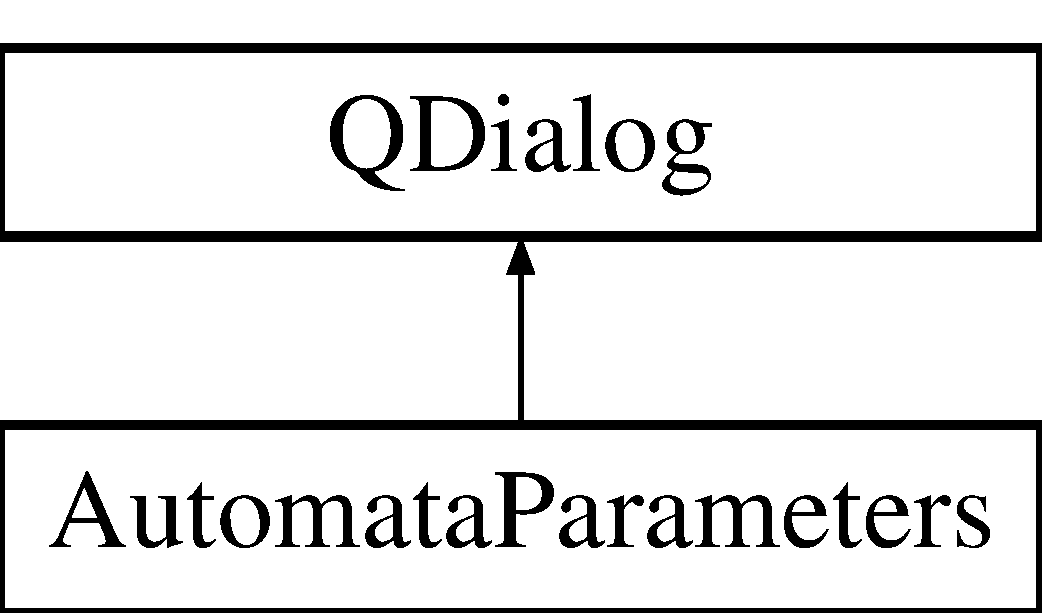
\includegraphics[height=2.000000cm]{class_automata_parameters}
\end{center}
\end{figure}
\subsection*{Public Member Functions}
\begin{DoxyCompactItemize}
\item 
\mbox{\hyperlink{class_automata_parameters_a67caea1bf676cb572a00da603732e7df}{Automata\+Parameters}} (Q\+Widget $\ast$parent=0, char def=\textquotesingle{}s\textquotesingle{}, \mbox{\hyperlink{automatamanager_8h_ae6fa959b9e8f9c638e0d82bf2c7dc5e7}{dim}} d=\mbox{\hyperlink{automatamanager_8h_ae6fa959b9e8f9c638e0d82bf2c7dc5e7a96ae589b7d5427dde9e5da18bbf68d86}{d2}})
\end{DoxyCompactItemize}
\subsection*{Private Attributes}
\begin{DoxyCompactItemize}
\item 
Q\+Tab\+Widget $\ast$ \mbox{\hyperlink{class_automata_parameters_aca77fcb495c7820c6d571684671e594b}{tab\+Widget}}
\item 
Q\+Line\+Edit $\ast$ \mbox{\hyperlink{class_automata_parameters_a03f985866b0f323e94b5a1d568fa052d}{column}}
\item 
Q\+Line\+Edit $\ast$ \mbox{\hyperlink{class_automata_parameters_a8823a82d6cb4f6ed9f1359e43500e30e}{row}}
\item 
Q\+Radio\+Button $\ast$ \mbox{\hyperlink{class_automata_parameters_ab81d709fa04c426c661c443c95284bd2}{dead}}
\item 
Q\+Radio\+Button $\ast$ \mbox{\hyperlink{class_automata_parameters_ac38a724b4bc923a1515b2fc0e075ccf6}{alive}}
\item 
Q\+Radio\+Button $\ast$ \mbox{\hyperlink{class_automata_parameters_a9f35c892bdbb5674713978eaac1864b3}{same}}
\item 
Q\+Spin\+Box $\ast$ \mbox{\hyperlink{class_automata_parameters_a5e7d624be5787381d22d85a48b3c1595}{neighbourhood}}
\item 
Q\+Check\+Box $\ast$ \mbox{\hyperlink{class_automata_parameters_a417b0bba086be74ed18a21ceb1e6d835}{random}}
\item 
Q\+Dialog\+Button\+Box $\ast$ \mbox{\hyperlink{class_automata_parameters_a4da6ee987dbbf3956a5167f75b72548a}{button\+Box}}
\end{DoxyCompactItemize}
\subsection*{Friends}
\begin{DoxyCompactItemize}
\item 
class \mbox{\hyperlink{class_automata_parameters_a154f5ffe46dc74c6c94311b4cc3927ae}{Main\+Controller}}
\end{DoxyCompactItemize}


\subsection{Constructor \& Destructor Documentation}
\mbox{\Hypertarget{class_automata_parameters_a67caea1bf676cb572a00da603732e7df}\label{class_automata_parameters_a67caea1bf676cb572a00da603732e7df}} 
\index{Automata\+Parameters@{Automata\+Parameters}!Automata\+Parameters@{Automata\+Parameters}}
\index{Automata\+Parameters@{Automata\+Parameters}!Automata\+Parameters@{Automata\+Parameters}}
\subsubsection{\texorpdfstring{Automata\+Parameters()}{AutomataParameters()}}
{\footnotesize\ttfamily Automata\+Parameters\+::\+Automata\+Parameters (\begin{DoxyParamCaption}\item[{Q\+Widget $\ast$}]{parent = {\ttfamily 0},  }\item[{char}]{def = {\ttfamily \textquotesingle{}s\textquotesingle{}},  }\item[{\mbox{\hyperlink{automatamanager_8h_ae6fa959b9e8f9c638e0d82bf2c7dc5e7}{dim}}}]{d = {\ttfamily \mbox{\hyperlink{automatamanager_8h_ae6fa959b9e8f9c638e0d82bf2c7dc5e7a96ae589b7d5427dde9e5da18bbf68d86}{d2}}} }\end{DoxyParamCaption})}



\subsection{Friends And Related Function Documentation}
\mbox{\Hypertarget{class_automata_parameters_a154f5ffe46dc74c6c94311b4cc3927ae}\label{class_automata_parameters_a154f5ffe46dc74c6c94311b4cc3927ae}} 
\index{Automata\+Parameters@{Automata\+Parameters}!Main\+Controller@{Main\+Controller}}
\index{Main\+Controller@{Main\+Controller}!Automata\+Parameters@{Automata\+Parameters}}
\subsubsection{\texorpdfstring{Main\+Controller}{MainController}}
{\footnotesize\ttfamily friend class \mbox{\hyperlink{class_main_controller}{Main\+Controller}}\hspace{0.3cm}{\ttfamily [friend]}}



\subsection{Member Data Documentation}
\mbox{\Hypertarget{class_automata_parameters_ac38a724b4bc923a1515b2fc0e075ccf6}\label{class_automata_parameters_ac38a724b4bc923a1515b2fc0e075ccf6}} 
\index{Automata\+Parameters@{Automata\+Parameters}!alive@{alive}}
\index{alive@{alive}!Automata\+Parameters@{Automata\+Parameters}}
\subsubsection{\texorpdfstring{alive}{alive}}
{\footnotesize\ttfamily Q\+Radio\+Button$\ast$ Automata\+Parameters\+::alive\hspace{0.3cm}{\ttfamily [private]}}

\mbox{\Hypertarget{class_automata_parameters_a4da6ee987dbbf3956a5167f75b72548a}\label{class_automata_parameters_a4da6ee987dbbf3956a5167f75b72548a}} 
\index{Automata\+Parameters@{Automata\+Parameters}!button\+Box@{button\+Box}}
\index{button\+Box@{button\+Box}!Automata\+Parameters@{Automata\+Parameters}}
\subsubsection{\texorpdfstring{button\+Box}{buttonBox}}
{\footnotesize\ttfamily Q\+Dialog\+Button\+Box$\ast$ Automata\+Parameters\+::button\+Box\hspace{0.3cm}{\ttfamily [private]}}

\mbox{\Hypertarget{class_automata_parameters_a03f985866b0f323e94b5a1d568fa052d}\label{class_automata_parameters_a03f985866b0f323e94b5a1d568fa052d}} 
\index{Automata\+Parameters@{Automata\+Parameters}!column@{column}}
\index{column@{column}!Automata\+Parameters@{Automata\+Parameters}}
\subsubsection{\texorpdfstring{column}{column}}
{\footnotesize\ttfamily Q\+Line\+Edit$\ast$ Automata\+Parameters\+::column\hspace{0.3cm}{\ttfamily [private]}}

\mbox{\Hypertarget{class_automata_parameters_ab81d709fa04c426c661c443c95284bd2}\label{class_automata_parameters_ab81d709fa04c426c661c443c95284bd2}} 
\index{Automata\+Parameters@{Automata\+Parameters}!dead@{dead}}
\index{dead@{dead}!Automata\+Parameters@{Automata\+Parameters}}
\subsubsection{\texorpdfstring{dead}{dead}}
{\footnotesize\ttfamily Q\+Radio\+Button$\ast$ Automata\+Parameters\+::dead\hspace{0.3cm}{\ttfamily [private]}}

\mbox{\Hypertarget{class_automata_parameters_a5e7d624be5787381d22d85a48b3c1595}\label{class_automata_parameters_a5e7d624be5787381d22d85a48b3c1595}} 
\index{Automata\+Parameters@{Automata\+Parameters}!neighbourhood@{neighbourhood}}
\index{neighbourhood@{neighbourhood}!Automata\+Parameters@{Automata\+Parameters}}
\subsubsection{\texorpdfstring{neighbourhood}{neighbourhood}}
{\footnotesize\ttfamily Q\+Spin\+Box$\ast$ Automata\+Parameters\+::neighbourhood\hspace{0.3cm}{\ttfamily [private]}}

\mbox{\Hypertarget{class_automata_parameters_a417b0bba086be74ed18a21ceb1e6d835}\label{class_automata_parameters_a417b0bba086be74ed18a21ceb1e6d835}} 
\index{Automata\+Parameters@{Automata\+Parameters}!random@{random}}
\index{random@{random}!Automata\+Parameters@{Automata\+Parameters}}
\subsubsection{\texorpdfstring{random}{random}}
{\footnotesize\ttfamily Q\+Check\+Box$\ast$ Automata\+Parameters\+::random\hspace{0.3cm}{\ttfamily [private]}}

\mbox{\Hypertarget{class_automata_parameters_a8823a82d6cb4f6ed9f1359e43500e30e}\label{class_automata_parameters_a8823a82d6cb4f6ed9f1359e43500e30e}} 
\index{Automata\+Parameters@{Automata\+Parameters}!row@{row}}
\index{row@{row}!Automata\+Parameters@{Automata\+Parameters}}
\subsubsection{\texorpdfstring{row}{row}}
{\footnotesize\ttfamily Q\+Line\+Edit$\ast$ Automata\+Parameters\+::row\hspace{0.3cm}{\ttfamily [private]}}

\mbox{\Hypertarget{class_automata_parameters_a9f35c892bdbb5674713978eaac1864b3}\label{class_automata_parameters_a9f35c892bdbb5674713978eaac1864b3}} 
\index{Automata\+Parameters@{Automata\+Parameters}!same@{same}}
\index{same@{same}!Automata\+Parameters@{Automata\+Parameters}}
\subsubsection{\texorpdfstring{same}{same}}
{\footnotesize\ttfamily Q\+Radio\+Button$\ast$ Automata\+Parameters\+::same\hspace{0.3cm}{\ttfamily [private]}}

\mbox{\Hypertarget{class_automata_parameters_aca77fcb495c7820c6d571684671e594b}\label{class_automata_parameters_aca77fcb495c7820c6d571684671e594b}} 
\index{Automata\+Parameters@{Automata\+Parameters}!tab\+Widget@{tab\+Widget}}
\index{tab\+Widget@{tab\+Widget}!Automata\+Parameters@{Automata\+Parameters}}
\subsubsection{\texorpdfstring{tab\+Widget}{tabWidget}}
{\footnotesize\ttfamily Q\+Tab\+Widget$\ast$ Automata\+Parameters\+::tab\+Widget\hspace{0.3cm}{\ttfamily [private]}}



The documentation for this class was generated from the following files\+:\begin{DoxyCompactItemize}
\item 
\mbox{\hyperlink{maincontroller_8h}{maincontroller.\+h}}\item 
\mbox{\hyperlink{maincontroller_8cpp}{maincontroller.\+cpp}}\end{DoxyCompactItemize}

\hypertarget{class_automaton}{}\section{Automaton Class Reference}
\label{class_automaton}\index{Automaton@{Automaton}}


{\ttfamily \#include $<$automaton.\+h$>$}

\subsection*{Classes}
\begin{DoxyCompactItemize}
\item 
struct \mbox{\hyperlink{struct_automaton_1_1_range}{Range}}
\begin{DoxyCompactList}\small\item\em Permet de stocker un intervalle. \end{DoxyCompactList}\end{DoxyCompactItemize}
\subsection*{Public Member Functions}
\begin{DoxyCompactItemize}
\item 
\mbox{\hyperlink{class_automaton_a6dee06d8b80717d8ac77e284871bb972}{Automaton}} (unsigned int nb, unsigned int \mbox{\hyperlink{automatamanager_8h_ae6fa959b9e8f9c638e0d82bf2c7dc5e7}{dim}}, char dn)
\begin{DoxyCompactList}\small\item\em Constructeur pour créer un nouvel automate. \end{DoxyCompactList}\item 
\mbox{\hyperlink{class_automaton_a30696da386c2b0119f41569272200e2c}{Automaton}} (const unsigned int id, sqlite3 $\ast$db)
\begin{DoxyCompactList}\small\item\em Constructeur à partir d\textquotesingle{}une base de donnees S\+QL. \end{DoxyCompactList}\item 
\mbox{\hyperlink{class_automaton_a1bd3904052977bba7901df924f1bef53}{Automaton}} (Q\+String const \&file\+Name)
\begin{DoxyCompactList}\small\item\em Constructeur à partir d\textquotesingle{}une Qstring. \end{DoxyCompactList}\item 
\mbox{\hyperlink{class_automaton_a6caf31920730c11d5fccc5918c8a3585}{Automaton}} (const std\+::string \&s)
\begin{DoxyCompactList}\small\item\em Constructeur à partir d\textquotesingle{}une std\+::string. \end{DoxyCompactList}\item 
char \mbox{\hyperlink{class_automaton_a6ce870e9a73694b40da41132198e7c31}{next}} (std\+::string s)
\begin{DoxyCompactList}\small\item\em Calcul l\textquotesingle{}état suivant à partir de la string des voisins. \end{DoxyCompactList}\item 
void \mbox{\hyperlink{class_automaton_ae77214bcd75f24d2cb56506e300a7991}{insert\+Position\+Rule}} (std\+::vector$<$ bool $>$ v, char c)
\begin{DoxyCompactList}\small\item\em Insere une règle de position dans l\textquotesingle{}arbre binaire. \end{DoxyCompactList}\item 
void \mbox{\hyperlink{class_automaton_ad5365dca1251e866c57412b65f666ba6}{insert\+Rule\+Nb\+Into}} (unsigned int a, unsigned int b, char c)
\begin{DoxyCompactList}\small\item\em Insere une règle sur le nombre de voisins de type donné \end{DoxyCompactList}\item 
void \mbox{\hyperlink{class_automaton_a622c489cd8cc82000c3256ca0c40f48d}{insert\+Range\+Into}} (std\+::vector$<$ \mbox{\hyperlink{struct_automaton_1_1_range}{Range}} $>$ \&coll, unsigned int a, unsigned int b)
\begin{DoxyCompactList}\small\item\em Insère un intervalle dans la collection specifiée. \end{DoxyCompactList}\item 
std\+::string \mbox{\hyperlink{class_automaton_a0870a8cd719c779a822780d455e33595}{serialize\+Nb\+Rules}} ()
\begin{DoxyCompactList}\small\item\em Serialise les règles de voisins en une std\+::string. \end{DoxyCompactList}\item 
void \mbox{\hyperlink{class_automaton_a86e17f607815376791dbb2490141007d}{deserialize\+Nb\+Rules}} (const std\+::string \&s)
\begin{DoxyCompactList}\small\item\em Deserialise les règles de voisins a partir d\textquotesingle{}une std\+::string. \end{DoxyCompactList}\item 
void \mbox{\hyperlink{class_automaton_ab2a707832bdd7daf40ddf7e99503c0f9}{deserialize}} (const std\+::string \&s)
\begin{DoxyCompactList}\small\item\em Deserialise à partir d\textquotesingle{}une std\+::string. \end{DoxyCompactList}\item 
unsigned int \mbox{\hyperlink{class_automaton_a1d4431d42cc2c71fef33c125d321b633}{save}} (const Q\+String \&name, sqlite3 $\ast$db)
\item 
void \mbox{\hyperlink{class_automaton_a054e743dde571a5fdf935ce431a468a7}{export\+To\+File}} (Q\+String const \&name)
\item 
unsigned int \mbox{\hyperlink{class_automaton_af61fbe8bf05c0b2223d7a67f3e429f3e}{getN}} ()
\item 
unsigned int \mbox{\hyperlink{class_automaton_a27b050dff4898c55c20e2950e54b2fc9}{get\+Dim}} ()
\end{DoxyCompactItemize}
\subsection*{Public Attributes}
\begin{DoxyCompactItemize}
\item 
unsigned int \mbox{\hyperlink{class_automaton_ac55590f74c2e26e198050887a62ec1cb}{n}}
\begin{DoxyCompactList}\small\item\em Nombre de voisins qui comptent pour l\textquotesingle{}état suivant. \end{DoxyCompactList}\item 
unsigned int \mbox{\hyperlink{class_automaton_a69ea9d67aba5ece34636fb95de1b487f}{dim}}
\begin{DoxyCompactList}\small\item\em Dimension\+: 1D ou 2D. \end{DoxyCompactList}\item 
char \mbox{\hyperlink{class_automaton_aa7894d8b17e4fe17553bca13e5b93cf5}{default\+Next}}
\begin{DoxyCompactList}\small\item\em Etat suivant par défaut. \end{DoxyCompactList}\item 
Rule\+Bst $\ast$ \mbox{\hyperlink{class_automaton_a3b344073044f20fcaba766e34ec24387}{rule\+Bst}}
\begin{DoxyCompactList}\small\item\em Arbre des positions d\textquotesingle{}états. \end{DoxyCompactList}\item 
std\+::vector$<$ \mbox{\hyperlink{struct_automaton_1_1_range}{Range}} $>$ \mbox{\hyperlink{class_automaton_afab3dec429a12d5c1e30c1691ec36c8c}{rule\+Nb\+Neighb\+Life}}
\begin{DoxyCompactList}\small\item\em Vecteur d\textquotesingle{}intervalles donnant la vie. \end{DoxyCompactList}\item 
std\+::vector$<$ \mbox{\hyperlink{struct_automaton_1_1_range}{Range}} $>$ \mbox{\hyperlink{class_automaton_a3c4b049f935fe17aa3fc7e40c7fa8f7f}{rule\+Nb\+Neighb\+Death}}
\begin{DoxyCompactList}\small\item\em Vecteur d\textquotesingle{}intervalles donnant la mort. \end{DoxyCompactList}\item 
std\+::vector$<$ \mbox{\hyperlink{struct_automaton_1_1_range}{Range}} $>$ \mbox{\hyperlink{class_automaton_a7a9a78c542bfdc9cb9c01ad268ae1485}{rule\+Nb\+Neighb\+Same}}
\begin{DoxyCompactList}\small\item\em Vecteur d\textquotesingle{}intervalles donnant un état identique. \end{DoxyCompactList}\end{DoxyCompactItemize}
\subsection*{Private Member Functions}
\begin{DoxyCompactItemize}
\item 
std\+::string \mbox{\hyperlink{class_automaton_a1f1af7879a469e3ad8c282d0a58a7da4}{serialize}} ()
\begin{DoxyCompactList}\small\item\em Serialise l\textquotesingle{}automate. \end{DoxyCompactList}\item 
\mbox{\hyperlink{class_automaton_a6400f21ac67170631963cbc29638ec8c}{Automaton}} ()=delete
\end{DoxyCompactItemize}


\subsection{Detailed Description}
Classe qui peut se résumer à un ensemble de règles. Possède également une méthode calculer l\textquotesingle{}état suivant 

\subsection{Constructor \& Destructor Documentation}
\mbox{\Hypertarget{class_automaton_a6400f21ac67170631963cbc29638ec8c}\label{class_automaton_a6400f21ac67170631963cbc29638ec8c}} 
\index{Automaton@{Automaton}!Automaton@{Automaton}}
\index{Automaton@{Automaton}!Automaton@{Automaton}}
\subsubsection{\texorpdfstring{Automaton()}{Automaton()}\hspace{0.1cm}{\footnotesize\ttfamily [1/5]}}
{\footnotesize\ttfamily Automaton\+::\+Automaton (\begin{DoxyParamCaption}{ }\end{DoxyParamCaption})\hspace{0.3cm}{\ttfamily [private]}, {\ttfamily [delete]}}

\mbox{\Hypertarget{class_automaton_a6dee06d8b80717d8ac77e284871bb972}\label{class_automaton_a6dee06d8b80717d8ac77e284871bb972}} 
\index{Automaton@{Automaton}!Automaton@{Automaton}}
\index{Automaton@{Automaton}!Automaton@{Automaton}}
\subsubsection{\texorpdfstring{Automaton()}{Automaton()}\hspace{0.1cm}{\footnotesize\ttfamily [2/5]}}
{\footnotesize\ttfamily Automaton\+::\+Automaton (\begin{DoxyParamCaption}\item[{unsigned int}]{nb,  }\item[{unsigned int}]{dim,  }\item[{char}]{dn }\end{DoxyParamCaption})\hspace{0.3cm}{\ttfamily [inline]}}



Constructeur pour créer un nouvel automate. 

\mbox{\Hypertarget{class_automaton_a30696da386c2b0119f41569272200e2c}\label{class_automaton_a30696da386c2b0119f41569272200e2c}} 
\index{Automaton@{Automaton}!Automaton@{Automaton}}
\index{Automaton@{Automaton}!Automaton@{Automaton}}
\subsubsection{\texorpdfstring{Automaton()}{Automaton()}\hspace{0.1cm}{\footnotesize\ttfamily [3/5]}}
{\footnotesize\ttfamily Automaton\+::\+Automaton (\begin{DoxyParamCaption}\item[{const unsigned int}]{id,  }\item[{sqlite3 $\ast$}]{db }\end{DoxyParamCaption})}



Constructeur à partir d\textquotesingle{}une base de donnees S\+QL. 

\mbox{\Hypertarget{class_automaton_a1bd3904052977bba7901df924f1bef53}\label{class_automaton_a1bd3904052977bba7901df924f1bef53}} 
\index{Automaton@{Automaton}!Automaton@{Automaton}}
\index{Automaton@{Automaton}!Automaton@{Automaton}}
\subsubsection{\texorpdfstring{Automaton()}{Automaton()}\hspace{0.1cm}{\footnotesize\ttfamily [4/5]}}
{\footnotesize\ttfamily Automaton\+::\+Automaton (\begin{DoxyParamCaption}\item[{Q\+String const \&}]{file\+Name }\end{DoxyParamCaption})}



Constructeur à partir d\textquotesingle{}une Qstring. 

\mbox{\Hypertarget{class_automaton_a6caf31920730c11d5fccc5918c8a3585}\label{class_automaton_a6caf31920730c11d5fccc5918c8a3585}} 
\index{Automaton@{Automaton}!Automaton@{Automaton}}
\index{Automaton@{Automaton}!Automaton@{Automaton}}
\subsubsection{\texorpdfstring{Automaton()}{Automaton()}\hspace{0.1cm}{\footnotesize\ttfamily [5/5]}}
{\footnotesize\ttfamily Automaton\+::\+Automaton (\begin{DoxyParamCaption}\item[{const std\+::string \&}]{s }\end{DoxyParamCaption})\hspace{0.3cm}{\ttfamily [inline]}}



Constructeur à partir d\textquotesingle{}une std\+::string. 



\subsection{Member Function Documentation}
\mbox{\Hypertarget{class_automaton_ab2a707832bdd7daf40ddf7e99503c0f9}\label{class_automaton_ab2a707832bdd7daf40ddf7e99503c0f9}} 
\index{Automaton@{Automaton}!deserialize@{deserialize}}
\index{deserialize@{deserialize}!Automaton@{Automaton}}
\subsubsection{\texorpdfstring{deserialize()}{deserialize()}}
{\footnotesize\ttfamily void Automaton\+::deserialize (\begin{DoxyParamCaption}\item[{const std\+::string \&}]{s }\end{DoxyParamCaption})}



Deserialise à partir d\textquotesingle{}une std\+::string. 

\mbox{\Hypertarget{class_automaton_a86e17f607815376791dbb2490141007d}\label{class_automaton_a86e17f607815376791dbb2490141007d}} 
\index{Automaton@{Automaton}!deserialize\+Nb\+Rules@{deserialize\+Nb\+Rules}}
\index{deserialize\+Nb\+Rules@{deserialize\+Nb\+Rules}!Automaton@{Automaton}}
\subsubsection{\texorpdfstring{deserialize\+Nb\+Rules()}{deserializeNbRules()}}
{\footnotesize\ttfamily void Automaton\+::deserialize\+Nb\+Rules (\begin{DoxyParamCaption}\item[{const std\+::string \&}]{s }\end{DoxyParamCaption})}



Deserialise les règles de voisins a partir d\textquotesingle{}une std\+::string. 

\mbox{\Hypertarget{class_automaton_a054e743dde571a5fdf935ce431a468a7}\label{class_automaton_a054e743dde571a5fdf935ce431a468a7}} 
\index{Automaton@{Automaton}!export\+To\+File@{export\+To\+File}}
\index{export\+To\+File@{export\+To\+File}!Automaton@{Automaton}}
\subsubsection{\texorpdfstring{export\+To\+File()}{exportToFile()}}
{\footnotesize\ttfamily void Automaton\+::export\+To\+File (\begin{DoxyParamCaption}\item[{Q\+String const \&}]{name }\end{DoxyParamCaption})}

\mbox{\Hypertarget{class_automaton_a27b050dff4898c55c20e2950e54b2fc9}\label{class_automaton_a27b050dff4898c55c20e2950e54b2fc9}} 
\index{Automaton@{Automaton}!get\+Dim@{get\+Dim}}
\index{get\+Dim@{get\+Dim}!Automaton@{Automaton}}
\subsubsection{\texorpdfstring{get\+Dim()}{getDim()}}
{\footnotesize\ttfamily unsigned int Automaton\+::get\+Dim (\begin{DoxyParamCaption}{ }\end{DoxyParamCaption})\hspace{0.3cm}{\ttfamily [inline]}}

\mbox{\Hypertarget{class_automaton_af61fbe8bf05c0b2223d7a67f3e429f3e}\label{class_automaton_af61fbe8bf05c0b2223d7a67f3e429f3e}} 
\index{Automaton@{Automaton}!getN@{getN}}
\index{getN@{getN}!Automaton@{Automaton}}
\subsubsection{\texorpdfstring{get\+N()}{getN()}}
{\footnotesize\ttfamily unsigned int Automaton\+::getN (\begin{DoxyParamCaption}{ }\end{DoxyParamCaption})\hspace{0.3cm}{\ttfamily [inline]}}

\mbox{\Hypertarget{class_automaton_ae77214bcd75f24d2cb56506e300a7991}\label{class_automaton_ae77214bcd75f24d2cb56506e300a7991}} 
\index{Automaton@{Automaton}!insert\+Position\+Rule@{insert\+Position\+Rule}}
\index{insert\+Position\+Rule@{insert\+Position\+Rule}!Automaton@{Automaton}}
\subsubsection{\texorpdfstring{insert\+Position\+Rule()}{insertPositionRule()}}
{\footnotesize\ttfamily void Automaton\+::insert\+Position\+Rule (\begin{DoxyParamCaption}\item[{std\+::vector$<$ bool $>$}]{v,  }\item[{char}]{c }\end{DoxyParamCaption})\hspace{0.3cm}{\ttfamily [inline]}}



Insere une règle de position dans l\textquotesingle{}arbre binaire. 

\mbox{\Hypertarget{class_automaton_a622c489cd8cc82000c3256ca0c40f48d}\label{class_automaton_a622c489cd8cc82000c3256ca0c40f48d}} 
\index{Automaton@{Automaton}!insert\+Range\+Into@{insert\+Range\+Into}}
\index{insert\+Range\+Into@{insert\+Range\+Into}!Automaton@{Automaton}}
\subsubsection{\texorpdfstring{insert\+Range\+Into()}{insertRangeInto()}}
{\footnotesize\ttfamily void Automaton\+::insert\+Range\+Into (\begin{DoxyParamCaption}\item[{std\+::vector$<$ \mbox{\hyperlink{struct_automaton_1_1_range}{Range}} $>$ \&}]{coll,  }\item[{unsigned int}]{a,  }\item[{unsigned int}]{b }\end{DoxyParamCaption})}



Insère un intervalle dans la collection specifiée. 

\mbox{\Hypertarget{class_automaton_ad5365dca1251e866c57412b65f666ba6}\label{class_automaton_ad5365dca1251e866c57412b65f666ba6}} 
\index{Automaton@{Automaton}!insert\+Rule\+Nb\+Into@{insert\+Rule\+Nb\+Into}}
\index{insert\+Rule\+Nb\+Into@{insert\+Rule\+Nb\+Into}!Automaton@{Automaton}}
\subsubsection{\texorpdfstring{insert\+Rule\+Nb\+Into()}{insertRuleNbInto()}}
{\footnotesize\ttfamily void Automaton\+::insert\+Rule\+Nb\+Into (\begin{DoxyParamCaption}\item[{unsigned int}]{a,  }\item[{unsigned int}]{b,  }\item[{char}]{c }\end{DoxyParamCaption})\hspace{0.3cm}{\ttfamily [inline]}}



Insere une règle sur le nombre de voisins de type donné 

\mbox{\Hypertarget{class_automaton_a6ce870e9a73694b40da41132198e7c31}\label{class_automaton_a6ce870e9a73694b40da41132198e7c31}} 
\index{Automaton@{Automaton}!next@{next}}
\index{next@{next}!Automaton@{Automaton}}
\subsubsection{\texorpdfstring{next()}{next()}}
{\footnotesize\ttfamily char Automaton\+::next (\begin{DoxyParamCaption}\item[{std\+::string}]{s }\end{DoxyParamCaption})}



Calcul l\textquotesingle{}état suivant à partir de la string des voisins. 

\mbox{\Hypertarget{class_automaton_a1d4431d42cc2c71fef33c125d321b633}\label{class_automaton_a1d4431d42cc2c71fef33c125d321b633}} 
\index{Automaton@{Automaton}!save@{save}}
\index{save@{save}!Automaton@{Automaton}}
\subsubsection{\texorpdfstring{save()}{save()}}
{\footnotesize\ttfamily unsigned int Automaton\+::save (\begin{DoxyParamCaption}\item[{const Q\+String \&}]{name,  }\item[{sqlite3 $\ast$}]{db }\end{DoxyParamCaption})}

\mbox{\Hypertarget{class_automaton_a1f1af7879a469e3ad8c282d0a58a7da4}\label{class_automaton_a1f1af7879a469e3ad8c282d0a58a7da4}} 
\index{Automaton@{Automaton}!serialize@{serialize}}
\index{serialize@{serialize}!Automaton@{Automaton}}
\subsubsection{\texorpdfstring{serialize()}{serialize()}}
{\footnotesize\ttfamily std\+::string Automaton\+::serialize (\begin{DoxyParamCaption}{ }\end{DoxyParamCaption})\hspace{0.3cm}{\ttfamily [private]}}



Serialise l\textquotesingle{}automate. 

\mbox{\Hypertarget{class_automaton_a0870a8cd719c779a822780d455e33595}\label{class_automaton_a0870a8cd719c779a822780d455e33595}} 
\index{Automaton@{Automaton}!serialize\+Nb\+Rules@{serialize\+Nb\+Rules}}
\index{serialize\+Nb\+Rules@{serialize\+Nb\+Rules}!Automaton@{Automaton}}
\subsubsection{\texorpdfstring{serialize\+Nb\+Rules()}{serializeNbRules()}}
{\footnotesize\ttfamily std\+::string Automaton\+::serialize\+Nb\+Rules (\begin{DoxyParamCaption}{ }\end{DoxyParamCaption})}



Serialise les règles de voisins en une std\+::string. 



\subsection{Member Data Documentation}
\mbox{\Hypertarget{class_automaton_aa7894d8b17e4fe17553bca13e5b93cf5}\label{class_automaton_aa7894d8b17e4fe17553bca13e5b93cf5}} 
\index{Automaton@{Automaton}!default\+Next@{default\+Next}}
\index{default\+Next@{default\+Next}!Automaton@{Automaton}}
\subsubsection{\texorpdfstring{default\+Next}{defaultNext}}
{\footnotesize\ttfamily char Automaton\+::default\+Next}



Etat suivant par défaut. 

\mbox{\Hypertarget{class_automaton_a69ea9d67aba5ece34636fb95de1b487f}\label{class_automaton_a69ea9d67aba5ece34636fb95de1b487f}} 
\index{Automaton@{Automaton}!dim@{dim}}
\index{dim@{dim}!Automaton@{Automaton}}
\subsubsection{\texorpdfstring{dim}{dim}}
{\footnotesize\ttfamily unsigned int Automaton\+::dim}



Dimension\+: 1D ou 2D. 

\mbox{\Hypertarget{class_automaton_ac55590f74c2e26e198050887a62ec1cb}\label{class_automaton_ac55590f74c2e26e198050887a62ec1cb}} 
\index{Automaton@{Automaton}!n@{n}}
\index{n@{n}!Automaton@{Automaton}}
\subsubsection{\texorpdfstring{n}{n}}
{\footnotesize\ttfamily unsigned int Automaton\+::n}



Nombre de voisins qui comptent pour l\textquotesingle{}état suivant. 

\mbox{\Hypertarget{class_automaton_a3b344073044f20fcaba766e34ec24387}\label{class_automaton_a3b344073044f20fcaba766e34ec24387}} 
\index{Automaton@{Automaton}!rule\+Bst@{rule\+Bst}}
\index{rule\+Bst@{rule\+Bst}!Automaton@{Automaton}}
\subsubsection{\texorpdfstring{rule\+Bst}{ruleBst}}
{\footnotesize\ttfamily Rule\+Bst$\ast$ Automaton\+::rule\+Bst}



Arbre des positions d\textquotesingle{}états. 

\mbox{\Hypertarget{class_automaton_a3c4b049f935fe17aa3fc7e40c7fa8f7f}\label{class_automaton_a3c4b049f935fe17aa3fc7e40c7fa8f7f}} 
\index{Automaton@{Automaton}!rule\+Nb\+Neighb\+Death@{rule\+Nb\+Neighb\+Death}}
\index{rule\+Nb\+Neighb\+Death@{rule\+Nb\+Neighb\+Death}!Automaton@{Automaton}}
\subsubsection{\texorpdfstring{rule\+Nb\+Neighb\+Death}{ruleNbNeighbDeath}}
{\footnotesize\ttfamily std\+::vector$<$\mbox{\hyperlink{struct_automaton_1_1_range}{Range}}$>$ Automaton\+::rule\+Nb\+Neighb\+Death}



Vecteur d\textquotesingle{}intervalles donnant la mort. 

\mbox{\Hypertarget{class_automaton_afab3dec429a12d5c1e30c1691ec36c8c}\label{class_automaton_afab3dec429a12d5c1e30c1691ec36c8c}} 
\index{Automaton@{Automaton}!rule\+Nb\+Neighb\+Life@{rule\+Nb\+Neighb\+Life}}
\index{rule\+Nb\+Neighb\+Life@{rule\+Nb\+Neighb\+Life}!Automaton@{Automaton}}
\subsubsection{\texorpdfstring{rule\+Nb\+Neighb\+Life}{ruleNbNeighbLife}}
{\footnotesize\ttfamily std\+::vector$<$\mbox{\hyperlink{struct_automaton_1_1_range}{Range}}$>$ Automaton\+::rule\+Nb\+Neighb\+Life}



Vecteur d\textquotesingle{}intervalles donnant la vie. 

\mbox{\Hypertarget{class_automaton_a7a9a78c542bfdc9cb9c01ad268ae1485}\label{class_automaton_a7a9a78c542bfdc9cb9c01ad268ae1485}} 
\index{Automaton@{Automaton}!rule\+Nb\+Neighb\+Same@{rule\+Nb\+Neighb\+Same}}
\index{rule\+Nb\+Neighb\+Same@{rule\+Nb\+Neighb\+Same}!Automaton@{Automaton}}
\subsubsection{\texorpdfstring{rule\+Nb\+Neighb\+Same}{ruleNbNeighbSame}}
{\footnotesize\ttfamily std\+::vector$<$\mbox{\hyperlink{struct_automaton_1_1_range}{Range}}$>$ Automaton\+::rule\+Nb\+Neighb\+Same}



Vecteur d\textquotesingle{}intervalles donnant un état identique. 



The documentation for this class was generated from the following files\+:\begin{DoxyCompactItemize}
\item 
\mbox{\hyperlink{automaton_8h}{automaton.\+h}}\item 
\mbox{\hyperlink{automaton_8cpp}{automaton.\+cpp}}\end{DoxyCompactItemize}

\hypertarget{class_automata_manager_1_1_automaton_description}{}\section{Automata\+Manager\+:\+:Automaton\+Description Class Reference}
\label{class_automata_manager_1_1_automaton_description}\index{Automata\+Manager\+::\+Automaton\+Description@{Automata\+Manager\+::\+Automaton\+Description}}


Classe interne permettant de stocker les informations des automates venus de la B\+DD.  




{\ttfamily \#include $<$automatamanager.\+h$>$}

\subsection*{Public Member Functions}
\begin{DoxyCompactItemize}
\item 
\mbox{\hyperlink{class_automata_manager_1_1_automaton_description_a48061cac5f3504b783a9949dfab6fefa}{Automaton\+Description}} (unsigned int i, Q\+String n, \mbox{\hyperlink{automatamanager_8h_ae6fa959b9e8f9c638e0d82bf2c7dc5e7}{dim}} d)
\begin{DoxyCompactList}\small\item\em La dimension de l\textquotesingle{}automate. \end{DoxyCompactList}\item 
unsigned int \mbox{\hyperlink{class_automata_manager_1_1_automaton_description_af88c7761e97cce2c29f25cc2785aad32}{get\+Id}} () const
\item 
const Q\+String \& \mbox{\hyperlink{class_automata_manager_1_1_automaton_description_aa84f4a3b752e9d12a84fe622c1a580c6}{get\+Name}} () const
\item 
\mbox{\hyperlink{automatamanager_8h_ae6fa959b9e8f9c638e0d82bf2c7dc5e7}{dim}} \mbox{\hyperlink{class_automata_manager_1_1_automaton_description_ac63a29de02d4862fb41b3beba034b839}{get\+Dimension}} () const
\end{DoxyCompactItemize}
\subsection*{Private Attributes}
\begin{DoxyCompactItemize}
\item 
unsigned int \mbox{\hyperlink{class_automata_manager_1_1_automaton_description_a49ea94482dc533e49506a4b50f23c404}{id}}
\item 
Q\+String \mbox{\hyperlink{class_automata_manager_1_1_automaton_description_a5a10b5598482bcf7e3c8f871a3e16dad}{name}}
\begin{DoxyCompactList}\small\item\em L\textquotesingle{}id de l\textquotesingle{}automate dans la B\+DD. \end{DoxyCompactList}\item 
\mbox{\hyperlink{automatamanager_8h_ae6fa959b9e8f9c638e0d82bf2c7dc5e7}{dim}} \mbox{\hyperlink{class_automata_manager_1_1_automaton_description_a1791ce5195bafc49fe4d4df74b25c82d}{dimension}}
\begin{DoxyCompactList}\small\item\em Le nom de l\textquotesingle{}automate. \end{DoxyCompactList}\end{DoxyCompactItemize}


\subsection{Detailed Description}
Classe interne permettant de stocker les informations des automates venus de la B\+DD. 

\subsection{Constructor \& Destructor Documentation}
\mbox{\Hypertarget{class_automata_manager_1_1_automaton_description_a48061cac5f3504b783a9949dfab6fefa}\label{class_automata_manager_1_1_automaton_description_a48061cac5f3504b783a9949dfab6fefa}} 
\index{Automata\+Manager\+::\+Automaton\+Description@{Automata\+Manager\+::\+Automaton\+Description}!Automaton\+Description@{Automaton\+Description}}
\index{Automaton\+Description@{Automaton\+Description}!Automata\+Manager\+::\+Automaton\+Description@{Automata\+Manager\+::\+Automaton\+Description}}
\subsubsection{\texorpdfstring{Automaton\+Description()}{AutomatonDescription()}}
{\footnotesize\ttfamily Automata\+Manager\+::\+Automaton\+Description\+::\+Automaton\+Description (\begin{DoxyParamCaption}\item[{unsigned int}]{i,  }\item[{Q\+String}]{n,  }\item[{\mbox{\hyperlink{automatamanager_8h_ae6fa959b9e8f9c638e0d82bf2c7dc5e7}{dim}}}]{d }\end{DoxyParamCaption})}



La dimension de l\textquotesingle{}automate. 



\subsection{Member Function Documentation}
\mbox{\Hypertarget{class_automata_manager_1_1_automaton_description_ac63a29de02d4862fb41b3beba034b839}\label{class_automata_manager_1_1_automaton_description_ac63a29de02d4862fb41b3beba034b839}} 
\index{Automata\+Manager\+::\+Automaton\+Description@{Automata\+Manager\+::\+Automaton\+Description}!get\+Dimension@{get\+Dimension}}
\index{get\+Dimension@{get\+Dimension}!Automata\+Manager\+::\+Automaton\+Description@{Automata\+Manager\+::\+Automaton\+Description}}
\subsubsection{\texorpdfstring{get\+Dimension()}{getDimension()}}
{\footnotesize\ttfamily \mbox{\hyperlink{automatamanager_8h_ae6fa959b9e8f9c638e0d82bf2c7dc5e7}{dim}} Automata\+Manager\+::\+Automaton\+Description\+::get\+Dimension (\begin{DoxyParamCaption}{ }\end{DoxyParamCaption}) const}

\mbox{\Hypertarget{class_automata_manager_1_1_automaton_description_af88c7761e97cce2c29f25cc2785aad32}\label{class_automata_manager_1_1_automaton_description_af88c7761e97cce2c29f25cc2785aad32}} 
\index{Automata\+Manager\+::\+Automaton\+Description@{Automata\+Manager\+::\+Automaton\+Description}!get\+Id@{get\+Id}}
\index{get\+Id@{get\+Id}!Automata\+Manager\+::\+Automaton\+Description@{Automata\+Manager\+::\+Automaton\+Description}}
\subsubsection{\texorpdfstring{get\+Id()}{getId()}}
{\footnotesize\ttfamily unsigned int Automata\+Manager\+::\+Automaton\+Description\+::get\+Id (\begin{DoxyParamCaption}{ }\end{DoxyParamCaption}) const}

\mbox{\Hypertarget{class_automata_manager_1_1_automaton_description_aa84f4a3b752e9d12a84fe622c1a580c6}\label{class_automata_manager_1_1_automaton_description_aa84f4a3b752e9d12a84fe622c1a580c6}} 
\index{Automata\+Manager\+::\+Automaton\+Description@{Automata\+Manager\+::\+Automaton\+Description}!get\+Name@{get\+Name}}
\index{get\+Name@{get\+Name}!Automata\+Manager\+::\+Automaton\+Description@{Automata\+Manager\+::\+Automaton\+Description}}
\subsubsection{\texorpdfstring{get\+Name()}{getName()}}
{\footnotesize\ttfamily const Q\+String \& Automata\+Manager\+::\+Automaton\+Description\+::get\+Name (\begin{DoxyParamCaption}{ }\end{DoxyParamCaption}) const}



\subsection{Member Data Documentation}
\mbox{\Hypertarget{class_automata_manager_1_1_automaton_description_a1791ce5195bafc49fe4d4df74b25c82d}\label{class_automata_manager_1_1_automaton_description_a1791ce5195bafc49fe4d4df74b25c82d}} 
\index{Automata\+Manager\+::\+Automaton\+Description@{Automata\+Manager\+::\+Automaton\+Description}!dimension@{dimension}}
\index{dimension@{dimension}!Automata\+Manager\+::\+Automaton\+Description@{Automata\+Manager\+::\+Automaton\+Description}}
\subsubsection{\texorpdfstring{dimension}{dimension}}
{\footnotesize\ttfamily \mbox{\hyperlink{automatamanager_8h_ae6fa959b9e8f9c638e0d82bf2c7dc5e7}{dim}} Automata\+Manager\+::\+Automaton\+Description\+::dimension\hspace{0.3cm}{\ttfamily [private]}}



Le nom de l\textquotesingle{}automate. 

\mbox{\Hypertarget{class_automata_manager_1_1_automaton_description_a49ea94482dc533e49506a4b50f23c404}\label{class_automata_manager_1_1_automaton_description_a49ea94482dc533e49506a4b50f23c404}} 
\index{Automata\+Manager\+::\+Automaton\+Description@{Automata\+Manager\+::\+Automaton\+Description}!id@{id}}
\index{id@{id}!Automata\+Manager\+::\+Automaton\+Description@{Automata\+Manager\+::\+Automaton\+Description}}
\subsubsection{\texorpdfstring{id}{id}}
{\footnotesize\ttfamily unsigned int Automata\+Manager\+::\+Automaton\+Description\+::id\hspace{0.3cm}{\ttfamily [private]}}

\mbox{\Hypertarget{class_automata_manager_1_1_automaton_description_a5a10b5598482bcf7e3c8f871a3e16dad}\label{class_automata_manager_1_1_automaton_description_a5a10b5598482bcf7e3c8f871a3e16dad}} 
\index{Automata\+Manager\+::\+Automaton\+Description@{Automata\+Manager\+::\+Automaton\+Description}!name@{name}}
\index{name@{name}!Automata\+Manager\+::\+Automaton\+Description@{Automata\+Manager\+::\+Automaton\+Description}}
\subsubsection{\texorpdfstring{name}{name}}
{\footnotesize\ttfamily Q\+String Automata\+Manager\+::\+Automaton\+Description\+::name\hspace{0.3cm}{\ttfamily [private]}}



L\textquotesingle{}id de l\textquotesingle{}automate dans la B\+DD. 



The documentation for this class was generated from the following files\+:\begin{DoxyCompactItemize}
\item 
\mbox{\hyperlink{automatamanager_8h}{automatamanager.\+h}}\item 
\mbox{\hyperlink{automatamanager_8cpp}{automatamanager.\+cpp}}\end{DoxyCompactItemize}

\hypertarget{class_main_controller}{}\section{Main\+Controller Class Reference}
\label{class_main_controller}\index{Main\+Controller@{Main\+Controller}}


{\ttfamily \#include $<$maincontroller.\+h$>$}

Inheritance diagram for Main\+Controller\+:\begin{figure}[H]
\begin{center}
\leavevmode
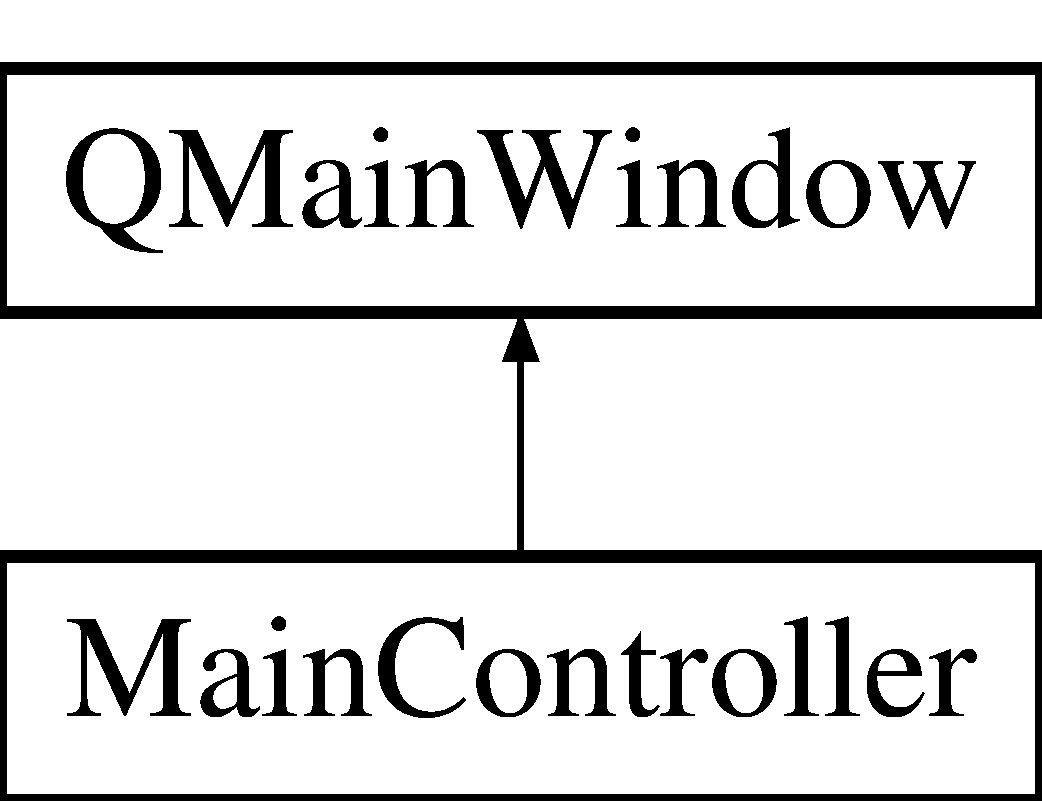
\includegraphics[height=2.000000cm]{class_main_controller}
\end{center}
\end{figure}
\subsection*{Public Member Functions}
\begin{DoxyCompactItemize}
\item 
\mbox{\hyperlink{class_main_controller_afc816e394f59614efba13d0657a0a351}{Main\+Controller}} ()
\begin{DoxyCompactList}\small\item\em Constructeur de la classe \mbox{\hyperlink{class_main_controller}{Main\+Controller}}. \end{DoxyCompactList}\end{DoxyCompactItemize}
\subsection*{Private Member Functions}
\begin{DoxyCompactItemize}
\item 
void \mbox{\hyperlink{class_main_controller_a26b5150d08fd0fecf209c3c8cd5c60b0}{create\+Actions}} ()
\begin{DoxyCompactList}\small\item\em create\+Actions \end{DoxyCompactList}\item 
void \mbox{\hyperlink{class_main_controller_a4d0f5b5351dcda6ce6e46fc606f916fb}{create\+Menus}} ()
\begin{DoxyCompactList}\small\item\em Initialisation des menus File et Edit. \end{DoxyCompactList}\item 
void \mbox{\hyperlink{class_main_controller_a141a116374c3605e54325bba6eaddb94}{create\+Tool\+Bars}} ()
\begin{DoxyCompactList}\small\item\em Initialisation des toolbars file\+Tool\+Bar et edit\+Tool\+Bar. \end{DoxyCompactList}\item 
Q\+String \mbox{\hyperlink{class_main_controller_a8cdfea32087af71164493b68c493a0e5}{open\+File}} ()
\item 
void \mbox{\hyperlink{class_main_controller_a48891e5a376e8315956222690238938f}{insert\+New\+Action}} (Q\+Menu $\ast$menu, int id, const Q\+String \&name, void(Automata\+Manager\+::$\ast$)(unsigned int const))
\begin{DoxyCompactList}\small\item\em Fonction générique permettant d\textquotesingle{}ajouter des Q\+Actions à un sous-\/menu, en mettant en tête de liste le dernier item selectionné \end{DoxyCompactList}\item 
void \mbox{\hyperlink{class_main_controller_ad0d31c3c005bf1ba9fda39455965ca0a}{new\+Automaton}} ()
\begin{DoxyCompactList}\small\item\em Instanction de la classe \mbox{\hyperlink{class_automata_parameters}{Automata\+Parameters}} depuis le \mbox{\hyperlink{class_main_controller}{Main\+Controller}}. On vérifie s\textquotesingle{}il existe déjà un automate créé. Si oui, on demande validation à l\textquotesingle{}utilisateur avant d\textquotesingle{}écraser l\textquotesingle{}automate courant. Sinon, on crée un nouvel automate. \end{DoxyCompactList}\item 
void \mbox{\hyperlink{class_main_controller_ae5a21e0d0566b2963618e822ad9d5f74}{new\+Automaton\+Next}} ()
\begin{DoxyCompactList}\small\item\em Permet de transmettre les différents paramètres entrés par l\textquotesingle{}utilisateur dans \mbox{\hyperlink{class_automata_parameters}{Automata\+Parameters}}, et de définir l\textquotesingle{}état initial du modèle relié à la vue. La fenêtre principale de l\textquotesingle{}application est actualisée en conséquence selon si 1D, 2D et/ou random. \end{DoxyCompactList}\item 
void \mbox{\hyperlink{class_main_controller_a8083c60cac9d1982633ad543900280a7}{new\+Rule}} ()
\begin{DoxyCompactList}\small\item\em Instanciation de la classe \mbox{\hyperlink{class_rules_controller}{Rules\+Controller}} par le \mbox{\hyperlink{class_main_controller}{Main\+Controller}}. On vérifie qu\textquotesingle{}il existe bien un automate avant d\textquotesingle{}ajouter une règle, et on transmet la dimension de l\textquotesingle{}automate au constructeur de règles. \end{DoxyCompactList}\end{DoxyCompactItemize}
\subsection*{Private Attributes}
\begin{DoxyCompactItemize}
\item 
\mbox{\hyperlink{class_automata_manager}{Automata\+Manager}} \& \mbox{\hyperlink{class_main_controller_ad926f088465fb1b7bbb181a4502aaad0}{instance}}
\item 
\mbox{\hyperlink{class_matrix_controller}{Matrix\+Controller}} $\ast$ \mbox{\hyperlink{class_main_controller_a24cdae20cbd62e663687fa079c23e83a}{view}}
\item 
\mbox{\hyperlink{class_automata_parameters}{Automata\+Parameters}} $\ast$ \mbox{\hyperlink{class_main_controller_a2c25d49c63992a3b1bcf312c2e02bb23}{param}}
\item 
Q\+Menu $\ast$ \mbox{\hyperlink{class_main_controller_a9b3df60ee05928b0296baf0b1051f261}{file\+Menu}}
\item 
Q\+Menu $\ast$ \mbox{\hyperlink{class_main_controller_a5ab07a811583fbca2549dbcd9919f71c}{edit\+Menu}}
\item 
Q\+Menu $\ast$ \mbox{\hyperlink{class_main_controller_a5242aa3227785bd402ab0e0e45d076e4}{sub\+Menu\+Automata}}
\item 
Q\+Menu $\ast$ \mbox{\hyperlink{class_main_controller_abbba1dcac884825de03d3b98835a7234}{sub\+Menu\+Grid}}
\item 
Q\+Tool\+Bar $\ast$ \mbox{\hyperlink{class_main_controller_a7c3800aaf55172aa565065272418f7f4}{file\+Tool\+Bar}}
\item 
Q\+Tool\+Bar $\ast$ \mbox{\hyperlink{class_main_controller_aee0527d0771c64102a9a3cdeb59024b0}{edit\+Tool\+Bar}}
\item 
Q\+Push\+Button $\ast$ \mbox{\hyperlink{class_main_controller_a710fae19858502fb93e097f12dca31f1}{play}}
\item 
Q\+Push\+Button $\ast$ \mbox{\hyperlink{class_main_controller_a76a6260f498cf6375d49e041a15ed2a3}{pause}}
\item 
Q\+Push\+Button $\ast$ \mbox{\hyperlink{class_main_controller_a122c813df75cca4a64b986ce826bb5a9}{random\+Button}}
\item 
Q\+Check\+Box $\ast$ \mbox{\hyperlink{class_main_controller_ac2739da22542b801ef4859087208cf54}{animation}}
\item 
Q\+Dial $\ast$ \mbox{\hyperlink{class_main_controller_a6c3d268678f6be5a53f30cc3c4a9aae3}{timer}}
\item 
Q\+L\+C\+D\+Number $\ast$ \mbox{\hyperlink{class_main_controller_a663d9bd8f3ca551a0634c9ff6e65be77}{lcd}}
\item 
Q\+Action $\ast$ \mbox{\hyperlink{class_main_controller_aa4e27060ff692d2e336d89534d437ec5}{New\+Automaton}}
\item 
Q\+Action $\ast$ \mbox{\hyperlink{class_main_controller_aa0379ddfda571ec99218a2fb0a1b205c}{Import\+Automaton}}
\item 
Q\+Action $\ast$ \mbox{\hyperlink{class_main_controller_a5457e18d4c2df72f7c5684d7ead37346}{Import\+Grid}}
\item 
Q\+Action $\ast$ \mbox{\hyperlink{class_main_controller_acf34814052183a7b16b799073b0f7d42}{Open\+Recent\+Automata}}
\item 
Q\+Action $\ast$ \mbox{\hyperlink{class_main_controller_a88ac3d205cf726f1d354a1944cfccfa0}{Open\+Recent\+Grid}}
\item 
Q\+Action $\ast$ \mbox{\hyperlink{class_main_controller_aea174540239231764b8abdfc7d62b900}{Save\+Automaton}}
\item 
Q\+Action $\ast$ \mbox{\hyperlink{class_main_controller_a4a10844a4ef8fa3ea5918f881d39da17}{Save\+Automaton\+As}}
\item 
Q\+Action $\ast$ \mbox{\hyperlink{class_main_controller_ad0e894d761ecd9367868ea39694a9e33}{Save\+Initial\+Grid}}
\item 
Q\+Action $\ast$ \mbox{\hyperlink{class_main_controller_abe302a428893230967ead1c5612a2c10}{Save\+Current\+Grid}}
\item 
Q\+Action $\ast$ \mbox{\hyperlink{class_main_controller_abfbbaa5a2ca58e3c3eb23c7ec2512273}{Export\+Automaton}}
\item 
Q\+Action $\ast$ \mbox{\hyperlink{class_main_controller_ac4da878595e3190049a7fee30f360537}{Export\+Current\+Grid}}
\item 
Q\+Action $\ast$ \mbox{\hyperlink{class_main_controller_ae348be948bfabf7f1756792d85d2c3a7}{Export\+Initial\+Grid}}
\item 
Q\+Action $\ast$ \mbox{\hyperlink{class_main_controller_a5db737ac032ba58ba169a7ecf95c1a56}{Exit}}
\item 
Q\+Action $\ast$ \mbox{\hyperlink{class_main_controller_af37c04bcfa78a77f2e7d717a5afa89e1}{New\+Rule}}
\item 
Q\+Action $\ast$ \mbox{\hyperlink{class_main_controller_a6bf8a7e4bd6677520dd6dcbd6659f5f3}{Set\+Timer}}
\item 
Q\+Action $\ast$ \mbox{\hyperlink{class_main_controller_a1ac3369371a9809fb9a20bbe138c220c}{Next\+Step}}
\item 
Q\+Widget $\ast$ \mbox{\hyperlink{class_main_controller_a2a3c3891d166eb53dff1422783687c18}{main\+Controller}}
\item 
Q\+H\+Box\+Layout $\ast$ \mbox{\hyperlink{class_main_controller_a21f032f82ef8e0679f60415185697c90}{main\+Layout}}
\item 
Q\+V\+Box\+Layout $\ast$ \mbox{\hyperlink{class_main_controller_a20c2cdd1c4ec1dda449df88f9d491696}{tools\+Layout}}
\end{DoxyCompactItemize}


\subsection{Constructor \& Destructor Documentation}
\mbox{\Hypertarget{class_main_controller_afc816e394f59614efba13d0657a0a351}\label{class_main_controller_afc816e394f59614efba13d0657a0a351}} 
\index{Main\+Controller@{Main\+Controller}!Main\+Controller@{Main\+Controller}}
\index{Main\+Controller@{Main\+Controller}!Main\+Controller@{Main\+Controller}}
\subsubsection{\texorpdfstring{Main\+Controller()}{MainController()}}
{\footnotesize\ttfamily Main\+Controller\+::\+Main\+Controller (\begin{DoxyParamCaption}{ }\end{DoxyParamCaption})}



Constructeur de la classe \mbox{\hyperlink{class_main_controller}{Main\+Controller}}. 



\subsection{Member Function Documentation}
\mbox{\Hypertarget{class_main_controller_a26b5150d08fd0fecf209c3c8cd5c60b0}\label{class_main_controller_a26b5150d08fd0fecf209c3c8cd5c60b0}} 
\index{Main\+Controller@{Main\+Controller}!create\+Actions@{create\+Actions}}
\index{create\+Actions@{create\+Actions}!Main\+Controller@{Main\+Controller}}
\subsubsection{\texorpdfstring{create\+Actions()}{createActions()}}
{\footnotesize\ttfamily void Main\+Controller\+::create\+Actions (\begin{DoxyParamCaption}{ }\end{DoxyParamCaption})\hspace{0.3cm}{\ttfamily [private]}}



create\+Actions 

\mbox{\Hypertarget{class_main_controller_a4d0f5b5351dcda6ce6e46fc606f916fb}\label{class_main_controller_a4d0f5b5351dcda6ce6e46fc606f916fb}} 
\index{Main\+Controller@{Main\+Controller}!create\+Menus@{create\+Menus}}
\index{create\+Menus@{create\+Menus}!Main\+Controller@{Main\+Controller}}
\subsubsection{\texorpdfstring{create\+Menus()}{createMenus()}}
{\footnotesize\ttfamily void Main\+Controller\+::create\+Menus (\begin{DoxyParamCaption}{ }\end{DoxyParamCaption})\hspace{0.3cm}{\ttfamily [private]}}



Initialisation des menus File et Edit. 

\mbox{\Hypertarget{class_main_controller_a141a116374c3605e54325bba6eaddb94}\label{class_main_controller_a141a116374c3605e54325bba6eaddb94}} 
\index{Main\+Controller@{Main\+Controller}!create\+Tool\+Bars@{create\+Tool\+Bars}}
\index{create\+Tool\+Bars@{create\+Tool\+Bars}!Main\+Controller@{Main\+Controller}}
\subsubsection{\texorpdfstring{create\+Tool\+Bars()}{createToolBars()}}
{\footnotesize\ttfamily void Main\+Controller\+::create\+Tool\+Bars (\begin{DoxyParamCaption}{ }\end{DoxyParamCaption})\hspace{0.3cm}{\ttfamily [private]}}



Initialisation des toolbars file\+Tool\+Bar et edit\+Tool\+Bar. 

\mbox{\Hypertarget{class_main_controller_a48891e5a376e8315956222690238938f}\label{class_main_controller_a48891e5a376e8315956222690238938f}} 
\index{Main\+Controller@{Main\+Controller}!insert\+New\+Action@{insert\+New\+Action}}
\index{insert\+New\+Action@{insert\+New\+Action}!Main\+Controller@{Main\+Controller}}
\subsubsection{\texorpdfstring{insert\+New\+Action()}{insertNewAction()}}
{\footnotesize\ttfamily void Main\+Controller\+::insert\+New\+Action (\begin{DoxyParamCaption}\item[{Q\+Menu $\ast$}]{menu,  }\item[{int}]{id,  }\item[{const Q\+String \&}]{name,  }\item[{void(Automata\+Manager\+::$\ast$)(unsigned int const)}]{selected\+Function }\end{DoxyParamCaption})\hspace{0.3cm}{\ttfamily [private]}}



Fonction générique permettant d\textquotesingle{}ajouter des Q\+Actions à un sous-\/menu, en mettant en tête de liste le dernier item selectionné 


\begin{DoxyParams}{Parameters}
{\em menu} & Q\+Menu $\ast$ permettant d\textquotesingle{}avoir accès au sous menu dans lequel l\textquotesingle{}élément doit être ajouté (sub\+Menu\+Automata ou sub\+Menu\+Grid) \\
\hline
{\em name} & const Q\+String\& permet de transmettre l\textquotesingle{}id de l\textquotesingle{}item dans le sous menu \\
\hline
{\em selected\+Function} & pointeur de fonction void (\mbox{\hyperlink{class_automata_manager}{Automata\+Manager}}\+:\+:$\ast$selected\+Function)(unsigned int const) permettant lors de selection d\textquotesingle{}un automate ou d\textquotesingle{}une grille d\textquotesingle{}appeler la fonction correspondante (selected\+Automaton ou selected\+State) \\
\hline
\end{DoxyParams}
\mbox{\Hypertarget{class_main_controller_ad0d31c3c005bf1ba9fda39455965ca0a}\label{class_main_controller_ad0d31c3c005bf1ba9fda39455965ca0a}} 
\index{Main\+Controller@{Main\+Controller}!new\+Automaton@{new\+Automaton}}
\index{new\+Automaton@{new\+Automaton}!Main\+Controller@{Main\+Controller}}
\subsubsection{\texorpdfstring{new\+Automaton()}{newAutomaton()}}
{\footnotesize\ttfamily void Main\+Controller\+::new\+Automaton (\begin{DoxyParamCaption}{ }\end{DoxyParamCaption})\hspace{0.3cm}{\ttfamily [private]}}



Instanction de la classe \mbox{\hyperlink{class_automata_parameters}{Automata\+Parameters}} depuis le \mbox{\hyperlink{class_main_controller}{Main\+Controller}}. On vérifie s\textquotesingle{}il existe déjà un automate créé. Si oui, on demande validation à l\textquotesingle{}utilisateur avant d\textquotesingle{}écraser l\textquotesingle{}automate courant. Sinon, on crée un nouvel automate. 

\mbox{\Hypertarget{class_main_controller_ae5a21e0d0566b2963618e822ad9d5f74}\label{class_main_controller_ae5a21e0d0566b2963618e822ad9d5f74}} 
\index{Main\+Controller@{Main\+Controller}!new\+Automaton\+Next@{new\+Automaton\+Next}}
\index{new\+Automaton\+Next@{new\+Automaton\+Next}!Main\+Controller@{Main\+Controller}}
\subsubsection{\texorpdfstring{new\+Automaton\+Next()}{newAutomatonNext()}}
{\footnotesize\ttfamily void Main\+Controller\+::new\+Automaton\+Next (\begin{DoxyParamCaption}{ }\end{DoxyParamCaption})\hspace{0.3cm}{\ttfamily [private]}}



Permet de transmettre les différents paramètres entrés par l\textquotesingle{}utilisateur dans \mbox{\hyperlink{class_automata_parameters}{Automata\+Parameters}}, et de définir l\textquotesingle{}état initial du modèle relié à la vue. La fenêtre principale de l\textquotesingle{}application est actualisée en conséquence selon si 1D, 2D et/ou random. 

\mbox{\Hypertarget{class_main_controller_a8083c60cac9d1982633ad543900280a7}\label{class_main_controller_a8083c60cac9d1982633ad543900280a7}} 
\index{Main\+Controller@{Main\+Controller}!new\+Rule@{new\+Rule}}
\index{new\+Rule@{new\+Rule}!Main\+Controller@{Main\+Controller}}
\subsubsection{\texorpdfstring{new\+Rule()}{newRule()}}
{\footnotesize\ttfamily void Main\+Controller\+::new\+Rule (\begin{DoxyParamCaption}{ }\end{DoxyParamCaption})\hspace{0.3cm}{\ttfamily [private]}}



Instanciation de la classe \mbox{\hyperlink{class_rules_controller}{Rules\+Controller}} par le \mbox{\hyperlink{class_main_controller}{Main\+Controller}}. On vérifie qu\textquotesingle{}il existe bien un automate avant d\textquotesingle{}ajouter une règle, et on transmet la dimension de l\textquotesingle{}automate au constructeur de règles. 

\mbox{\Hypertarget{class_main_controller_a8cdfea32087af71164493b68c493a0e5}\label{class_main_controller_a8cdfea32087af71164493b68c493a0e5}} 
\index{Main\+Controller@{Main\+Controller}!open\+File@{open\+File}}
\index{open\+File@{open\+File}!Main\+Controller@{Main\+Controller}}
\subsubsection{\texorpdfstring{open\+File()}{openFile()}}
{\footnotesize\ttfamily Q\+String Main\+Controller\+::open\+File (\begin{DoxyParamCaption}{ }\end{DoxyParamCaption})\hspace{0.3cm}{\ttfamily [private]}}



\subsection{Member Data Documentation}
\mbox{\Hypertarget{class_main_controller_ac2739da22542b801ef4859087208cf54}\label{class_main_controller_ac2739da22542b801ef4859087208cf54}} 
\index{Main\+Controller@{Main\+Controller}!animation@{animation}}
\index{animation@{animation}!Main\+Controller@{Main\+Controller}}
\subsubsection{\texorpdfstring{animation}{animation}}
{\footnotesize\ttfamily Q\+Check\+Box$\ast$ Main\+Controller\+::animation\hspace{0.3cm}{\ttfamily [private]}}

\mbox{\Hypertarget{class_main_controller_a5ab07a811583fbca2549dbcd9919f71c}\label{class_main_controller_a5ab07a811583fbca2549dbcd9919f71c}} 
\index{Main\+Controller@{Main\+Controller}!edit\+Menu@{edit\+Menu}}
\index{edit\+Menu@{edit\+Menu}!Main\+Controller@{Main\+Controller}}
\subsubsection{\texorpdfstring{edit\+Menu}{editMenu}}
{\footnotesize\ttfamily Q\+Menu$\ast$ Main\+Controller\+::edit\+Menu\hspace{0.3cm}{\ttfamily [private]}}

\mbox{\Hypertarget{class_main_controller_aee0527d0771c64102a9a3cdeb59024b0}\label{class_main_controller_aee0527d0771c64102a9a3cdeb59024b0}} 
\index{Main\+Controller@{Main\+Controller}!edit\+Tool\+Bar@{edit\+Tool\+Bar}}
\index{edit\+Tool\+Bar@{edit\+Tool\+Bar}!Main\+Controller@{Main\+Controller}}
\subsubsection{\texorpdfstring{edit\+Tool\+Bar}{editToolBar}}
{\footnotesize\ttfamily Q\+Tool\+Bar$\ast$ Main\+Controller\+::edit\+Tool\+Bar\hspace{0.3cm}{\ttfamily [private]}}

\mbox{\Hypertarget{class_main_controller_a5db737ac032ba58ba169a7ecf95c1a56}\label{class_main_controller_a5db737ac032ba58ba169a7ecf95c1a56}} 
\index{Main\+Controller@{Main\+Controller}!Exit@{Exit}}
\index{Exit@{Exit}!Main\+Controller@{Main\+Controller}}
\subsubsection{\texorpdfstring{Exit}{Exit}}
{\footnotesize\ttfamily Q\+Action$\ast$ Main\+Controller\+::\+Exit\hspace{0.3cm}{\ttfamily [private]}}

\mbox{\Hypertarget{class_main_controller_abfbbaa5a2ca58e3c3eb23c7ec2512273}\label{class_main_controller_abfbbaa5a2ca58e3c3eb23c7ec2512273}} 
\index{Main\+Controller@{Main\+Controller}!Export\+Automaton@{Export\+Automaton}}
\index{Export\+Automaton@{Export\+Automaton}!Main\+Controller@{Main\+Controller}}
\subsubsection{\texorpdfstring{Export\+Automaton}{ExportAutomaton}}
{\footnotesize\ttfamily Q\+Action$\ast$ Main\+Controller\+::\+Export\+Automaton\hspace{0.3cm}{\ttfamily [private]}}

\mbox{\Hypertarget{class_main_controller_ac4da878595e3190049a7fee30f360537}\label{class_main_controller_ac4da878595e3190049a7fee30f360537}} 
\index{Main\+Controller@{Main\+Controller}!Export\+Current\+Grid@{Export\+Current\+Grid}}
\index{Export\+Current\+Grid@{Export\+Current\+Grid}!Main\+Controller@{Main\+Controller}}
\subsubsection{\texorpdfstring{Export\+Current\+Grid}{ExportCurrentGrid}}
{\footnotesize\ttfamily Q\+Action$\ast$ Main\+Controller\+::\+Export\+Current\+Grid\hspace{0.3cm}{\ttfamily [private]}}

\mbox{\Hypertarget{class_main_controller_ae348be948bfabf7f1756792d85d2c3a7}\label{class_main_controller_ae348be948bfabf7f1756792d85d2c3a7}} 
\index{Main\+Controller@{Main\+Controller}!Export\+Initial\+Grid@{Export\+Initial\+Grid}}
\index{Export\+Initial\+Grid@{Export\+Initial\+Grid}!Main\+Controller@{Main\+Controller}}
\subsubsection{\texorpdfstring{Export\+Initial\+Grid}{ExportInitialGrid}}
{\footnotesize\ttfamily Q\+Action$\ast$ Main\+Controller\+::\+Export\+Initial\+Grid\hspace{0.3cm}{\ttfamily [private]}}

\mbox{\Hypertarget{class_main_controller_a9b3df60ee05928b0296baf0b1051f261}\label{class_main_controller_a9b3df60ee05928b0296baf0b1051f261}} 
\index{Main\+Controller@{Main\+Controller}!file\+Menu@{file\+Menu}}
\index{file\+Menu@{file\+Menu}!Main\+Controller@{Main\+Controller}}
\subsubsection{\texorpdfstring{file\+Menu}{fileMenu}}
{\footnotesize\ttfamily Q\+Menu$\ast$ Main\+Controller\+::file\+Menu\hspace{0.3cm}{\ttfamily [private]}}

\mbox{\Hypertarget{class_main_controller_a7c3800aaf55172aa565065272418f7f4}\label{class_main_controller_a7c3800aaf55172aa565065272418f7f4}} 
\index{Main\+Controller@{Main\+Controller}!file\+Tool\+Bar@{file\+Tool\+Bar}}
\index{file\+Tool\+Bar@{file\+Tool\+Bar}!Main\+Controller@{Main\+Controller}}
\subsubsection{\texorpdfstring{file\+Tool\+Bar}{fileToolBar}}
{\footnotesize\ttfamily Q\+Tool\+Bar$\ast$ Main\+Controller\+::file\+Tool\+Bar\hspace{0.3cm}{\ttfamily [private]}}

\mbox{\Hypertarget{class_main_controller_aa0379ddfda571ec99218a2fb0a1b205c}\label{class_main_controller_aa0379ddfda571ec99218a2fb0a1b205c}} 
\index{Main\+Controller@{Main\+Controller}!Import\+Automaton@{Import\+Automaton}}
\index{Import\+Automaton@{Import\+Automaton}!Main\+Controller@{Main\+Controller}}
\subsubsection{\texorpdfstring{Import\+Automaton}{ImportAutomaton}}
{\footnotesize\ttfamily Q\+Action$\ast$ Main\+Controller\+::\+Import\+Automaton\hspace{0.3cm}{\ttfamily [private]}}

\mbox{\Hypertarget{class_main_controller_a5457e18d4c2df72f7c5684d7ead37346}\label{class_main_controller_a5457e18d4c2df72f7c5684d7ead37346}} 
\index{Main\+Controller@{Main\+Controller}!Import\+Grid@{Import\+Grid}}
\index{Import\+Grid@{Import\+Grid}!Main\+Controller@{Main\+Controller}}
\subsubsection{\texorpdfstring{Import\+Grid}{ImportGrid}}
{\footnotesize\ttfamily Q\+Action$\ast$ Main\+Controller\+::\+Import\+Grid\hspace{0.3cm}{\ttfamily [private]}}

\mbox{\Hypertarget{class_main_controller_ad926f088465fb1b7bbb181a4502aaad0}\label{class_main_controller_ad926f088465fb1b7bbb181a4502aaad0}} 
\index{Main\+Controller@{Main\+Controller}!instance@{instance}}
\index{instance@{instance}!Main\+Controller@{Main\+Controller}}
\subsubsection{\texorpdfstring{instance}{instance}}
{\footnotesize\ttfamily \mbox{\hyperlink{class_automata_manager}{Automata\+Manager}}\& Main\+Controller\+::instance\hspace{0.3cm}{\ttfamily [private]}}

\mbox{\Hypertarget{class_main_controller_a663d9bd8f3ca551a0634c9ff6e65be77}\label{class_main_controller_a663d9bd8f3ca551a0634c9ff6e65be77}} 
\index{Main\+Controller@{Main\+Controller}!lcd@{lcd}}
\index{lcd@{lcd}!Main\+Controller@{Main\+Controller}}
\subsubsection{\texorpdfstring{lcd}{lcd}}
{\footnotesize\ttfamily Q\+L\+C\+D\+Number$\ast$ Main\+Controller\+::lcd\hspace{0.3cm}{\ttfamily [private]}}

\mbox{\Hypertarget{class_main_controller_a2a3c3891d166eb53dff1422783687c18}\label{class_main_controller_a2a3c3891d166eb53dff1422783687c18}} 
\index{Main\+Controller@{Main\+Controller}!main\+Controller@{main\+Controller}}
\index{main\+Controller@{main\+Controller}!Main\+Controller@{Main\+Controller}}
\subsubsection{\texorpdfstring{main\+Controller}{mainController}}
{\footnotesize\ttfamily Q\+Widget$\ast$ Main\+Controller\+::main\+Controller\hspace{0.3cm}{\ttfamily [private]}}

\mbox{\Hypertarget{class_main_controller_a21f032f82ef8e0679f60415185697c90}\label{class_main_controller_a21f032f82ef8e0679f60415185697c90}} 
\index{Main\+Controller@{Main\+Controller}!main\+Layout@{main\+Layout}}
\index{main\+Layout@{main\+Layout}!Main\+Controller@{Main\+Controller}}
\subsubsection{\texorpdfstring{main\+Layout}{mainLayout}}
{\footnotesize\ttfamily Q\+H\+Box\+Layout$\ast$ Main\+Controller\+::main\+Layout\hspace{0.3cm}{\ttfamily [private]}}

\mbox{\Hypertarget{class_main_controller_aa4e27060ff692d2e336d89534d437ec5}\label{class_main_controller_aa4e27060ff692d2e336d89534d437ec5}} 
\index{Main\+Controller@{Main\+Controller}!New\+Automaton@{New\+Automaton}}
\index{New\+Automaton@{New\+Automaton}!Main\+Controller@{Main\+Controller}}
\subsubsection{\texorpdfstring{New\+Automaton}{NewAutomaton}}
{\footnotesize\ttfamily Q\+Action$\ast$ Main\+Controller\+::\+New\+Automaton\hspace{0.3cm}{\ttfamily [private]}}

\mbox{\Hypertarget{class_main_controller_af37c04bcfa78a77f2e7d717a5afa89e1}\label{class_main_controller_af37c04bcfa78a77f2e7d717a5afa89e1}} 
\index{Main\+Controller@{Main\+Controller}!New\+Rule@{New\+Rule}}
\index{New\+Rule@{New\+Rule}!Main\+Controller@{Main\+Controller}}
\subsubsection{\texorpdfstring{New\+Rule}{NewRule}}
{\footnotesize\ttfamily Q\+Action$\ast$ Main\+Controller\+::\+New\+Rule\hspace{0.3cm}{\ttfamily [private]}}

\mbox{\Hypertarget{class_main_controller_a1ac3369371a9809fb9a20bbe138c220c}\label{class_main_controller_a1ac3369371a9809fb9a20bbe138c220c}} 
\index{Main\+Controller@{Main\+Controller}!Next\+Step@{Next\+Step}}
\index{Next\+Step@{Next\+Step}!Main\+Controller@{Main\+Controller}}
\subsubsection{\texorpdfstring{Next\+Step}{NextStep}}
{\footnotesize\ttfamily Q\+Action$\ast$ Main\+Controller\+::\+Next\+Step\hspace{0.3cm}{\ttfamily [private]}}

\mbox{\Hypertarget{class_main_controller_acf34814052183a7b16b799073b0f7d42}\label{class_main_controller_acf34814052183a7b16b799073b0f7d42}} 
\index{Main\+Controller@{Main\+Controller}!Open\+Recent\+Automata@{Open\+Recent\+Automata}}
\index{Open\+Recent\+Automata@{Open\+Recent\+Automata}!Main\+Controller@{Main\+Controller}}
\subsubsection{\texorpdfstring{Open\+Recent\+Automata}{OpenRecentAutomata}}
{\footnotesize\ttfamily Q\+Action$\ast$ Main\+Controller\+::\+Open\+Recent\+Automata\hspace{0.3cm}{\ttfamily [private]}}

\mbox{\Hypertarget{class_main_controller_a88ac3d205cf726f1d354a1944cfccfa0}\label{class_main_controller_a88ac3d205cf726f1d354a1944cfccfa0}} 
\index{Main\+Controller@{Main\+Controller}!Open\+Recent\+Grid@{Open\+Recent\+Grid}}
\index{Open\+Recent\+Grid@{Open\+Recent\+Grid}!Main\+Controller@{Main\+Controller}}
\subsubsection{\texorpdfstring{Open\+Recent\+Grid}{OpenRecentGrid}}
{\footnotesize\ttfamily Q\+Action$\ast$ Main\+Controller\+::\+Open\+Recent\+Grid\hspace{0.3cm}{\ttfamily [private]}}

\mbox{\Hypertarget{class_main_controller_a2c25d49c63992a3b1bcf312c2e02bb23}\label{class_main_controller_a2c25d49c63992a3b1bcf312c2e02bb23}} 
\index{Main\+Controller@{Main\+Controller}!param@{param}}
\index{param@{param}!Main\+Controller@{Main\+Controller}}
\subsubsection{\texorpdfstring{param}{param}}
{\footnotesize\ttfamily \mbox{\hyperlink{class_automata_parameters}{Automata\+Parameters}}$\ast$ Main\+Controller\+::param\hspace{0.3cm}{\ttfamily [private]}}

\mbox{\Hypertarget{class_main_controller_a76a6260f498cf6375d49e041a15ed2a3}\label{class_main_controller_a76a6260f498cf6375d49e041a15ed2a3}} 
\index{Main\+Controller@{Main\+Controller}!pause@{pause}}
\index{pause@{pause}!Main\+Controller@{Main\+Controller}}
\subsubsection{\texorpdfstring{pause}{pause}}
{\footnotesize\ttfamily Q\+Push\+Button$\ast$ Main\+Controller\+::pause\hspace{0.3cm}{\ttfamily [private]}}

\mbox{\Hypertarget{class_main_controller_a710fae19858502fb93e097f12dca31f1}\label{class_main_controller_a710fae19858502fb93e097f12dca31f1}} 
\index{Main\+Controller@{Main\+Controller}!play@{play}}
\index{play@{play}!Main\+Controller@{Main\+Controller}}
\subsubsection{\texorpdfstring{play}{play}}
{\footnotesize\ttfamily Q\+Push\+Button$\ast$ Main\+Controller\+::play\hspace{0.3cm}{\ttfamily [private]}}

\mbox{\Hypertarget{class_main_controller_a122c813df75cca4a64b986ce826bb5a9}\label{class_main_controller_a122c813df75cca4a64b986ce826bb5a9}} 
\index{Main\+Controller@{Main\+Controller}!random\+Button@{random\+Button}}
\index{random\+Button@{random\+Button}!Main\+Controller@{Main\+Controller}}
\subsubsection{\texorpdfstring{random\+Button}{randomButton}}
{\footnotesize\ttfamily Q\+Push\+Button$\ast$ Main\+Controller\+::random\+Button\hspace{0.3cm}{\ttfamily [private]}}

\mbox{\Hypertarget{class_main_controller_aea174540239231764b8abdfc7d62b900}\label{class_main_controller_aea174540239231764b8abdfc7d62b900}} 
\index{Main\+Controller@{Main\+Controller}!Save\+Automaton@{Save\+Automaton}}
\index{Save\+Automaton@{Save\+Automaton}!Main\+Controller@{Main\+Controller}}
\subsubsection{\texorpdfstring{Save\+Automaton}{SaveAutomaton}}
{\footnotesize\ttfamily Q\+Action$\ast$ Main\+Controller\+::\+Save\+Automaton\hspace{0.3cm}{\ttfamily [private]}}

\mbox{\Hypertarget{class_main_controller_a4a10844a4ef8fa3ea5918f881d39da17}\label{class_main_controller_a4a10844a4ef8fa3ea5918f881d39da17}} 
\index{Main\+Controller@{Main\+Controller}!Save\+Automaton\+As@{Save\+Automaton\+As}}
\index{Save\+Automaton\+As@{Save\+Automaton\+As}!Main\+Controller@{Main\+Controller}}
\subsubsection{\texorpdfstring{Save\+Automaton\+As}{SaveAutomatonAs}}
{\footnotesize\ttfamily Q\+Action$\ast$ Main\+Controller\+::\+Save\+Automaton\+As\hspace{0.3cm}{\ttfamily [private]}}

\mbox{\Hypertarget{class_main_controller_abe302a428893230967ead1c5612a2c10}\label{class_main_controller_abe302a428893230967ead1c5612a2c10}} 
\index{Main\+Controller@{Main\+Controller}!Save\+Current\+Grid@{Save\+Current\+Grid}}
\index{Save\+Current\+Grid@{Save\+Current\+Grid}!Main\+Controller@{Main\+Controller}}
\subsubsection{\texorpdfstring{Save\+Current\+Grid}{SaveCurrentGrid}}
{\footnotesize\ttfamily Q\+Action$\ast$ Main\+Controller\+::\+Save\+Current\+Grid\hspace{0.3cm}{\ttfamily [private]}}

\mbox{\Hypertarget{class_main_controller_ad0e894d761ecd9367868ea39694a9e33}\label{class_main_controller_ad0e894d761ecd9367868ea39694a9e33}} 
\index{Main\+Controller@{Main\+Controller}!Save\+Initial\+Grid@{Save\+Initial\+Grid}}
\index{Save\+Initial\+Grid@{Save\+Initial\+Grid}!Main\+Controller@{Main\+Controller}}
\subsubsection{\texorpdfstring{Save\+Initial\+Grid}{SaveInitialGrid}}
{\footnotesize\ttfamily Q\+Action$\ast$ Main\+Controller\+::\+Save\+Initial\+Grid\hspace{0.3cm}{\ttfamily [private]}}

\mbox{\Hypertarget{class_main_controller_a6bf8a7e4bd6677520dd6dcbd6659f5f3}\label{class_main_controller_a6bf8a7e4bd6677520dd6dcbd6659f5f3}} 
\index{Main\+Controller@{Main\+Controller}!Set\+Timer@{Set\+Timer}}
\index{Set\+Timer@{Set\+Timer}!Main\+Controller@{Main\+Controller}}
\subsubsection{\texorpdfstring{Set\+Timer}{SetTimer}}
{\footnotesize\ttfamily Q\+Action$\ast$ Main\+Controller\+::\+Set\+Timer\hspace{0.3cm}{\ttfamily [private]}}

\mbox{\Hypertarget{class_main_controller_a5242aa3227785bd402ab0e0e45d076e4}\label{class_main_controller_a5242aa3227785bd402ab0e0e45d076e4}} 
\index{Main\+Controller@{Main\+Controller}!sub\+Menu\+Automata@{sub\+Menu\+Automata}}
\index{sub\+Menu\+Automata@{sub\+Menu\+Automata}!Main\+Controller@{Main\+Controller}}
\subsubsection{\texorpdfstring{sub\+Menu\+Automata}{subMenuAutomata}}
{\footnotesize\ttfamily Q\+Menu$\ast$ Main\+Controller\+::sub\+Menu\+Automata\hspace{0.3cm}{\ttfamily [private]}}

\mbox{\Hypertarget{class_main_controller_abbba1dcac884825de03d3b98835a7234}\label{class_main_controller_abbba1dcac884825de03d3b98835a7234}} 
\index{Main\+Controller@{Main\+Controller}!sub\+Menu\+Grid@{sub\+Menu\+Grid}}
\index{sub\+Menu\+Grid@{sub\+Menu\+Grid}!Main\+Controller@{Main\+Controller}}
\subsubsection{\texorpdfstring{sub\+Menu\+Grid}{subMenuGrid}}
{\footnotesize\ttfamily Q\+Menu$\ast$ Main\+Controller\+::sub\+Menu\+Grid\hspace{0.3cm}{\ttfamily [private]}}

\mbox{\Hypertarget{class_main_controller_a6c3d268678f6be5a53f30cc3c4a9aae3}\label{class_main_controller_a6c3d268678f6be5a53f30cc3c4a9aae3}} 
\index{Main\+Controller@{Main\+Controller}!timer@{timer}}
\index{timer@{timer}!Main\+Controller@{Main\+Controller}}
\subsubsection{\texorpdfstring{timer}{timer}}
{\footnotesize\ttfamily Q\+Dial$\ast$ Main\+Controller\+::timer\hspace{0.3cm}{\ttfamily [private]}}

\mbox{\Hypertarget{class_main_controller_a20c2cdd1c4ec1dda449df88f9d491696}\label{class_main_controller_a20c2cdd1c4ec1dda449df88f9d491696}} 
\index{Main\+Controller@{Main\+Controller}!tools\+Layout@{tools\+Layout}}
\index{tools\+Layout@{tools\+Layout}!Main\+Controller@{Main\+Controller}}
\subsubsection{\texorpdfstring{tools\+Layout}{toolsLayout}}
{\footnotesize\ttfamily Q\+V\+Box\+Layout$\ast$ Main\+Controller\+::tools\+Layout\hspace{0.3cm}{\ttfamily [private]}}

\mbox{\Hypertarget{class_main_controller_a24cdae20cbd62e663687fa079c23e83a}\label{class_main_controller_a24cdae20cbd62e663687fa079c23e83a}} 
\index{Main\+Controller@{Main\+Controller}!view@{view}}
\index{view@{view}!Main\+Controller@{Main\+Controller}}
\subsubsection{\texorpdfstring{view}{view}}
{\footnotesize\ttfamily \mbox{\hyperlink{class_matrix_controller}{Matrix\+Controller}}$\ast$ Main\+Controller\+::view\hspace{0.3cm}{\ttfamily [private]}}



The documentation for this class was generated from the following files\+:\begin{DoxyCompactItemize}
\item 
\mbox{\hyperlink{maincontroller_8h}{maincontroller.\+h}}\item 
\mbox{\hyperlink{maincontroller_8cpp}{maincontroller.\+cpp}}\end{DoxyCompactItemize}

\hypertarget{class_matrix_controller}{}\section{Matrix\+Controller Class Reference}
\label{class_matrix_controller}\index{Matrix\+Controller@{Matrix\+Controller}}


{\ttfamily \#include $<$matrixcontroller.\+h$>$}

Inheritance diagram for Matrix\+Controller\+:\begin{figure}[H]
\begin{center}
\leavevmode
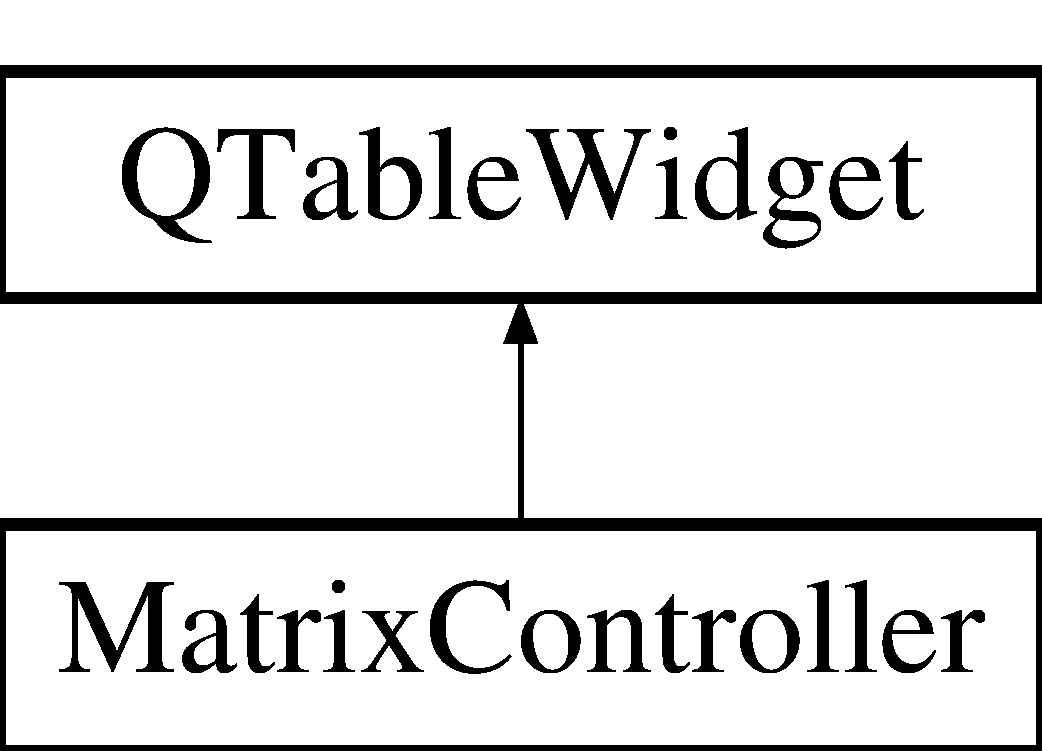
\includegraphics[height=2.000000cm]{class_matrix_controller}
\end{center}
\end{figure}
\subsection*{Public Member Functions}
\begin{DoxyCompactItemize}
\item 
\mbox{\hyperlink{class_matrix_controller_a9b3730013aece0bd3f8cbb28342d091a}{Matrix\+Controller}} (int column, int rows=1, Q\+Widget $\ast$parent=nullptr)
\item 
std\+::vector$<$ bool $>$ \mbox{\hyperlink{class_matrix_controller_a2d83853b18c33b5e9c5d9cda58b69640}{serialize\+Grid}} ()
\item 
std\+::vector$<$ bool $>$ \mbox{\hyperlink{class_matrix_controller_ad746a208e6b2f5ddad05d9da559149d1}{serialize\+Grid}} (bool v)
\item 
void \mbox{\hyperlink{class_matrix_controller_aa2edebadd4baa22559dda6a44a334f7e}{switch\+Bool}} ()
\item 
bool \mbox{\hyperlink{class_matrix_controller_a3dddffef3dba0b1ec308c328c23c2133}{get\+Anim}} () const
\item 
void \mbox{\hyperlink{class_matrix_controller_a9cfa49cb2567dabbf7c333ec7384d15f}{on\+Change\+D1}} (std\+::vector$<$ bool $>$ \&v)
\item 
void \mbox{\hyperlink{class_matrix_controller_a1b0fa2f1568ac4149a27e2695bf55cab}{on\+Change\+D2}} (std\+::vector$<$ bool $>$ \&v)
\item 
void \mbox{\hyperlink{class_matrix_controller_a19a8d008de9323a306daac5aae96ce76}{set\+Dimension}} (\mbox{\hyperlink{automatamanager_8h_ae6fa959b9e8f9c638e0d82bf2c7dc5e7}{dim}} d)
\item 
\mbox{\hyperlink{automatamanager_8h_ae6fa959b9e8f9c638e0d82bf2c7dc5e7}{dim}} \mbox{\hyperlink{class_matrix_controller_a0c6581133615470c77b738737094d7e9}{get\+Dimension}} () const
\end{DoxyCompactItemize}
\subsection*{Private Slots}
\begin{DoxyCompactItemize}
\item 
void \mbox{\hyperlink{class_matrix_controller_a0f75c93c52b1fb1b67af9f9220bfeb22}{on\+Change}} (std\+::vector$<$ bool $>$ \&v)
\item 
void \mbox{\hyperlink{class_matrix_controller_a5cd29184a9f7e7e02a5c3b2baa993aba}{cell\+Activation}} (Q\+Model\+Index)
\end{DoxyCompactItemize}
\subsection*{Private Attributes}
\begin{DoxyCompactItemize}
\item 
Q\+Movie $\ast$ \mbox{\hyperlink{class_matrix_controller_a588c0ffadd7ef176e46d84aaceabd845}{movie}}
\item 
Q\+Movie $\ast$ \mbox{\hyperlink{class_matrix_controller_a61c645ae410eb248913174b116d4f6dd}{movie2}}
\item 
bool \mbox{\hyperlink{class_matrix_controller_a905e5a4996b575460f54f5310ff71c42}{anim}}
\item 
\mbox{\hyperlink{automatamanager_8h_ae6fa959b9e8f9c638e0d82bf2c7dc5e7}{dim}} \mbox{\hyperlink{class_matrix_controller_af09a7f2162eb6086b2269e5d42f8cd5b}{dimension}}
\item 
int \mbox{\hyperlink{class_matrix_controller_a60e65c66b4d68572d47eb1d3b213260a}{index}}
\end{DoxyCompactItemize}
\subsection*{Friends}
\begin{DoxyCompactItemize}
\item 
class \mbox{\hyperlink{class_matrix_controller_a154f5ffe46dc74c6c94311b4cc3927ae}{Main\+Controller}}
\end{DoxyCompactItemize}


\subsection{Constructor \& Destructor Documentation}
\mbox{\Hypertarget{class_matrix_controller_a9b3730013aece0bd3f8cbb28342d091a}\label{class_matrix_controller_a9b3730013aece0bd3f8cbb28342d091a}} 
\index{Matrix\+Controller@{Matrix\+Controller}!Matrix\+Controller@{Matrix\+Controller}}
\index{Matrix\+Controller@{Matrix\+Controller}!Matrix\+Controller@{Matrix\+Controller}}
\subsubsection{\texorpdfstring{Matrix\+Controller()}{MatrixController()}}
{\footnotesize\ttfamily Matrix\+Controller\+::\+Matrix\+Controller (\begin{DoxyParamCaption}\item[{int}]{column,  }\item[{int}]{rows = {\ttfamily 1},  }\item[{Q\+Widget $\ast$}]{parent = {\ttfamily nullptr} }\end{DoxyParamCaption})}



\subsection{Member Function Documentation}
\mbox{\Hypertarget{class_matrix_controller_a5cd29184a9f7e7e02a5c3b2baa993aba}\label{class_matrix_controller_a5cd29184a9f7e7e02a5c3b2baa993aba}} 
\index{Matrix\+Controller@{Matrix\+Controller}!cell\+Activation@{cell\+Activation}}
\index{cell\+Activation@{cell\+Activation}!Matrix\+Controller@{Matrix\+Controller}}
\subsubsection{\texorpdfstring{cell\+Activation}{cellActivation}}
{\footnotesize\ttfamily void Matrix\+Controller\+::cell\+Activation (\begin{DoxyParamCaption}\item[{Q\+Model\+Index}]{index }\end{DoxyParamCaption})\hspace{0.3cm}{\ttfamily [private]}, {\ttfamily [slot]}}

\mbox{\Hypertarget{class_matrix_controller_a3dddffef3dba0b1ec308c328c23c2133}\label{class_matrix_controller_a3dddffef3dba0b1ec308c328c23c2133}} 
\index{Matrix\+Controller@{Matrix\+Controller}!get\+Anim@{get\+Anim}}
\index{get\+Anim@{get\+Anim}!Matrix\+Controller@{Matrix\+Controller}}
\subsubsection{\texorpdfstring{get\+Anim()}{getAnim()}}
{\footnotesize\ttfamily bool Matrix\+Controller\+::get\+Anim (\begin{DoxyParamCaption}{ }\end{DoxyParamCaption}) const\hspace{0.3cm}{\ttfamily [inline]}}

\mbox{\Hypertarget{class_matrix_controller_a0c6581133615470c77b738737094d7e9}\label{class_matrix_controller_a0c6581133615470c77b738737094d7e9}} 
\index{Matrix\+Controller@{Matrix\+Controller}!get\+Dimension@{get\+Dimension}}
\index{get\+Dimension@{get\+Dimension}!Matrix\+Controller@{Matrix\+Controller}}
\subsubsection{\texorpdfstring{get\+Dimension()}{getDimension()}}
{\footnotesize\ttfamily \mbox{\hyperlink{automatamanager_8h_ae6fa959b9e8f9c638e0d82bf2c7dc5e7}{dim}} Matrix\+Controller\+::get\+Dimension (\begin{DoxyParamCaption}{ }\end{DoxyParamCaption}) const\hspace{0.3cm}{\ttfamily [inline]}}

\mbox{\Hypertarget{class_matrix_controller_a0f75c93c52b1fb1b67af9f9220bfeb22}\label{class_matrix_controller_a0f75c93c52b1fb1b67af9f9220bfeb22}} 
\index{Matrix\+Controller@{Matrix\+Controller}!on\+Change@{on\+Change}}
\index{on\+Change@{on\+Change}!Matrix\+Controller@{Matrix\+Controller}}
\subsubsection{\texorpdfstring{on\+Change}{onChange}}
{\footnotesize\ttfamily void Matrix\+Controller\+::on\+Change (\begin{DoxyParamCaption}\item[{std\+::vector$<$ bool $>$ \&}]{v }\end{DoxyParamCaption})\hspace{0.3cm}{\ttfamily [private]}, {\ttfamily [slot]}}

\mbox{\Hypertarget{class_matrix_controller_a9cfa49cb2567dabbf7c333ec7384d15f}\label{class_matrix_controller_a9cfa49cb2567dabbf7c333ec7384d15f}} 
\index{Matrix\+Controller@{Matrix\+Controller}!on\+Change\+D1@{on\+Change\+D1}}
\index{on\+Change\+D1@{on\+Change\+D1}!Matrix\+Controller@{Matrix\+Controller}}
\subsubsection{\texorpdfstring{on\+Change\+D1()}{onChangeD1()}}
{\footnotesize\ttfamily void Matrix\+Controller\+::on\+Change\+D1 (\begin{DoxyParamCaption}\item[{std\+::vector$<$ bool $>$ \&}]{v }\end{DoxyParamCaption})}

\mbox{\Hypertarget{class_matrix_controller_a1b0fa2f1568ac4149a27e2695bf55cab}\label{class_matrix_controller_a1b0fa2f1568ac4149a27e2695bf55cab}} 
\index{Matrix\+Controller@{Matrix\+Controller}!on\+Change\+D2@{on\+Change\+D2}}
\index{on\+Change\+D2@{on\+Change\+D2}!Matrix\+Controller@{Matrix\+Controller}}
\subsubsection{\texorpdfstring{on\+Change\+D2()}{onChangeD2()}}
{\footnotesize\ttfamily void Matrix\+Controller\+::on\+Change\+D2 (\begin{DoxyParamCaption}\item[{std\+::vector$<$ bool $>$ \&}]{v }\end{DoxyParamCaption})}

\mbox{\Hypertarget{class_matrix_controller_a2d83853b18c33b5e9c5d9cda58b69640}\label{class_matrix_controller_a2d83853b18c33b5e9c5d9cda58b69640}} 
\index{Matrix\+Controller@{Matrix\+Controller}!serialize\+Grid@{serialize\+Grid}}
\index{serialize\+Grid@{serialize\+Grid}!Matrix\+Controller@{Matrix\+Controller}}
\subsubsection{\texorpdfstring{serialize\+Grid()}{serializeGrid()}\hspace{0.1cm}{\footnotesize\ttfamily [1/2]}}
{\footnotesize\ttfamily std\+::vector$<$ bool $>$ Matrix\+Controller\+::serialize\+Grid (\begin{DoxyParamCaption}{ }\end{DoxyParamCaption})}

\mbox{\Hypertarget{class_matrix_controller_ad746a208e6b2f5ddad05d9da559149d1}\label{class_matrix_controller_ad746a208e6b2f5ddad05d9da559149d1}} 
\index{Matrix\+Controller@{Matrix\+Controller}!serialize\+Grid@{serialize\+Grid}}
\index{serialize\+Grid@{serialize\+Grid}!Matrix\+Controller@{Matrix\+Controller}}
\subsubsection{\texorpdfstring{serialize\+Grid()}{serializeGrid()}\hspace{0.1cm}{\footnotesize\ttfamily [2/2]}}
{\footnotesize\ttfamily std\+::vector$<$ bool $>$ Matrix\+Controller\+::serialize\+Grid (\begin{DoxyParamCaption}\item[{bool}]{v }\end{DoxyParamCaption})}

\mbox{\Hypertarget{class_matrix_controller_a19a8d008de9323a306daac5aae96ce76}\label{class_matrix_controller_a19a8d008de9323a306daac5aae96ce76}} 
\index{Matrix\+Controller@{Matrix\+Controller}!set\+Dimension@{set\+Dimension}}
\index{set\+Dimension@{set\+Dimension}!Matrix\+Controller@{Matrix\+Controller}}
\subsubsection{\texorpdfstring{set\+Dimension()}{setDimension()}}
{\footnotesize\ttfamily void Matrix\+Controller\+::set\+Dimension (\begin{DoxyParamCaption}\item[{\mbox{\hyperlink{automatamanager_8h_ae6fa959b9e8f9c638e0d82bf2c7dc5e7}{dim}}}]{d }\end{DoxyParamCaption})\hspace{0.3cm}{\ttfamily [inline]}}

\mbox{\Hypertarget{class_matrix_controller_aa2edebadd4baa22559dda6a44a334f7e}\label{class_matrix_controller_aa2edebadd4baa22559dda6a44a334f7e}} 
\index{Matrix\+Controller@{Matrix\+Controller}!switch\+Bool@{switch\+Bool}}
\index{switch\+Bool@{switch\+Bool}!Matrix\+Controller@{Matrix\+Controller}}
\subsubsection{\texorpdfstring{switch\+Bool()}{switchBool()}}
{\footnotesize\ttfamily void Matrix\+Controller\+::switch\+Bool (\begin{DoxyParamCaption}{ }\end{DoxyParamCaption})\hspace{0.3cm}{\ttfamily [inline]}}



\subsection{Friends And Related Function Documentation}
\mbox{\Hypertarget{class_matrix_controller_a154f5ffe46dc74c6c94311b4cc3927ae}\label{class_matrix_controller_a154f5ffe46dc74c6c94311b4cc3927ae}} 
\index{Matrix\+Controller@{Matrix\+Controller}!Main\+Controller@{Main\+Controller}}
\index{Main\+Controller@{Main\+Controller}!Matrix\+Controller@{Matrix\+Controller}}
\subsubsection{\texorpdfstring{Main\+Controller}{MainController}}
{\footnotesize\ttfamily friend class \mbox{\hyperlink{class_main_controller}{Main\+Controller}}\hspace{0.3cm}{\ttfamily [friend]}}



\subsection{Member Data Documentation}
\mbox{\Hypertarget{class_matrix_controller_a905e5a4996b575460f54f5310ff71c42}\label{class_matrix_controller_a905e5a4996b575460f54f5310ff71c42}} 
\index{Matrix\+Controller@{Matrix\+Controller}!anim@{anim}}
\index{anim@{anim}!Matrix\+Controller@{Matrix\+Controller}}
\subsubsection{\texorpdfstring{anim}{anim}}
{\footnotesize\ttfamily bool Matrix\+Controller\+::anim\hspace{0.3cm}{\ttfamily [private]}}

\mbox{\Hypertarget{class_matrix_controller_af09a7f2162eb6086b2269e5d42f8cd5b}\label{class_matrix_controller_af09a7f2162eb6086b2269e5d42f8cd5b}} 
\index{Matrix\+Controller@{Matrix\+Controller}!dimension@{dimension}}
\index{dimension@{dimension}!Matrix\+Controller@{Matrix\+Controller}}
\subsubsection{\texorpdfstring{dimension}{dimension}}
{\footnotesize\ttfamily \mbox{\hyperlink{automatamanager_8h_ae6fa959b9e8f9c638e0d82bf2c7dc5e7}{dim}} Matrix\+Controller\+::dimension\hspace{0.3cm}{\ttfamily [private]}}

\mbox{\Hypertarget{class_matrix_controller_a60e65c66b4d68572d47eb1d3b213260a}\label{class_matrix_controller_a60e65c66b4d68572d47eb1d3b213260a}} 
\index{Matrix\+Controller@{Matrix\+Controller}!index@{index}}
\index{index@{index}!Matrix\+Controller@{Matrix\+Controller}}
\subsubsection{\texorpdfstring{index}{index}}
{\footnotesize\ttfamily int Matrix\+Controller\+::index\hspace{0.3cm}{\ttfamily [private]}}

\mbox{\Hypertarget{class_matrix_controller_a588c0ffadd7ef176e46d84aaceabd845}\label{class_matrix_controller_a588c0ffadd7ef176e46d84aaceabd845}} 
\index{Matrix\+Controller@{Matrix\+Controller}!movie@{movie}}
\index{movie@{movie}!Matrix\+Controller@{Matrix\+Controller}}
\subsubsection{\texorpdfstring{movie}{movie}}
{\footnotesize\ttfamily Q\+Movie$\ast$ Matrix\+Controller\+::movie\hspace{0.3cm}{\ttfamily [private]}}

\mbox{\Hypertarget{class_matrix_controller_a61c645ae410eb248913174b116d4f6dd}\label{class_matrix_controller_a61c645ae410eb248913174b116d4f6dd}} 
\index{Matrix\+Controller@{Matrix\+Controller}!movie2@{movie2}}
\index{movie2@{movie2}!Matrix\+Controller@{Matrix\+Controller}}
\subsubsection{\texorpdfstring{movie2}{movie2}}
{\footnotesize\ttfamily Q\+Movie$\ast$ Matrix\+Controller\+::movie2\hspace{0.3cm}{\ttfamily [private]}}



The documentation for this class was generated from the following files\+:\begin{DoxyCompactItemize}
\item 
\mbox{\hyperlink{matrixcontroller_8h}{matrixcontroller.\+h}}\item 
\mbox{\hyperlink{matrixcontroller_8cpp}{matrixcontroller.\+cpp}}\end{DoxyCompactItemize}

\hypertarget{class_neighbour_rule}{}\section{Neighbour\+Rule Class Reference}
\label{class_neighbour_rule}\index{Neighbour\+Rule@{Neighbour\+Rule}}


{\ttfamily \#include $<$rulescontroller.\+h$>$}

Inheritance diagram for Neighbour\+Rule\+:\begin{figure}[H]
\begin{center}
\leavevmode
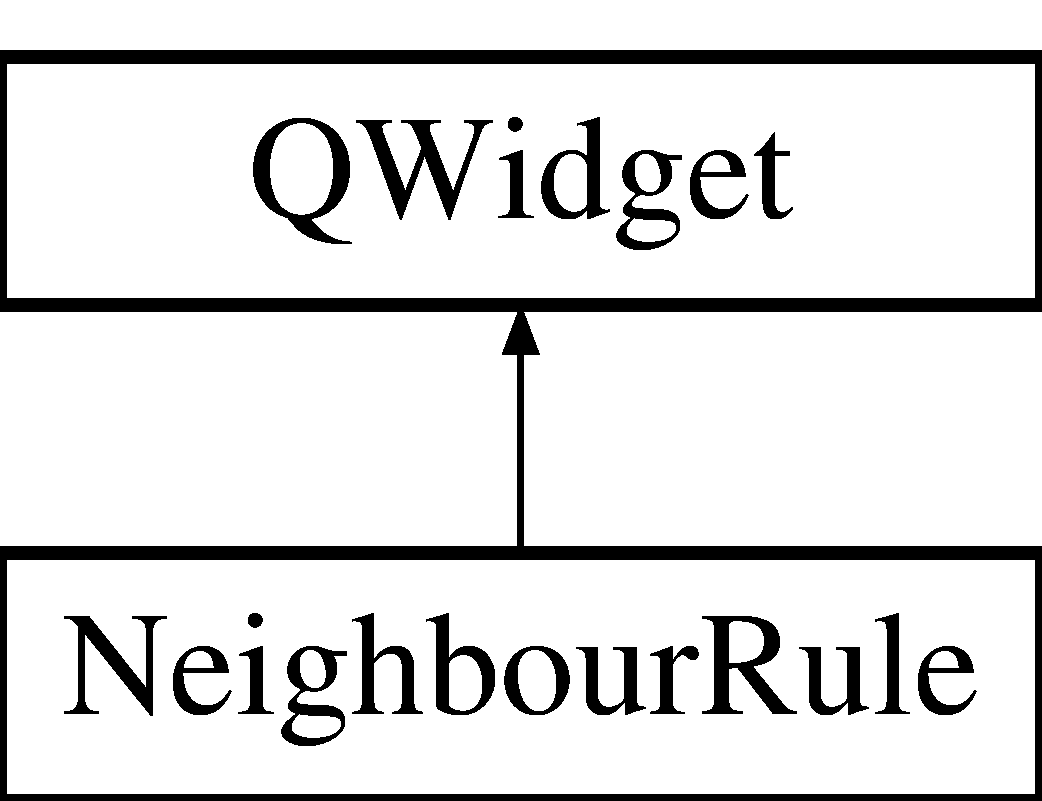
\includegraphics[height=2.000000cm]{class_neighbour_rule}
\end{center}
\end{figure}
\subsection*{Public Member Functions}
\begin{DoxyCompactItemize}
\item 
\mbox{\hyperlink{class_neighbour_rule_ab9bd69920202b3826ea959ec5b309fe0}{Neighbour\+Rule}} (int N, Q\+Widget $\ast$parent=nullptr)
\end{DoxyCompactItemize}
\subsection*{Private Attributes}
\begin{DoxyCompactItemize}
\item 
Q\+Spin\+Box $\ast$ \mbox{\hyperlink{class_neighbour_rule_aa0dd87a547aa630fc741bcd1ed7c3007}{from}}
\item 
Q\+Spin\+Box $\ast$ \mbox{\hyperlink{class_neighbour_rule_a9fd5cf760c4ccfeefb104f24e6488a51}{to}}
\item 
Q\+Check\+Box $\ast$ \mbox{\hyperlink{class_neighbour_rule_a55af8eae63687835de271eee068732ce}{min}}
\item 
Q\+Push\+Button $\ast$ \mbox{\hyperlink{class_neighbour_rule_ab62a36811d4af2b13f7d25820a8eaab6}{max}}
\end{DoxyCompactItemize}
\subsection*{Friends}
\begin{DoxyCompactItemize}
\item 
class \mbox{\hyperlink{class_neighbour_rule_a4a3b7cfb8cbef548cad1c2c16c6ce941}{Rules\+Controller}}
\item 
class \mbox{\hyperlink{class_neighbour_rule_a154f5ffe46dc74c6c94311b4cc3927ae}{Main\+Controller}}
\end{DoxyCompactItemize}


\subsection{Constructor \& Destructor Documentation}
\mbox{\Hypertarget{class_neighbour_rule_ab9bd69920202b3826ea959ec5b309fe0}\label{class_neighbour_rule_ab9bd69920202b3826ea959ec5b309fe0}} 
\index{Neighbour\+Rule@{Neighbour\+Rule}!Neighbour\+Rule@{Neighbour\+Rule}}
\index{Neighbour\+Rule@{Neighbour\+Rule}!Neighbour\+Rule@{Neighbour\+Rule}}
\subsubsection{\texorpdfstring{Neighbour\+Rule()}{NeighbourRule()}}
{\footnotesize\ttfamily Neighbour\+Rule\+::\+Neighbour\+Rule (\begin{DoxyParamCaption}\item[{int}]{N,  }\item[{Q\+Widget $\ast$}]{parent = {\ttfamily nullptr} }\end{DoxyParamCaption})\hspace{0.3cm}{\ttfamily [explicit]}}



\subsection{Friends And Related Function Documentation}
\mbox{\Hypertarget{class_neighbour_rule_a154f5ffe46dc74c6c94311b4cc3927ae}\label{class_neighbour_rule_a154f5ffe46dc74c6c94311b4cc3927ae}} 
\index{Neighbour\+Rule@{Neighbour\+Rule}!Main\+Controller@{Main\+Controller}}
\index{Main\+Controller@{Main\+Controller}!Neighbour\+Rule@{Neighbour\+Rule}}
\subsubsection{\texorpdfstring{Main\+Controller}{MainController}}
{\footnotesize\ttfamily friend class \mbox{\hyperlink{class_main_controller}{Main\+Controller}}\hspace{0.3cm}{\ttfamily [friend]}}

\mbox{\Hypertarget{class_neighbour_rule_a4a3b7cfb8cbef548cad1c2c16c6ce941}\label{class_neighbour_rule_a4a3b7cfb8cbef548cad1c2c16c6ce941}} 
\index{Neighbour\+Rule@{Neighbour\+Rule}!Rules\+Controller@{Rules\+Controller}}
\index{Rules\+Controller@{Rules\+Controller}!Neighbour\+Rule@{Neighbour\+Rule}}
\subsubsection{\texorpdfstring{Rules\+Controller}{RulesController}}
{\footnotesize\ttfamily friend class \mbox{\hyperlink{class_rules_controller}{Rules\+Controller}}\hspace{0.3cm}{\ttfamily [friend]}}



\subsection{Member Data Documentation}
\mbox{\Hypertarget{class_neighbour_rule_aa0dd87a547aa630fc741bcd1ed7c3007}\label{class_neighbour_rule_aa0dd87a547aa630fc741bcd1ed7c3007}} 
\index{Neighbour\+Rule@{Neighbour\+Rule}!from@{from}}
\index{from@{from}!Neighbour\+Rule@{Neighbour\+Rule}}
\subsubsection{\texorpdfstring{from}{from}}
{\footnotesize\ttfamily Q\+Spin\+Box$\ast$ Neighbour\+Rule\+::from\hspace{0.3cm}{\ttfamily [private]}}

\mbox{\Hypertarget{class_neighbour_rule_ab62a36811d4af2b13f7d25820a8eaab6}\label{class_neighbour_rule_ab62a36811d4af2b13f7d25820a8eaab6}} 
\index{Neighbour\+Rule@{Neighbour\+Rule}!max@{max}}
\index{max@{max}!Neighbour\+Rule@{Neighbour\+Rule}}
\subsubsection{\texorpdfstring{max}{max}}
{\footnotesize\ttfamily Q\+Push\+Button$\ast$ Neighbour\+Rule\+::max\hspace{0.3cm}{\ttfamily [private]}}

\mbox{\Hypertarget{class_neighbour_rule_a55af8eae63687835de271eee068732ce}\label{class_neighbour_rule_a55af8eae63687835de271eee068732ce}} 
\index{Neighbour\+Rule@{Neighbour\+Rule}!min@{min}}
\index{min@{min}!Neighbour\+Rule@{Neighbour\+Rule}}
\subsubsection{\texorpdfstring{min}{min}}
{\footnotesize\ttfamily Q\+Check\+Box$\ast$ Neighbour\+Rule\+::min\hspace{0.3cm}{\ttfamily [private]}}

\mbox{\Hypertarget{class_neighbour_rule_a9fd5cf760c4ccfeefb104f24e6488a51}\label{class_neighbour_rule_a9fd5cf760c4ccfeefb104f24e6488a51}} 
\index{Neighbour\+Rule@{Neighbour\+Rule}!to@{to}}
\index{to@{to}!Neighbour\+Rule@{Neighbour\+Rule}}
\subsubsection{\texorpdfstring{to}{to}}
{\footnotesize\ttfamily Q\+Spin\+Box$\ast$ Neighbour\+Rule\+::to\hspace{0.3cm}{\ttfamily [private]}}



The documentation for this class was generated from the following files\+:\begin{DoxyCompactItemize}
\item 
\mbox{\hyperlink{rulescontroller_8h}{rulescontroller.\+h}}\item 
\mbox{\hyperlink{rulescontroller_8cpp}{rulescontroller.\+cpp}}\end{DoxyCompactItemize}

\hypertarget{class_position_rule}{}\section{Position\+Rule Class Reference}
\label{class_position_rule}\index{Position\+Rule@{Position\+Rule}}


{\ttfamily \#include $<$rulescontroller.\+h$>$}

Inheritance diagram for Position\+Rule\+:\begin{figure}[H]
\begin{center}
\leavevmode
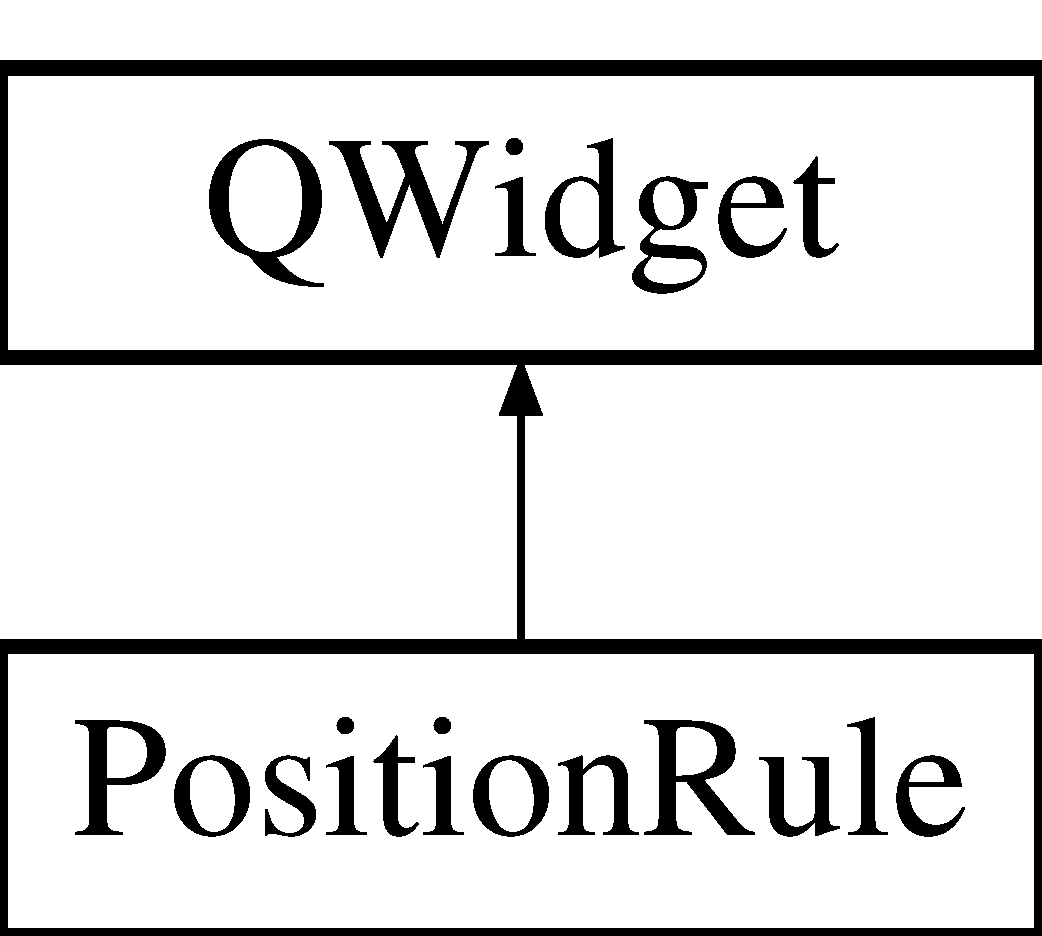
\includegraphics[height=2.000000cm]{class_position_rule}
\end{center}
\end{figure}
\subsection*{Public Member Functions}
\begin{DoxyCompactItemize}
\item 
\mbox{\hyperlink{class_position_rule_a5db88bbd487ea356486bf5e3183f3c81}{Position\+Rule}} (int column, int rows=1, Q\+Widget $\ast$parent=nullptr)
\end{DoxyCompactItemize}
\subsection*{Private Attributes}
\begin{DoxyCompactItemize}
\item 
\mbox{\hyperlink{class_matrix_controller}{Matrix\+Controller}} $\ast$ \mbox{\hyperlink{class_position_rule_a1b8c45dd4a95666a2f1826a063fba837}{position\+Matrix}}
\end{DoxyCompactItemize}
\subsection*{Friends}
\begin{DoxyCompactItemize}
\item 
class \mbox{\hyperlink{class_position_rule_a154f5ffe46dc74c6c94311b4cc3927ae}{Main\+Controller}}
\end{DoxyCompactItemize}


\subsection{Constructor \& Destructor Documentation}
\mbox{\Hypertarget{class_position_rule_a5db88bbd487ea356486bf5e3183f3c81}\label{class_position_rule_a5db88bbd487ea356486bf5e3183f3c81}} 
\index{Position\+Rule@{Position\+Rule}!Position\+Rule@{Position\+Rule}}
\index{Position\+Rule@{Position\+Rule}!Position\+Rule@{Position\+Rule}}
\subsubsection{\texorpdfstring{Position\+Rule()}{PositionRule()}}
{\footnotesize\ttfamily Position\+Rule\+::\+Position\+Rule (\begin{DoxyParamCaption}\item[{int}]{column,  }\item[{int}]{rows = {\ttfamily 1},  }\item[{Q\+Widget $\ast$}]{parent = {\ttfamily nullptr} }\end{DoxyParamCaption})\hspace{0.3cm}{\ttfamily [explicit]}}



\subsection{Friends And Related Function Documentation}
\mbox{\Hypertarget{class_position_rule_a154f5ffe46dc74c6c94311b4cc3927ae}\label{class_position_rule_a154f5ffe46dc74c6c94311b4cc3927ae}} 
\index{Position\+Rule@{Position\+Rule}!Main\+Controller@{Main\+Controller}}
\index{Main\+Controller@{Main\+Controller}!Position\+Rule@{Position\+Rule}}
\subsubsection{\texorpdfstring{Main\+Controller}{MainController}}
{\footnotesize\ttfamily friend class \mbox{\hyperlink{class_main_controller}{Main\+Controller}}\hspace{0.3cm}{\ttfamily [friend]}}



\subsection{Member Data Documentation}
\mbox{\Hypertarget{class_position_rule_a1b8c45dd4a95666a2f1826a063fba837}\label{class_position_rule_a1b8c45dd4a95666a2f1826a063fba837}} 
\index{Position\+Rule@{Position\+Rule}!position\+Matrix@{position\+Matrix}}
\index{position\+Matrix@{position\+Matrix}!Position\+Rule@{Position\+Rule}}
\subsubsection{\texorpdfstring{position\+Matrix}{positionMatrix}}
{\footnotesize\ttfamily \mbox{\hyperlink{class_matrix_controller}{Matrix\+Controller}}$\ast$ Position\+Rule\+::position\+Matrix\hspace{0.3cm}{\ttfamily [private]}}



The documentation for this class was generated from the following files\+:\begin{DoxyCompactItemize}
\item 
\mbox{\hyperlink{rulescontroller_8h}{rulescontroller.\+h}}\item 
\mbox{\hyperlink{rulescontroller_8cpp}{rulescontroller.\+cpp}}\end{DoxyCompactItemize}

\hypertarget{struct_automaton_1_1_range}{}\section{Automaton\+:\+:Range Struct Reference}
\label{struct_automaton_1_1_range}\index{Automaton\+::\+Range@{Automaton\+::\+Range}}


Permet de stocker un intervalle.  


\subsection*{Public Attributes}
\begin{DoxyCompactItemize}
\item 
unsigned int \mbox{\hyperlink{struct_automaton_1_1_range_a95a564b78f9913c5c0bf955a67dd4e5b}{a}}
\item 
unsigned int \mbox{\hyperlink{struct_automaton_1_1_range_a64572f881a1cde5248ff57efdcf073af}{b}}
\end{DoxyCompactItemize}


\subsection{Detailed Description}
Permet de stocker un intervalle. 

\subsection{Member Data Documentation}
\mbox{\Hypertarget{struct_automaton_1_1_range_a95a564b78f9913c5c0bf955a67dd4e5b}\label{struct_automaton_1_1_range_a95a564b78f9913c5c0bf955a67dd4e5b}} 
\index{Automaton\+::\+Range@{Automaton\+::\+Range}!a@{a}}
\index{a@{a}!Automaton\+::\+Range@{Automaton\+::\+Range}}
\subsubsection{\texorpdfstring{a}{a}}
{\footnotesize\ttfamily unsigned int Automaton\+::\+Range\+::a}

\mbox{\Hypertarget{struct_automaton_1_1_range_a64572f881a1cde5248ff57efdcf073af}\label{struct_automaton_1_1_range_a64572f881a1cde5248ff57efdcf073af}} 
\index{Automaton\+::\+Range@{Automaton\+::\+Range}!b@{b}}
\index{b@{b}!Automaton\+::\+Range@{Automaton\+::\+Range}}
\subsubsection{\texorpdfstring{b}{b}}
{\footnotesize\ttfamily unsigned int Automaton\+::\+Range\+::b}



The documentation for this struct was generated from the following file\+:\begin{DoxyCompactItemize}
\item 
\mbox{\hyperlink{automaton_8h}{automaton.\+h}}\end{DoxyCompactItemize}

\hypertarget{class_rules_controller}{}\section{Rules\+Controller Class Reference}
\label{class_rules_controller}\index{Rules\+Controller@{Rules\+Controller}}


{\ttfamily \#include $<$rulescontroller.\+h$>$}

Inheritance diagram for Rules\+Controller\+:\begin{figure}[H]
\begin{center}
\leavevmode
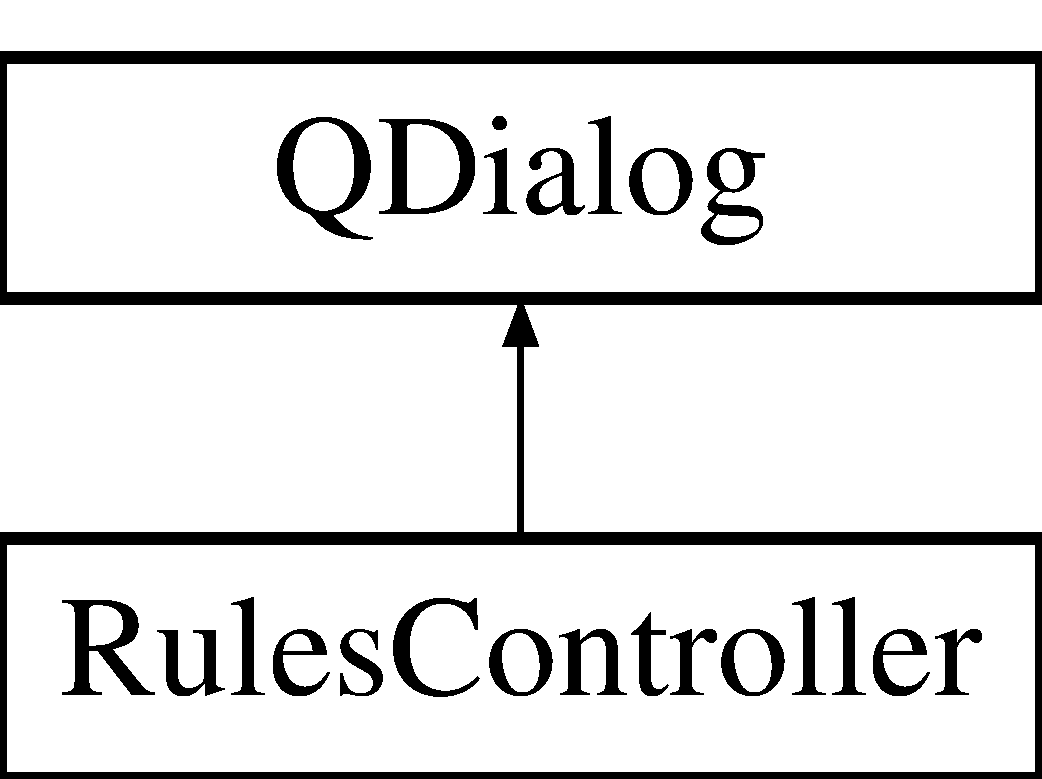
\includegraphics[height=2.000000cm]{class_rules_controller}
\end{center}
\end{figure}
\subsection*{Public Member Functions}
\begin{DoxyCompactItemize}
\item 
\mbox{\hyperlink{class_rules_controller_a91f872c80e266517c4fd12674b477996}{Rules\+Controller}} (char def, int N, int column, int row=1, Q\+Widget $\ast$parent=0)
\end{DoxyCompactItemize}
\subsection*{Private Attributes}
\begin{DoxyCompactItemize}
\item 
Q\+Tab\+Widget $\ast$ \mbox{\hyperlink{class_rules_controller_afcb40145540839909f809fe27d24156c}{tab\+Widget}}
\item 
Q\+Dialog\+Button\+Box $\ast$ \mbox{\hyperlink{class_rules_controller_a53f287abf68fb9891bdd7a6f21f31c22}{button\+Box}}
\item 
Q\+Radio\+Button $\ast$ \mbox{\hyperlink{class_rules_controller_a2f993272d5b1faac4f52116d6e66afbf}{dead}}
\item 
Q\+Radio\+Button $\ast$ \mbox{\hyperlink{class_rules_controller_a24a431e369285ef2cf12a95eeeb0c7e1}{alive}}
\item 
Q\+Radio\+Button $\ast$ \mbox{\hyperlink{class_rules_controller_afee85c960a94ec09c46e74036cfbb81b}{same}}
\end{DoxyCompactItemize}
\subsection*{Friends}
\begin{DoxyCompactItemize}
\item 
class \mbox{\hyperlink{class_rules_controller_a154f5ffe46dc74c6c94311b4cc3927ae}{Main\+Controller}}
\end{DoxyCompactItemize}


\subsection{Constructor \& Destructor Documentation}
\mbox{\Hypertarget{class_rules_controller_a91f872c80e266517c4fd12674b477996}\label{class_rules_controller_a91f872c80e266517c4fd12674b477996}} 
\index{Rules\+Controller@{Rules\+Controller}!Rules\+Controller@{Rules\+Controller}}
\index{Rules\+Controller@{Rules\+Controller}!Rules\+Controller@{Rules\+Controller}}
\subsubsection{\texorpdfstring{Rules\+Controller()}{RulesController()}}
{\footnotesize\ttfamily Rules\+Controller\+::\+Rules\+Controller (\begin{DoxyParamCaption}\item[{char}]{def,  }\item[{int}]{N,  }\item[{int}]{column,  }\item[{int}]{row = {\ttfamily 1},  }\item[{Q\+Widget $\ast$}]{parent = {\ttfamily 0} }\end{DoxyParamCaption})}



\subsection{Friends And Related Function Documentation}
\mbox{\Hypertarget{class_rules_controller_a154f5ffe46dc74c6c94311b4cc3927ae}\label{class_rules_controller_a154f5ffe46dc74c6c94311b4cc3927ae}} 
\index{Rules\+Controller@{Rules\+Controller}!Main\+Controller@{Main\+Controller}}
\index{Main\+Controller@{Main\+Controller}!Rules\+Controller@{Rules\+Controller}}
\subsubsection{\texorpdfstring{Main\+Controller}{MainController}}
{\footnotesize\ttfamily friend class \mbox{\hyperlink{class_main_controller}{Main\+Controller}}\hspace{0.3cm}{\ttfamily [friend]}}



\subsection{Member Data Documentation}
\mbox{\Hypertarget{class_rules_controller_a24a431e369285ef2cf12a95eeeb0c7e1}\label{class_rules_controller_a24a431e369285ef2cf12a95eeeb0c7e1}} 
\index{Rules\+Controller@{Rules\+Controller}!alive@{alive}}
\index{alive@{alive}!Rules\+Controller@{Rules\+Controller}}
\subsubsection{\texorpdfstring{alive}{alive}}
{\footnotesize\ttfamily Q\+Radio\+Button$\ast$ Rules\+Controller\+::alive\hspace{0.3cm}{\ttfamily [private]}}

\mbox{\Hypertarget{class_rules_controller_a53f287abf68fb9891bdd7a6f21f31c22}\label{class_rules_controller_a53f287abf68fb9891bdd7a6f21f31c22}} 
\index{Rules\+Controller@{Rules\+Controller}!button\+Box@{button\+Box}}
\index{button\+Box@{button\+Box}!Rules\+Controller@{Rules\+Controller}}
\subsubsection{\texorpdfstring{button\+Box}{buttonBox}}
{\footnotesize\ttfamily Q\+Dialog\+Button\+Box$\ast$ Rules\+Controller\+::button\+Box\hspace{0.3cm}{\ttfamily [private]}}

\mbox{\Hypertarget{class_rules_controller_a2f993272d5b1faac4f52116d6e66afbf}\label{class_rules_controller_a2f993272d5b1faac4f52116d6e66afbf}} 
\index{Rules\+Controller@{Rules\+Controller}!dead@{dead}}
\index{dead@{dead}!Rules\+Controller@{Rules\+Controller}}
\subsubsection{\texorpdfstring{dead}{dead}}
{\footnotesize\ttfamily Q\+Radio\+Button$\ast$ Rules\+Controller\+::dead\hspace{0.3cm}{\ttfamily [private]}}

\mbox{\Hypertarget{class_rules_controller_afee85c960a94ec09c46e74036cfbb81b}\label{class_rules_controller_afee85c960a94ec09c46e74036cfbb81b}} 
\index{Rules\+Controller@{Rules\+Controller}!same@{same}}
\index{same@{same}!Rules\+Controller@{Rules\+Controller}}
\subsubsection{\texorpdfstring{same}{same}}
{\footnotesize\ttfamily Q\+Radio\+Button$\ast$ Rules\+Controller\+::same\hspace{0.3cm}{\ttfamily [private]}}

\mbox{\Hypertarget{class_rules_controller_afcb40145540839909f809fe27d24156c}\label{class_rules_controller_afcb40145540839909f809fe27d24156c}} 
\index{Rules\+Controller@{Rules\+Controller}!tab\+Widget@{tab\+Widget}}
\index{tab\+Widget@{tab\+Widget}!Rules\+Controller@{Rules\+Controller}}
\subsubsection{\texorpdfstring{tab\+Widget}{tabWidget}}
{\footnotesize\ttfamily Q\+Tab\+Widget$\ast$ Rules\+Controller\+::tab\+Widget\hspace{0.3cm}{\ttfamily [private]}}



The documentation for this class was generated from the following files\+:\begin{DoxyCompactItemize}
\item 
\mbox{\hyperlink{rulescontroller_8h}{rulescontroller.\+h}}\item 
\mbox{\hyperlink{rulescontroller_8cpp}{rulescontroller.\+cpp}}\end{DoxyCompactItemize}

\hypertarget{class_state}{}\section{State Class Reference}
\label{class_state}\index{State@{State}}


{\ttfamily \#include $<$state.\+h$>$}

Inheritance diagram for State\+:\begin{figure}[H]
\begin{center}
\leavevmode
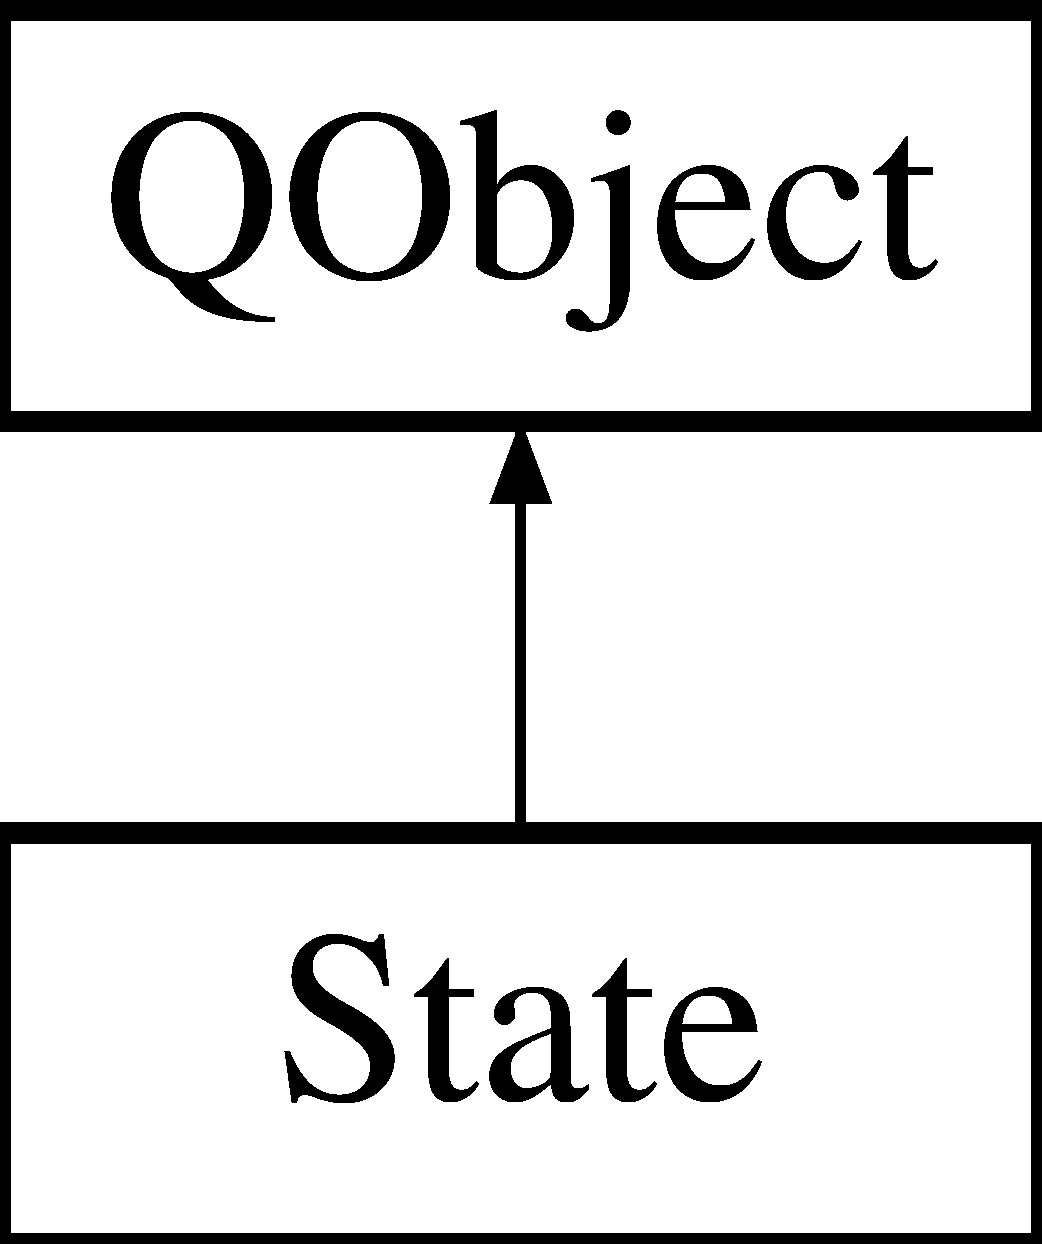
\includegraphics[height=2.000000cm]{class_state}
\end{center}
\end{figure}
\subsection*{Signals}
\begin{DoxyCompactItemize}
\item 
void \mbox{\hyperlink{class_state_a7a3e3dd36808cc394e8514902d55b856}{value\+Changed}} (std\+::vector$<$ bool $>$ \&)
\begin{DoxyCompactList}\small\item\em Signal qui sera envoyé à la vue lorsque state est modifié \end{DoxyCompactList}\end{DoxyCompactItemize}
\subsection*{Public Member Functions}
\begin{DoxyCompactItemize}
\item 
Q\+String \mbox{\hyperlink{class_state_aeadbbdbf52ed603425180ccb53d841cd}{to\+String}} () const
\begin{DoxyCompactList}\small\item\em méthode de sérialisation du vecteur state \end{DoxyCompactList}\item 
\mbox{\hyperlink{class_state_a66c925e564c8e29814ec8519e90fdf90}{State}} (\mbox{\hyperlink{class_state}{State}} const \&old)
\begin{DoxyCompactList}\small\item\em Constructeur de recopie. \end{DoxyCompactList}\item 
\mbox{\hyperlink{class_state_aed4ab30fe127984d9d7f1327abd50976}{State}} (Q\+String const \&file\+Name)
\begin{DoxyCompactList}\small\item\em Constructeur à partir d\textquotesingle{}un fichier. \end{DoxyCompactList}\item 
\mbox{\hyperlink{class_state_a8c645ab945f02b1c90b814ebb67bfcc3}{State}} (const \mbox{\hyperlink{state_8h_a4840c4503b7d10cea5e08416eb3716f1}{Uint}} id, sqlite3 $\ast$db)
\begin{DoxyCompactList}\small\item\em Constructeur à partir d\textquotesingle{}\textquotesingle{}un automate de la B\+DD. \end{DoxyCompactList}\item 
\mbox{\hyperlink{class_state_a647bdb0ebd9012e00ce54400dbb247f0}{State}} (const \mbox{\hyperlink{state_8h_a4840c4503b7d10cea5e08416eb3716f1}{Uint}} dimension1d)
\begin{DoxyCompactList}\small\item\em Constructeur d\textquotesingle{}état 1D aléatoire. \end{DoxyCompactList}\item 
\mbox{\hyperlink{class_state_af599b90d950b89a489ac23a584b1c0e3}{State}} (const \mbox{\hyperlink{state_8h_a4840c4503b7d10cea5e08416eb3716f1}{Uint}} dimension1d, \mbox{\hyperlink{state_8h_aa074fbe250e9d18fbe221bb7473158ad}{Vec}} v)
\begin{DoxyCompactList}\small\item\em Constructeur d\textquotesingle{}état 1D non-\/aléatoire. \end{DoxyCompactList}\item 
\mbox{\hyperlink{class_state_a72792193d86ae159600a31bf40dd3912}{State}} (const \mbox{\hyperlink{state_8h_a4840c4503b7d10cea5e08416eb3716f1}{Uint}} row\+Dimension, const \mbox{\hyperlink{state_8h_a4840c4503b7d10cea5e08416eb3716f1}{Uint}} col\+Dimension)
\begin{DoxyCompactList}\small\item\em Constructeur d\textquotesingle{}état 2D aléatoire. \end{DoxyCompactList}\item 
\mbox{\hyperlink{class_state_a0fd7e27557fffb01934f86ae99720e9e}{State}} (const \mbox{\hyperlink{state_8h_a4840c4503b7d10cea5e08416eb3716f1}{Uint}} row\+Dimension, const \mbox{\hyperlink{state_8h_a4840c4503b7d10cea5e08416eb3716f1}{Uint}} col\+Dimension, \mbox{\hyperlink{state_8h_aa074fbe250e9d18fbe221bb7473158ad}{Vec}} v)
\begin{DoxyCompactList}\small\item\em Constructeur d\textquotesingle{}état 2D non-\/aléatoire. \end{DoxyCompactList}\item 
\mbox{\hyperlink{state_8h_a4840c4503b7d10cea5e08416eb3716f1}{Uint}} \mbox{\hyperlink{class_state_a7897325c49eb83639365bc61d806fab2}{get\+Nrow}} () const
\item 
\mbox{\hyperlink{state_8h_a4840c4503b7d10cea5e08416eb3716f1}{Uint}} \mbox{\hyperlink{class_state_a706098b5c48bcf68bfb3a8676bb5a868}{get\+Ncol}} () const
\item 
const \mbox{\hyperlink{state_8h_aa074fbe250e9d18fbe221bb7473158ad}{Vec}} \& \mbox{\hyperlink{class_state_aa2168c5a262b6bce4cbadc069d72d1be}{get\+State}} () const
\item 
void \mbox{\hyperlink{class_state_ad3c992e4b6e2e857f8f261575d37c3c4}{set\+State}} (\mbox{\hyperlink{state_8h_aa074fbe250e9d18fbe221bb7473158ad}{Vec}} \&v)
\item 
void \mbox{\hyperlink{class_state_a7f9db12892f20438c4e00796e28a0dac}{emit\+Signal}} ()
\begin{DoxyCompactList}\small\item\em Permet d\textquotesingle{}émettre le signal value\+Changd, envoyant une référence de state. \end{DoxyCompactList}\item 
void \mbox{\hyperlink{class_state_ae51e526916dea6aa33f0dbd4529f877b}{random\+State}} ()
\begin{DoxyCompactList}\small\item\em Rempli state de manière aléatoire. \end{DoxyCompactList}\item 
\mbox{\hyperlink{state_8h_a4840c4503b7d10cea5e08416eb3716f1}{Uint}} \mbox{\hyperlink{class_state_adcb67718b6f2502d7e4e150a18a5bf0b}{save}} (const Q\+String \&name, sqlite3 $\ast$db) const
\begin{DoxyCompactList}\small\item\em Sauvegarde l\textquotesingle{}état dans la B\+DD. \end{DoxyCompactList}\item 
void \mbox{\hyperlink{class_state_a7dfee0c004e500cca7f050e800daefcf}{export\+To\+File}} (Q\+String const \&name) const
\begin{DoxyCompactList}\small\item\em Exporte l\textquotesingle{}état dans un fichier. \end{DoxyCompactList}\item 
std\+::vector$<$ std\+::string $>$ \mbox{\hyperlink{class_state_a9681c4601cfbcd05f9c203770105bd1e}{stack\+Of\+Nb}} (\mbox{\hyperlink{state_8h_a4840c4503b7d10cea5e08416eb3716f1}{Uint}} n) const
\begin{DoxyCompactList}\small\item\em Permet d\textquotesingle{}envoyer les voisins significatifs de chaque case. \end{DoxyCompactList}\end{DoxyCompactItemize}
\subsection*{Private Member Functions}
\begin{DoxyCompactItemize}
\item 
void \mbox{\hyperlink{class_state_a34eca90486ef2fa8516d255279ce394f}{load\+State\+From\+String}} (char $\ast$str)
\begin{DoxyCompactList}\small\item\em ncol est le nombre de colonnes de la grille \end{DoxyCompactList}\end{DoxyCompactItemize}
\subsection*{Private Attributes}
\begin{DoxyCompactItemize}
\item 
\mbox{\hyperlink{state_8h_aa074fbe250e9d18fbe221bb7473158ad}{Vec}} \mbox{\hyperlink{class_state_a7b36c08c9e5e334a2bbd6c4f38f75d21}{state}}
\item 
\mbox{\hyperlink{state_8h_a4840c4503b7d10cea5e08416eb3716f1}{Uint}} \mbox{\hyperlink{class_state_ae3394f187fa7e76395a620c96f03d1a2}{nrow}}
\begin{DoxyCompactList}\small\item\em state est le vecteur de booléens stockant les valeurs de l\textquotesingle{}état \end{DoxyCompactList}\item 
\mbox{\hyperlink{state_8h_a4840c4503b7d10cea5e08416eb3716f1}{Uint}} \mbox{\hyperlink{class_state_a94feee6145041e8521a7c94f3e416887}{ncol}}
\begin{DoxyCompactList}\small\item\em nrow est le nombre de lignes de la grille \end{DoxyCompactList}\end{DoxyCompactItemize}
\subsection*{Friends}
\begin{DoxyCompactItemize}
\item 
int \mbox{\hyperlink{class_state_a62de6fe2f55d6e7c3af99e11f5bf3cad}{callback\+\_\+load\+\_\+state}} (void $\ast$ptr, int count, char $\ast$$\ast$data, char $\ast$$\ast$columns)
\end{DoxyCompactItemize}


\subsection{Constructor \& Destructor Documentation}
\mbox{\Hypertarget{class_state_a66c925e564c8e29814ec8519e90fdf90}\label{class_state_a66c925e564c8e29814ec8519e90fdf90}} 
\index{State@{State}!State@{State}}
\index{State@{State}!State@{State}}
\subsubsection{\texorpdfstring{State()}{State()}\hspace{0.1cm}{\footnotesize\ttfamily [1/7]}}
{\footnotesize\ttfamily State\+::\+State (\begin{DoxyParamCaption}\item[{\mbox{\hyperlink{class_state}{State}} const \&}]{old }\end{DoxyParamCaption})}



Constructeur de recopie. 


\begin{DoxyParams}{Parameters}
{\em old} & est l\textquotesingle{}état que l\textquotesingle{}on souhaite recopier \\
\hline
\end{DoxyParams}
\mbox{\Hypertarget{class_state_aed4ab30fe127984d9d7f1327abd50976}\label{class_state_aed4ab30fe127984d9d7f1327abd50976}} 
\index{State@{State}!State@{State}}
\index{State@{State}!State@{State}}
\subsubsection{\texorpdfstring{State()}{State()}\hspace{0.1cm}{\footnotesize\ttfamily [2/7]}}
{\footnotesize\ttfamily State\+::\+State (\begin{DoxyParamCaption}\item[{Q\+String const \&}]{file\+Name }\end{DoxyParamCaption})}



Constructeur à partir d\textquotesingle{}un fichier. 


\begin{DoxyParams}{Parameters}
{\em file\+Name} & est le pathname du fichier à importer \\
\hline
\end{DoxyParams}
\mbox{\Hypertarget{class_state_a8c645ab945f02b1c90b814ebb67bfcc3}\label{class_state_a8c645ab945f02b1c90b814ebb67bfcc3}} 
\index{State@{State}!State@{State}}
\index{State@{State}!State@{State}}
\subsubsection{\texorpdfstring{State()}{State()}\hspace{0.1cm}{\footnotesize\ttfamily [3/7]}}
{\footnotesize\ttfamily State\+::\+State (\begin{DoxyParamCaption}\item[{const \mbox{\hyperlink{state_8h_a4840c4503b7d10cea5e08416eb3716f1}{Uint}}}]{id,  }\item[{sqlite3 $\ast$}]{db }\end{DoxyParamCaption})}



Constructeur à partir d\textquotesingle{}\textquotesingle{}un automate de la B\+DD. 


\begin{DoxyParams}{Parameters}
{\em id} & est l\textquotesingle{}id de l\textquotesingle{}état dans la B\+DD \\
\hline
{\em db} & est le pointeur de sqlite représentant la B\+DD \\
\hline
\end{DoxyParams}
\mbox{\Hypertarget{class_state_a647bdb0ebd9012e00ce54400dbb247f0}\label{class_state_a647bdb0ebd9012e00ce54400dbb247f0}} 
\index{State@{State}!State@{State}}
\index{State@{State}!State@{State}}
\subsubsection{\texorpdfstring{State()}{State()}\hspace{0.1cm}{\footnotesize\ttfamily [4/7]}}
{\footnotesize\ttfamily State\+::\+State (\begin{DoxyParamCaption}\item[{const \mbox{\hyperlink{state_8h_a4840c4503b7d10cea5e08416eb3716f1}{Uint}}}]{dimension1d }\end{DoxyParamCaption})}



Constructeur d\textquotesingle{}état 1D aléatoire. 


\begin{DoxyParams}{Parameters}
{\em dimension1d} & est la taille (le nombre de colonnes) de l\textquotesingle{}état \\
\hline
\end{DoxyParams}
\mbox{\Hypertarget{class_state_af599b90d950b89a489ac23a584b1c0e3}\label{class_state_af599b90d950b89a489ac23a584b1c0e3}} 
\index{State@{State}!State@{State}}
\index{State@{State}!State@{State}}
\subsubsection{\texorpdfstring{State()}{State()}\hspace{0.1cm}{\footnotesize\ttfamily [5/7]}}
{\footnotesize\ttfamily State\+::\+State (\begin{DoxyParamCaption}\item[{const \mbox{\hyperlink{state_8h_a4840c4503b7d10cea5e08416eb3716f1}{Uint}}}]{dimension1d,  }\item[{\mbox{\hyperlink{state_8h_aa074fbe250e9d18fbe221bb7473158ad}{Vec}}}]{v }\end{DoxyParamCaption})}



Constructeur d\textquotesingle{}état 1D non-\/aléatoire. 


\begin{DoxyParams}{Parameters}
{\em dimension1d} & est la taille (le nombre de colonnes) de l\textquotesingle{}état \\
\hline
{\em v} & est le vecteur de booléens à mettre dans state \\
\hline
\end{DoxyParams}
\mbox{\Hypertarget{class_state_a72792193d86ae159600a31bf40dd3912}\label{class_state_a72792193d86ae159600a31bf40dd3912}} 
\index{State@{State}!State@{State}}
\index{State@{State}!State@{State}}
\subsubsection{\texorpdfstring{State()}{State()}\hspace{0.1cm}{\footnotesize\ttfamily [6/7]}}
{\footnotesize\ttfamily State\+::\+State (\begin{DoxyParamCaption}\item[{const \mbox{\hyperlink{state_8h_a4840c4503b7d10cea5e08416eb3716f1}{Uint}}}]{row\+Dimension,  }\item[{const \mbox{\hyperlink{state_8h_a4840c4503b7d10cea5e08416eb3716f1}{Uint}}}]{col\+Dimension }\end{DoxyParamCaption})}



Constructeur d\textquotesingle{}état 2D aléatoire. 


\begin{DoxyParams}{Parameters}
{\em row\+Dimension} & est la taille verticale (le nombre de lignes) de l\textquotesingle{}état \\
\hline
{\em col\+Dimension} & est la taille horizontale (le nombre de colonnes) de l\textquotesingle{}état \\
\hline
\end{DoxyParams}
\mbox{\Hypertarget{class_state_a0fd7e27557fffb01934f86ae99720e9e}\label{class_state_a0fd7e27557fffb01934f86ae99720e9e}} 
\index{State@{State}!State@{State}}
\index{State@{State}!State@{State}}
\subsubsection{\texorpdfstring{State()}{State()}\hspace{0.1cm}{\footnotesize\ttfamily [7/7]}}
{\footnotesize\ttfamily State\+::\+State (\begin{DoxyParamCaption}\item[{const \mbox{\hyperlink{state_8h_a4840c4503b7d10cea5e08416eb3716f1}{Uint}}}]{row\+Dimension,  }\item[{const \mbox{\hyperlink{state_8h_a4840c4503b7d10cea5e08416eb3716f1}{Uint}}}]{col\+Dimension,  }\item[{\mbox{\hyperlink{state_8h_aa074fbe250e9d18fbe221bb7473158ad}{Vec}}}]{v }\end{DoxyParamCaption})}



Constructeur d\textquotesingle{}état 2D non-\/aléatoire. 


\begin{DoxyParams}{Parameters}
{\em row\+Dimension} & est la taille verticale (le nombre de lignes) de l\textquotesingle{}état \\
\hline
{\em col\+Dimension} & est la taille horizontale (le nombre de colonnes) de l\textquotesingle{}état \\
\hline
{\em v} & est le vecteur de booléens à mettre dans state \\
\hline
\end{DoxyParams}


\subsection{Member Function Documentation}
\mbox{\Hypertarget{class_state_a7f9db12892f20438c4e00796e28a0dac}\label{class_state_a7f9db12892f20438c4e00796e28a0dac}} 
\index{State@{State}!emit\+Signal@{emit\+Signal}}
\index{emit\+Signal@{emit\+Signal}!State@{State}}
\subsubsection{\texorpdfstring{emit\+Signal()}{emitSignal()}}
{\footnotesize\ttfamily void State\+::emit\+Signal (\begin{DoxyParamCaption}{ }\end{DoxyParamCaption})\hspace{0.3cm}{\ttfamily [inline]}}



Permet d\textquotesingle{}émettre le signal value\+Changd, envoyant une référence de state. 

void \mbox{\hyperlink{class_state_a7f9db12892f20438c4e00796e28a0dac}{emit\+Signal()}} \mbox{\Hypertarget{class_state_a7dfee0c004e500cca7f050e800daefcf}\label{class_state_a7dfee0c004e500cca7f050e800daefcf}} 
\index{State@{State}!export\+To\+File@{export\+To\+File}}
\index{export\+To\+File@{export\+To\+File}!State@{State}}
\subsubsection{\texorpdfstring{export\+To\+File()}{exportToFile()}}
{\footnotesize\ttfamily void State\+::export\+To\+File (\begin{DoxyParamCaption}\item[{Q\+String const \&}]{name }\end{DoxyParamCaption}) const}



Exporte l\textquotesingle{}état dans un fichier. 


\begin{DoxyParams}{Parameters}
{\em name} & est le pathname du fichier à créer \\
\hline
\end{DoxyParams}
\mbox{\Hypertarget{class_state_a706098b5c48bcf68bfb3a8676bb5a868}\label{class_state_a706098b5c48bcf68bfb3a8676bb5a868}} 
\index{State@{State}!get\+Ncol@{get\+Ncol}}
\index{get\+Ncol@{get\+Ncol}!State@{State}}
\subsubsection{\texorpdfstring{get\+Ncol()}{getNcol()}}
{\footnotesize\ttfamily \mbox{\hyperlink{state_8h_a4840c4503b7d10cea5e08416eb3716f1}{Uint}} State\+::get\+Ncol (\begin{DoxyParamCaption}{ }\end{DoxyParamCaption}) const}

\mbox{\Hypertarget{class_state_a7897325c49eb83639365bc61d806fab2}\label{class_state_a7897325c49eb83639365bc61d806fab2}} 
\index{State@{State}!get\+Nrow@{get\+Nrow}}
\index{get\+Nrow@{get\+Nrow}!State@{State}}
\subsubsection{\texorpdfstring{get\+Nrow()}{getNrow()}}
{\footnotesize\ttfamily \mbox{\hyperlink{state_8h_a4840c4503b7d10cea5e08416eb3716f1}{Uint}} State\+::get\+Nrow (\begin{DoxyParamCaption}{ }\end{DoxyParamCaption}) const}

\mbox{\Hypertarget{class_state_aa2168c5a262b6bce4cbadc069d72d1be}\label{class_state_aa2168c5a262b6bce4cbadc069d72d1be}} 
\index{State@{State}!get\+State@{get\+State}}
\index{get\+State@{get\+State}!State@{State}}
\subsubsection{\texorpdfstring{get\+State()}{getState()}}
{\footnotesize\ttfamily const \mbox{\hyperlink{state_8h_aa074fbe250e9d18fbe221bb7473158ad}{Vec}} \& State\+::get\+State (\begin{DoxyParamCaption}{ }\end{DoxyParamCaption}) const}

\mbox{\Hypertarget{class_state_a34eca90486ef2fa8516d255279ce394f}\label{class_state_a34eca90486ef2fa8516d255279ce394f}} 
\index{State@{State}!load\+State\+From\+String@{load\+State\+From\+String}}
\index{load\+State\+From\+String@{load\+State\+From\+String}!State@{State}}
\subsubsection{\texorpdfstring{load\+State\+From\+String()}{loadStateFromString()}}
{\footnotesize\ttfamily void State\+::load\+State\+From\+String (\begin{DoxyParamCaption}\item[{char $\ast$}]{str }\end{DoxyParamCaption})\hspace{0.3cm}{\ttfamily [private]}}



ncol est le nombre de colonnes de la grille 

Méthode de désérialisation d\textquotesingle{}un état 
\begin{DoxyParams}{Parameters}
{\em str} & est une chaine issue de la sérialisation d\textquotesingle{}un état \\
\hline
\end{DoxyParams}
\mbox{\Hypertarget{class_state_ae51e526916dea6aa33f0dbd4529f877b}\label{class_state_ae51e526916dea6aa33f0dbd4529f877b}} 
\index{State@{State}!random\+State@{random\+State}}
\index{random\+State@{random\+State}!State@{State}}
\subsubsection{\texorpdfstring{random\+State()}{randomState()}}
{\footnotesize\ttfamily void State\+::random\+State (\begin{DoxyParamCaption}{ }\end{DoxyParamCaption})}



Rempli state de manière aléatoire. 

\mbox{\Hypertarget{class_state_adcb67718b6f2502d7e4e150a18a5bf0b}\label{class_state_adcb67718b6f2502d7e4e150a18a5bf0b}} 
\index{State@{State}!save@{save}}
\index{save@{save}!State@{State}}
\subsubsection{\texorpdfstring{save()}{save()}}
{\footnotesize\ttfamily \mbox{\hyperlink{state_8h_a4840c4503b7d10cea5e08416eb3716f1}{Uint}} State\+::save (\begin{DoxyParamCaption}\item[{const Q\+String \&}]{name,  }\item[{sqlite3 $\ast$}]{db }\end{DoxyParamCaption}) const}



Sauvegarde l\textquotesingle{}état dans la B\+DD. 


\begin{DoxyParams}{Parameters}
{\em name} & est le nom à mettre dans la B\+DD \\
\hline
{\em db} & est le pointeur représentant la B\+DD \\
\hline
\end{DoxyParams}
\begin{DoxyReturn}{Returns}
Retourne l\textquotesingle{}ID dans la B\+DD de l\textquotesingle{}état nouvellement crée 
\end{DoxyReturn}
\mbox{\Hypertarget{class_state_ad3c992e4b6e2e857f8f261575d37c3c4}\label{class_state_ad3c992e4b6e2e857f8f261575d37c3c4}} 
\index{State@{State}!set\+State@{set\+State}}
\index{set\+State@{set\+State}!State@{State}}
\subsubsection{\texorpdfstring{set\+State()}{setState()}}
{\footnotesize\ttfamily void State\+::set\+State (\begin{DoxyParamCaption}\item[{\mbox{\hyperlink{state_8h_aa074fbe250e9d18fbe221bb7473158ad}{Vec}} \&}]{v }\end{DoxyParamCaption})}

\mbox{\Hypertarget{class_state_a9681c4601cfbcd05f9c203770105bd1e}\label{class_state_a9681c4601cfbcd05f9c203770105bd1e}} 
\index{State@{State}!stack\+Of\+Nb@{stack\+Of\+Nb}}
\index{stack\+Of\+Nb@{stack\+Of\+Nb}!State@{State}}
\subsubsection{\texorpdfstring{stack\+Of\+Nb()}{stackOfNb()}}
{\footnotesize\ttfamily std\+::vector$<$ std\+::string $>$ State\+::stack\+Of\+Nb (\begin{DoxyParamCaption}\item[{\mbox{\hyperlink{state_8h_a4840c4503b7d10cea5e08416eb3716f1}{Uint}}}]{n }\end{DoxyParamCaption}) const}



Permet d\textquotesingle{}envoyer les voisins significatifs de chaque case. 


\begin{DoxyParams}{Parameters}
{\em n} & est le nombre de voisins à prendre en considération \\
\hline
\end{DoxyParams}
\begin{DoxyReturn}{Returns}
Retourne un vecteur de strings où chaque string représente les voisins significatifs d\textquotesingle{}une cellule de l\textquotesingle{}état 
\end{DoxyReturn}
\mbox{\Hypertarget{class_state_aeadbbdbf52ed603425180ccb53d841cd}\label{class_state_aeadbbdbf52ed603425180ccb53d841cd}} 
\index{State@{State}!to\+String@{to\+String}}
\index{to\+String@{to\+String}!State@{State}}
\subsubsection{\texorpdfstring{to\+String()}{toString()}}
{\footnotesize\ttfamily Q\+String State\+::to\+String (\begin{DoxyParamCaption}{ }\end{DoxyParamCaption}) const}



méthode de sérialisation du vecteur state 

\begin{DoxyReturn}{Returns}
Retourne un Q\+String représentant avec des 0 et des 1 le vecteur state 
\end{DoxyReturn}
\mbox{\Hypertarget{class_state_a7a3e3dd36808cc394e8514902d55b856}\label{class_state_a7a3e3dd36808cc394e8514902d55b856}} 
\index{State@{State}!value\+Changed@{value\+Changed}}
\index{value\+Changed@{value\+Changed}!State@{State}}
\subsubsection{\texorpdfstring{value\+Changed}{valueChanged}}
{\footnotesize\ttfamily void State\+::value\+Changed (\begin{DoxyParamCaption}\item[{std\+::vector$<$ bool $>$ \&}]{ }\end{DoxyParamCaption})\hspace{0.3cm}{\ttfamily [signal]}}



Signal qui sera envoyé à la vue lorsque state est modifié 


\begin{DoxyParams}{Parameters}
{\em On} & envoi la référence de state \\
\hline
\end{DoxyParams}


\subsection{Friends And Related Function Documentation}
\mbox{\Hypertarget{class_state_a62de6fe2f55d6e7c3af99e11f5bf3cad}\label{class_state_a62de6fe2f55d6e7c3af99e11f5bf3cad}} 
\index{State@{State}!callback\+\_\+load\+\_\+state@{callback\+\_\+load\+\_\+state}}
\index{callback\+\_\+load\+\_\+state@{callback\+\_\+load\+\_\+state}!State@{State}}
\subsubsection{\texorpdfstring{callback\+\_\+load\+\_\+state}{callback\_load\_state}}
{\footnotesize\ttfamily int callback\+\_\+load\+\_\+state (\begin{DoxyParamCaption}\item[{void $\ast$}]{ptr,  }\item[{int}]{count,  }\item[{char $\ast$$\ast$}]{data,  }\item[{char $\ast$$\ast$}]{columns }\end{DoxyParamCaption})\hspace{0.3cm}{\ttfamily [friend]}}



\subsection{Member Data Documentation}
\mbox{\Hypertarget{class_state_a94feee6145041e8521a7c94f3e416887}\label{class_state_a94feee6145041e8521a7c94f3e416887}} 
\index{State@{State}!ncol@{ncol}}
\index{ncol@{ncol}!State@{State}}
\subsubsection{\texorpdfstring{ncol}{ncol}}
{\footnotesize\ttfamily \mbox{\hyperlink{state_8h_a4840c4503b7d10cea5e08416eb3716f1}{Uint}} State\+::ncol\hspace{0.3cm}{\ttfamily [private]}}



nrow est le nombre de lignes de la grille 

\mbox{\Hypertarget{class_state_ae3394f187fa7e76395a620c96f03d1a2}\label{class_state_ae3394f187fa7e76395a620c96f03d1a2}} 
\index{State@{State}!nrow@{nrow}}
\index{nrow@{nrow}!State@{State}}
\subsubsection{\texorpdfstring{nrow}{nrow}}
{\footnotesize\ttfamily \mbox{\hyperlink{state_8h_a4840c4503b7d10cea5e08416eb3716f1}{Uint}} State\+::nrow\hspace{0.3cm}{\ttfamily [private]}}



state est le vecteur de booléens stockant les valeurs de l\textquotesingle{}état 

\mbox{\Hypertarget{class_state_a7b36c08c9e5e334a2bbd6c4f38f75d21}\label{class_state_a7b36c08c9e5e334a2bbd6c4f38f75d21}} 
\index{State@{State}!state@{state}}
\index{state@{state}!State@{State}}
\subsubsection{\texorpdfstring{state}{state}}
{\footnotesize\ttfamily \mbox{\hyperlink{state_8h_aa074fbe250e9d18fbe221bb7473158ad}{Vec}} State\+::state\hspace{0.3cm}{\ttfamily [private]}}



The documentation for this class was generated from the following files\+:\begin{DoxyCompactItemize}
\item 
\mbox{\hyperlink{state_8h}{state.\+h}}\item 
\mbox{\hyperlink{state_8cpp}{state.\+cpp}}\end{DoxyCompactItemize}

\chapter{File Documentation}
\hypertarget{automatamanager_8cpp}{}\section{automatamanager.\+cpp File Reference}
\label{automatamanager_8cpp}\index{automatamanager.\+cpp@{automatamanager.\+cpp}}
{\ttfamily \#include \char`\"{}automatamanager.\+h\char`\"{}}\newline
\subsection*{Functions}
\begin{DoxyCompactItemize}
\item 
static int \mbox{\hyperlink{automatamanager_8cpp_aba3d552d339364d33bb002568fa83232}{select\+\_\+callback\+\_\+automata}} (void $\ast$ptr, int count, char $\ast$$\ast$data, char $\ast$$\ast$columns)
\item 
static int \mbox{\hyperlink{automatamanager_8cpp_aa3d7762718ab6f2018334a93504de80e}{select\+\_\+callback\+\_\+states}} (void $\ast$ptr, int count, char $\ast$$\ast$data, char $\ast$$\ast$columns)
\item 
static int \mbox{\hyperlink{automatamanager_8cpp_a00236cc03427d6c64a056255127e5fdd}{callback\+\_\+get\+\_\+id\+\_\+automaton}} (void $\ast$ptr, int count, char $\ast$$\ast$data, char $\ast$$\ast$columns)
\item 
static int \mbox{\hyperlink{automatamanager_8cpp_a57bb496b6b1a5b5c28f9f4b37b94e08b}{callback\+\_\+load\+\_\+automata}} (void $\ast$ptr, int count, char $\ast$$\ast$data, char $\ast$$\ast$columns)
\end{DoxyCompactItemize}


\subsection{Function Documentation}
\mbox{\Hypertarget{automatamanager_8cpp_a00236cc03427d6c64a056255127e5fdd}\label{automatamanager_8cpp_a00236cc03427d6c64a056255127e5fdd}} 
\index{automatamanager.\+cpp@{automatamanager.\+cpp}!callback\+\_\+get\+\_\+id\+\_\+automaton@{callback\+\_\+get\+\_\+id\+\_\+automaton}}
\index{callback\+\_\+get\+\_\+id\+\_\+automaton@{callback\+\_\+get\+\_\+id\+\_\+automaton}!automatamanager.\+cpp@{automatamanager.\+cpp}}
\subsubsection{\texorpdfstring{callback\+\_\+get\+\_\+id\+\_\+automaton()}{callback\_get\_id\_automaton()}}
{\footnotesize\ttfamily static int callback\+\_\+get\+\_\+id\+\_\+automaton (\begin{DoxyParamCaption}\item[{void $\ast$}]{ptr,  }\item[{int}]{count,  }\item[{char $\ast$$\ast$}]{data,  }\item[{char $\ast$$\ast$}]{columns }\end{DoxyParamCaption})\hspace{0.3cm}{\ttfamily [static]}}

\mbox{\Hypertarget{automatamanager_8cpp_a57bb496b6b1a5b5c28f9f4b37b94e08b}\label{automatamanager_8cpp_a57bb496b6b1a5b5c28f9f4b37b94e08b}} 
\index{automatamanager.\+cpp@{automatamanager.\+cpp}!callback\+\_\+load\+\_\+automata@{callback\+\_\+load\+\_\+automata}}
\index{callback\+\_\+load\+\_\+automata@{callback\+\_\+load\+\_\+automata}!automatamanager.\+cpp@{automatamanager.\+cpp}}
\subsubsection{\texorpdfstring{callback\+\_\+load\+\_\+automata()}{callback\_load\_automata()}}
{\footnotesize\ttfamily static int callback\+\_\+load\+\_\+automata (\begin{DoxyParamCaption}\item[{void $\ast$}]{ptr,  }\item[{int}]{count,  }\item[{char $\ast$$\ast$}]{data,  }\item[{char $\ast$$\ast$}]{columns }\end{DoxyParamCaption})\hspace{0.3cm}{\ttfamily [static]}}

\mbox{\Hypertarget{automatamanager_8cpp_aba3d552d339364d33bb002568fa83232}\label{automatamanager_8cpp_aba3d552d339364d33bb002568fa83232}} 
\index{automatamanager.\+cpp@{automatamanager.\+cpp}!select\+\_\+callback\+\_\+automata@{select\+\_\+callback\+\_\+automata}}
\index{select\+\_\+callback\+\_\+automata@{select\+\_\+callback\+\_\+automata}!automatamanager.\+cpp@{automatamanager.\+cpp}}
\subsubsection{\texorpdfstring{select\+\_\+callback\+\_\+automata()}{select\_callback\_automata()}}
{\footnotesize\ttfamily static int select\+\_\+callback\+\_\+automata (\begin{DoxyParamCaption}\item[{void $\ast$}]{ptr,  }\item[{int}]{count,  }\item[{char $\ast$$\ast$}]{data,  }\item[{char $\ast$$\ast$}]{columns }\end{DoxyParamCaption})\hspace{0.3cm}{\ttfamily [static]}}

\mbox{\Hypertarget{automatamanager_8cpp_aa3d7762718ab6f2018334a93504de80e}\label{automatamanager_8cpp_aa3d7762718ab6f2018334a93504de80e}} 
\index{automatamanager.\+cpp@{automatamanager.\+cpp}!select\+\_\+callback\+\_\+states@{select\+\_\+callback\+\_\+states}}
\index{select\+\_\+callback\+\_\+states@{select\+\_\+callback\+\_\+states}!automatamanager.\+cpp@{automatamanager.\+cpp}}
\subsubsection{\texorpdfstring{select\+\_\+callback\+\_\+states()}{select\_callback\_states()}}
{\footnotesize\ttfamily static int select\+\_\+callback\+\_\+states (\begin{DoxyParamCaption}\item[{void $\ast$}]{ptr,  }\item[{int}]{count,  }\item[{char $\ast$$\ast$}]{data,  }\item[{char $\ast$$\ast$}]{columns }\end{DoxyParamCaption})\hspace{0.3cm}{\ttfamily [static]}}


\hypertarget{automatamanager_8h}{}\section{automatamanager.\+h File Reference}
\label{automatamanager_8h}\index{automatamanager.\+h@{automatamanager.\+h}}
{\ttfamily \#include $<$iostream$>$}\newline
{\ttfamily \#include $<$vector$>$}\newline
{\ttfamily \#include $<$map$>$}\newline
{\ttfamily \#include $<$ctime$>$}\newline
{\ttfamily \#include \char`\"{}utilities/sqlite3.\+h\char`\"{}}\newline
{\ttfamily \#include \char`\"{}state.\+h\char`\"{}}\newline
{\ttfamily \#include \char`\"{}automaton.\+h\char`\"{}}\newline
{\ttfamily \#include $<$Q\+String$>$}\newline
{\ttfamily \#include $<$Q\+Timer$>$}\newline
{\ttfamily \#include $<$Q\+Object$>$}\newline
\subsection*{Classes}
\begin{DoxyCompactItemize}
\item 
class \mbox{\hyperlink{class_automata_manager}{Automata\+Manager}}
\item 
class \mbox{\hyperlink{class_automata_manager_1_1_automaton_description}{Automata\+Manager\+::\+Automaton\+Description}}
\begin{DoxyCompactList}\small\item\em Classe interne permettant de stocker les informations des automates venus de la B\+DD. \end{DoxyCompactList}\end{DoxyCompactItemize}
\subsection*{Typedefs}
\begin{DoxyCompactItemize}
\item 
typedef std\+::map$<$ const unsigned int, const Q\+String $>$ \mbox{\hyperlink{automatamanager_8h_a83622686c79f1453f6971e58d371a481}{Map}}
\begin{DoxyCompactList}\small\item\em Enum ayant 2 valeurs possibles \+: d1 (représentant les automates 1D), d2 (représentant les automates 2D) \end{DoxyCompactList}\end{DoxyCompactItemize}
\subsection*{Enumerations}
\begin{DoxyCompactItemize}
\item 
enum \mbox{\hyperlink{automatamanager_8h_ae6fa959b9e8f9c638e0d82bf2c7dc5e7}{dim}} \{ \mbox{\hyperlink{automatamanager_8h_ae6fa959b9e8f9c638e0d82bf2c7dc5e7aec6e5be66411cb5f2e5fc6b6748d1ea1}{d1}}, 
\mbox{\hyperlink{automatamanager_8h_ae6fa959b9e8f9c638e0d82bf2c7dc5e7a96ae589b7d5427dde9e5da18bbf68d86}{d2}}
 \}
\end{DoxyCompactItemize}
\subsection*{Functions}
\begin{DoxyCompactItemize}
\item 
static int \mbox{\hyperlink{automatamanager_8h_aba3d552d339364d33bb002568fa83232}{select\+\_\+callback\+\_\+automata}} (void $\ast$ptr, int count, char $\ast$$\ast$data, char $\ast$$\ast$columns)
\item 
static int \mbox{\hyperlink{automatamanager_8h_aa3d7762718ab6f2018334a93504de80e}{select\+\_\+callback\+\_\+states}} (void $\ast$ptr, int count, char $\ast$$\ast$data, char $\ast$$\ast$columns)
\item 
static int \mbox{\hyperlink{automatamanager_8h_a57bb496b6b1a5b5c28f9f4b37b94e08b}{callback\+\_\+load\+\_\+automata}} (void $\ast$ptr, int count, char $\ast$$\ast$data, char $\ast$$\ast$columns)
\item 
static int \mbox{\hyperlink{automatamanager_8h_a00236cc03427d6c64a056255127e5fdd}{callback\+\_\+get\+\_\+id\+\_\+automaton}} (void $\ast$ptr, int count, char $\ast$$\ast$data, char $\ast$$\ast$columns)
\end{DoxyCompactItemize}


\subsection{Typedef Documentation}
\mbox{\Hypertarget{automatamanager_8h_a83622686c79f1453f6971e58d371a481}\label{automatamanager_8h_a83622686c79f1453f6971e58d371a481}} 
\index{automatamanager.\+h@{automatamanager.\+h}!Map@{Map}}
\index{Map@{Map}!automatamanager.\+h@{automatamanager.\+h}}
\subsubsection{\texorpdfstring{Map}{Map}}
{\footnotesize\ttfamily typedef std\+::map$<$const unsigned int, const Q\+String$>$ \mbox{\hyperlink{automatamanager_8h_a83622686c79f1453f6971e58d371a481}{Map}}}



Enum ayant 2 valeurs possibles \+: d1 (représentant les automates 1D), d2 (représentant les automates 2D) 



\subsection{Enumeration Type Documentation}
\mbox{\Hypertarget{automatamanager_8h_ae6fa959b9e8f9c638e0d82bf2c7dc5e7}\label{automatamanager_8h_ae6fa959b9e8f9c638e0d82bf2c7dc5e7}} 
\index{automatamanager.\+h@{automatamanager.\+h}!dim@{dim}}
\index{dim@{dim}!automatamanager.\+h@{automatamanager.\+h}}
\subsubsection{\texorpdfstring{dim}{dim}}
{\footnotesize\ttfamily enum \mbox{\hyperlink{automatamanager_8h_ae6fa959b9e8f9c638e0d82bf2c7dc5e7}{dim}}}

\begin{DoxyEnumFields}{Enumerator}
\raisebox{\heightof{T}}[0pt][0pt]{\index{d1@{d1}!automatamanager.\+h@{automatamanager.\+h}}\index{automatamanager.\+h@{automatamanager.\+h}!d1@{d1}}}\mbox{\Hypertarget{automatamanager_8h_ae6fa959b9e8f9c638e0d82bf2c7dc5e7aec6e5be66411cb5f2e5fc6b6748d1ea1}\label{automatamanager_8h_ae6fa959b9e8f9c638e0d82bf2c7dc5e7aec6e5be66411cb5f2e5fc6b6748d1ea1}} 
d1&\\
\hline

\raisebox{\heightof{T}}[0pt][0pt]{\index{d2@{d2}!automatamanager.\+h@{automatamanager.\+h}}\index{automatamanager.\+h@{automatamanager.\+h}!d2@{d2}}}\mbox{\Hypertarget{automatamanager_8h_ae6fa959b9e8f9c638e0d82bf2c7dc5e7a96ae589b7d5427dde9e5da18bbf68d86}\label{automatamanager_8h_ae6fa959b9e8f9c638e0d82bf2c7dc5e7a96ae589b7d5427dde9e5da18bbf68d86}} 
d2&\\
\hline

\end{DoxyEnumFields}


\subsection{Function Documentation}
\mbox{\Hypertarget{automatamanager_8h_a00236cc03427d6c64a056255127e5fdd}\label{automatamanager_8h_a00236cc03427d6c64a056255127e5fdd}} 
\index{automatamanager.\+h@{automatamanager.\+h}!callback\+\_\+get\+\_\+id\+\_\+automaton@{callback\+\_\+get\+\_\+id\+\_\+automaton}}
\index{callback\+\_\+get\+\_\+id\+\_\+automaton@{callback\+\_\+get\+\_\+id\+\_\+automaton}!automatamanager.\+h@{automatamanager.\+h}}
\subsubsection{\texorpdfstring{callback\+\_\+get\+\_\+id\+\_\+automaton()}{callback\_get\_id\_automaton()}}
{\footnotesize\ttfamily static int callback\+\_\+get\+\_\+id\+\_\+automaton (\begin{DoxyParamCaption}\item[{void $\ast$}]{ptr,  }\item[{int}]{count,  }\item[{char $\ast$$\ast$}]{data,  }\item[{char $\ast$$\ast$}]{columns }\end{DoxyParamCaption})\hspace{0.3cm}{\ttfamily [static]}}

\mbox{\Hypertarget{automatamanager_8h_a57bb496b6b1a5b5c28f9f4b37b94e08b}\label{automatamanager_8h_a57bb496b6b1a5b5c28f9f4b37b94e08b}} 
\index{automatamanager.\+h@{automatamanager.\+h}!callback\+\_\+load\+\_\+automata@{callback\+\_\+load\+\_\+automata}}
\index{callback\+\_\+load\+\_\+automata@{callback\+\_\+load\+\_\+automata}!automatamanager.\+h@{automatamanager.\+h}}
\subsubsection{\texorpdfstring{callback\+\_\+load\+\_\+automata()}{callback\_load\_automata()}}
{\footnotesize\ttfamily static int callback\+\_\+load\+\_\+automata (\begin{DoxyParamCaption}\item[{void $\ast$}]{ptr,  }\item[{int}]{count,  }\item[{char $\ast$$\ast$}]{data,  }\item[{char $\ast$$\ast$}]{columns }\end{DoxyParamCaption})\hspace{0.3cm}{\ttfamily [static]}}

\mbox{\Hypertarget{automatamanager_8h_aba3d552d339364d33bb002568fa83232}\label{automatamanager_8h_aba3d552d339364d33bb002568fa83232}} 
\index{automatamanager.\+h@{automatamanager.\+h}!select\+\_\+callback\+\_\+automata@{select\+\_\+callback\+\_\+automata}}
\index{select\+\_\+callback\+\_\+automata@{select\+\_\+callback\+\_\+automata}!automatamanager.\+h@{automatamanager.\+h}}
\subsubsection{\texorpdfstring{select\+\_\+callback\+\_\+automata()}{select\_callback\_automata()}}
{\footnotesize\ttfamily static int select\+\_\+callback\+\_\+automata (\begin{DoxyParamCaption}\item[{void $\ast$}]{ptr,  }\item[{int}]{count,  }\item[{char $\ast$$\ast$}]{data,  }\item[{char $\ast$$\ast$}]{columns }\end{DoxyParamCaption})\hspace{0.3cm}{\ttfamily [static]}}

Les fonctions de callback sont des prototypes à implémenter donnés par la librairie sqlite. Elles permettent notamment de gérer les résultats des requêtes S\+QL S\+E\+L\+E\+CT. \mbox{\Hypertarget{automatamanager_8h_aa3d7762718ab6f2018334a93504de80e}\label{automatamanager_8h_aa3d7762718ab6f2018334a93504de80e}} 
\index{automatamanager.\+h@{automatamanager.\+h}!select\+\_\+callback\+\_\+states@{select\+\_\+callback\+\_\+states}}
\index{select\+\_\+callback\+\_\+states@{select\+\_\+callback\+\_\+states}!automatamanager.\+h@{automatamanager.\+h}}
\subsubsection{\texorpdfstring{select\+\_\+callback\+\_\+states()}{select\_callback\_states()}}
{\footnotesize\ttfamily static int select\+\_\+callback\+\_\+states (\begin{DoxyParamCaption}\item[{void $\ast$}]{ptr,  }\item[{int}]{count,  }\item[{char $\ast$$\ast$}]{data,  }\item[{char $\ast$$\ast$}]{columns }\end{DoxyParamCaption})\hspace{0.3cm}{\ttfamily [static]}}


\hypertarget{automaton_8cpp}{}\section{automaton.\+cpp File Reference}
\label{automaton_8cpp}\index{automaton.\+cpp@{automaton.\+cpp}}
{\ttfamily \#include \char`\"{}automaton.\+h\char`\"{}}\newline
{\ttfamily \#include $<$stdexcept$>$}\newline
\subsection*{Functions}
\begin{DoxyCompactItemize}
\item 
const std\+::vector$<$ std\+::string $>$ \mbox{\hyperlink{automaton_8cpp_ae65208fb00630fa3db3022c4fb941355}{explode}} (const std\+::string \&s, const char \&c)
\item 
static int \mbox{\hyperlink{automaton_8cpp_a57bb496b6b1a5b5c28f9f4b37b94e08b}{callback\+\_\+load\+\_\+automata}} (void $\ast$ptr, int count, char $\ast$$\ast$data, char $\ast$$\ast$columns)
\item 
static int \mbox{\hyperlink{automaton_8cpp_a5d6e70032d96a5404ad816d9c5cf598e}{callback\+\_\+get\+\_\+id\+\_\+automata}} (void $\ast$ptr, int count, char $\ast$$\ast$data, char $\ast$$\ast$columns)
\end{DoxyCompactItemize}


\subsection{Function Documentation}
\mbox{\Hypertarget{automaton_8cpp_a5d6e70032d96a5404ad816d9c5cf598e}\label{automaton_8cpp_a5d6e70032d96a5404ad816d9c5cf598e}} 
\index{automaton.\+cpp@{automaton.\+cpp}!callback\+\_\+get\+\_\+id\+\_\+automata@{callback\+\_\+get\+\_\+id\+\_\+automata}}
\index{callback\+\_\+get\+\_\+id\+\_\+automata@{callback\+\_\+get\+\_\+id\+\_\+automata}!automaton.\+cpp@{automaton.\+cpp}}
\subsubsection{\texorpdfstring{callback\+\_\+get\+\_\+id\+\_\+automata()}{callback\_get\_id\_automata()}}
{\footnotesize\ttfamily static int callback\+\_\+get\+\_\+id\+\_\+automata (\begin{DoxyParamCaption}\item[{void $\ast$}]{ptr,  }\item[{int}]{count,  }\item[{char $\ast$$\ast$}]{data,  }\item[{char $\ast$$\ast$}]{columns }\end{DoxyParamCaption})\hspace{0.3cm}{\ttfamily [static]}}

\mbox{\Hypertarget{automaton_8cpp_a57bb496b6b1a5b5c28f9f4b37b94e08b}\label{automaton_8cpp_a57bb496b6b1a5b5c28f9f4b37b94e08b}} 
\index{automaton.\+cpp@{automaton.\+cpp}!callback\+\_\+load\+\_\+automata@{callback\+\_\+load\+\_\+automata}}
\index{callback\+\_\+load\+\_\+automata@{callback\+\_\+load\+\_\+automata}!automaton.\+cpp@{automaton.\+cpp}}
\subsubsection{\texorpdfstring{callback\+\_\+load\+\_\+automata()}{callback\_load\_automata()}}
{\footnotesize\ttfamily static int callback\+\_\+load\+\_\+automata (\begin{DoxyParamCaption}\item[{void $\ast$}]{ptr,  }\item[{int}]{count,  }\item[{char $\ast$$\ast$}]{data,  }\item[{char $\ast$$\ast$}]{columns }\end{DoxyParamCaption})\hspace{0.3cm}{\ttfamily [static]}}

\mbox{\Hypertarget{automaton_8cpp_ae65208fb00630fa3db3022c4fb941355}\label{automaton_8cpp_ae65208fb00630fa3db3022c4fb941355}} 
\index{automaton.\+cpp@{automaton.\+cpp}!explode@{explode}}
\index{explode@{explode}!automaton.\+cpp@{automaton.\+cpp}}
\subsubsection{\texorpdfstring{explode()}{explode()}}
{\footnotesize\ttfamily const std\+::vector$<$std\+::string$>$ explode (\begin{DoxyParamCaption}\item[{const std\+::string \&}]{s,  }\item[{const char \&}]{c }\end{DoxyParamCaption})}


\hypertarget{automaton_8h}{}\section{automaton.\+h File Reference}
\label{automaton_8h}\index{automaton.\+h@{automaton.\+h}}
{\ttfamily \#include $<$stdexcept$>$}\newline
{\ttfamily \#include $<$string$>$}\newline
{\ttfamily \#include $<$vector$>$}\newline
{\ttfamily \#include $<$iostream$>$}\newline
{\ttfamily \#include $<$sstream$>$}\newline
{\ttfamily \#include \char`\"{}./utilities/sqlite3.\+h\char`\"{}}\newline
{\ttfamily \#include $<$unordered\+\_\+map$>$}\newline
{\ttfamily \#include \char`\"{}./utilities/rulebst.\+h\char`\"{}}\newline
{\ttfamily \#include $<$Q\+File$>$}\newline
{\ttfamily \#include $<$Q\+Text\+Stream$>$}\newline
{\ttfamily \#include $<$Q\+I\+O\+Device$>$}\newline
{\ttfamily \#include $<$Q\+String$>$}\newline
\subsection*{Classes}
\begin{DoxyCompactItemize}
\item 
class \mbox{\hyperlink{class_automaton}{Automaton}}
\item 
struct \mbox{\hyperlink{struct_automaton_1_1_range}{Automaton\+::\+Range}}
\begin{DoxyCompactList}\small\item\em Permet de stocker un intervalle. \end{DoxyCompactList}\end{DoxyCompactItemize}
\subsection*{Functions}
\begin{DoxyCompactItemize}
\item 
static int \mbox{\hyperlink{automaton_8h_a57bb496b6b1a5b5c28f9f4b37b94e08b}{callback\+\_\+load\+\_\+automata}} (void $\ast$ptr, int count, char $\ast$$\ast$data, char $\ast$$\ast$columns)
\item 
static int \mbox{\hyperlink{automaton_8h_a5d6e70032d96a5404ad816d9c5cf598e}{callback\+\_\+get\+\_\+id\+\_\+automata}} (void $\ast$ptr, int count, char $\ast$$\ast$data, char $\ast$$\ast$columns)
\item 
const std\+::vector$<$ std\+::string $>$ \mbox{\hyperlink{automaton_8h_ae65208fb00630fa3db3022c4fb941355}{explode}} (const std\+::string \&s, const char \&c)
\end{DoxyCompactItemize}


\subsection{Function Documentation}
\mbox{\Hypertarget{automaton_8h_a5d6e70032d96a5404ad816d9c5cf598e}\label{automaton_8h_a5d6e70032d96a5404ad816d9c5cf598e}} 
\index{automaton.\+h@{automaton.\+h}!callback\+\_\+get\+\_\+id\+\_\+automata@{callback\+\_\+get\+\_\+id\+\_\+automata}}
\index{callback\+\_\+get\+\_\+id\+\_\+automata@{callback\+\_\+get\+\_\+id\+\_\+automata}!automaton.\+h@{automaton.\+h}}
\subsubsection{\texorpdfstring{callback\+\_\+get\+\_\+id\+\_\+automata()}{callback\_get\_id\_automata()}}
{\footnotesize\ttfamily static int callback\+\_\+get\+\_\+id\+\_\+automata (\begin{DoxyParamCaption}\item[{void $\ast$}]{ptr,  }\item[{int}]{count,  }\item[{char $\ast$$\ast$}]{data,  }\item[{char $\ast$$\ast$}]{columns }\end{DoxyParamCaption})\hspace{0.3cm}{\ttfamily [static]}}

\mbox{\Hypertarget{automaton_8h_a57bb496b6b1a5b5c28f9f4b37b94e08b}\label{automaton_8h_a57bb496b6b1a5b5c28f9f4b37b94e08b}} 
\index{automaton.\+h@{automaton.\+h}!callback\+\_\+load\+\_\+automata@{callback\+\_\+load\+\_\+automata}}
\index{callback\+\_\+load\+\_\+automata@{callback\+\_\+load\+\_\+automata}!automaton.\+h@{automaton.\+h}}
\subsubsection{\texorpdfstring{callback\+\_\+load\+\_\+automata()}{callback\_load\_automata()}}
{\footnotesize\ttfamily static int callback\+\_\+load\+\_\+automata (\begin{DoxyParamCaption}\item[{void $\ast$}]{ptr,  }\item[{int}]{count,  }\item[{char $\ast$$\ast$}]{data,  }\item[{char $\ast$$\ast$}]{columns }\end{DoxyParamCaption})\hspace{0.3cm}{\ttfamily [static]}}

\mbox{\Hypertarget{automaton_8h_ae65208fb00630fa3db3022c4fb941355}\label{automaton_8h_ae65208fb00630fa3db3022c4fb941355}} 
\index{automaton.\+h@{automaton.\+h}!explode@{explode}}
\index{explode@{explode}!automaton.\+h@{automaton.\+h}}
\subsubsection{\texorpdfstring{explode()}{explode()}}
{\footnotesize\ttfamily const std\+::vector$<$std\+::string$>$ explode (\begin{DoxyParamCaption}\item[{const std\+::string \&}]{s,  }\item[{const char \&}]{c }\end{DoxyParamCaption})}


\hypertarget{main_8cpp}{}\section{main.\+cpp File Reference}
\label{main_8cpp}\index{main.\+cpp@{main.\+cpp}}
{\ttfamily \#include $<$iostream$>$}\newline
{\ttfamily \#include $<$string$>$}\newline
{\ttfamily \#include \char`\"{}maincontroller.\+h\char`\"{}}\newline
{\ttfamily \#include \char`\"{}./utilities/rulebst.\+h\char`\"{}}\newline
\subsection*{Functions}
\begin{DoxyCompactItemize}
\item 
void \mbox{\hyperlink{main_8cpp_af7e379f9eeea693c86d018f86e10386c}{test\+Rule\+Bst}} ()
\item 
int \mbox{\hyperlink{main_8cpp_a0ddf1224851353fc92bfbff6f499fa97}{main}} (int argc, char $\ast$argv\mbox{[}$\,$\mbox{]})
\end{DoxyCompactItemize}


\subsection{Function Documentation}
\mbox{\Hypertarget{main_8cpp_a0ddf1224851353fc92bfbff6f499fa97}\label{main_8cpp_a0ddf1224851353fc92bfbff6f499fa97}} 
\index{main.\+cpp@{main.\+cpp}!main@{main}}
\index{main@{main}!main.\+cpp@{main.\+cpp}}
\subsubsection{\texorpdfstring{main()}{main()}}
{\footnotesize\ttfamily int main (\begin{DoxyParamCaption}\item[{int}]{argc,  }\item[{char $\ast$}]{argv\mbox{[}$\,$\mbox{]} }\end{DoxyParamCaption})}

\mbox{\Hypertarget{main_8cpp_af7e379f9eeea693c86d018f86e10386c}\label{main_8cpp_af7e379f9eeea693c86d018f86e10386c}} 
\index{main.\+cpp@{main.\+cpp}!test\+Rule\+Bst@{test\+Rule\+Bst}}
\index{test\+Rule\+Bst@{test\+Rule\+Bst}!main.\+cpp@{main.\+cpp}}
\subsubsection{\texorpdfstring{test\+Rule\+Bst()}{testRuleBst()}}
{\footnotesize\ttfamily void test\+Rule\+Bst (\begin{DoxyParamCaption}{ }\end{DoxyParamCaption})}


\hypertarget{maincontroller_8cpp}{}\section{maincontroller.\+cpp File Reference}
\label{maincontroller_8cpp}\index{maincontroller.\+cpp@{maincontroller.\+cpp}}
{\ttfamily \#include \char`\"{}maincontroller.\+h\char`\"{}}\newline

\hypertarget{maincontroller_8h}{}\section{maincontroller.\+h File Reference}
\label{maincontroller_8h}\index{maincontroller.\+h@{maincontroller.\+h}}
{\ttfamily \#include \char`\"{}qttools.\+h\char`\"{}}\newline
{\ttfamily \#include \char`\"{}matrixcontroller.\+h\char`\"{}}\newline
{\ttfamily \#include \char`\"{}rulescontroller.\+h\char`\"{}}\newline
{\ttfamily \#include \char`\"{}automatamanager.\+h\char`\"{}}\newline
\subsection*{Classes}
\begin{DoxyCompactItemize}
\item 
class \mbox{\hyperlink{class_automata_parameters}{Automata\+Parameters}}
\item 
class \mbox{\hyperlink{class_main_controller}{Main\+Controller}}
\end{DoxyCompactItemize}

\hypertarget{matrixcontroller_8cpp}{}\section{matrixcontroller.\+cpp File Reference}
\label{matrixcontroller_8cpp}\index{matrixcontroller.\+cpp@{matrixcontroller.\+cpp}}
{\ttfamily \#include \char`\"{}matrixcontroller.\+h\char`\"{}}\newline

\hypertarget{matrixcontroller_8h}{}\section{matrixcontroller.\+h File Reference}
\label{matrixcontroller_8h}\index{matrixcontroller.\+h@{matrixcontroller.\+h}}
{\ttfamily \#include \char`\"{}qttools.\+h\char`\"{}}\newline
{\ttfamily \#include $<$Q\+Movie$>$}\newline
\subsection*{Classes}
\begin{DoxyCompactItemize}
\item 
class \mbox{\hyperlink{class_matrix_controller}{Matrix\+Controller}}
\end{DoxyCompactItemize}

\hypertarget{qttools_8h}{}\section{qttools.\+h File Reference}
\label{qttools_8h}\index{qttools.\+h@{qttools.\+h}}
{\ttfamily \#include $<$functional$>$}\newline
{\ttfamily \#include $<$iostream$>$}\newline
{\ttfamily \#include $<$Q\+Widget$>$}\newline
{\ttfamily \#include $<$Q\+Spin\+Box$>$}\newline
{\ttfamily \#include $<$Q\+Application$>$}\newline
{\ttfamily \#include $<$Q\+V\+Box\+Layout$>$}\newline
{\ttfamily \#include $<$Q\+H\+Box\+Layout$>$}\newline
{\ttfamily \#include $<$Q\+Line\+Edit$>$}\newline
{\ttfamily \#include $<$Q\+Label$>$}\newline
{\ttfamily \#include $<$Q\+Int\+Validator$>$}\newline
{\ttfamily \#include $<$Q\+String$>$}\newline
{\ttfamily \#include $<$Q\+Table\+Widget$>$}\newline
{\ttfamily \#include $<$Q\+Header\+View$>$}\newline
{\ttfamily \#include $<$Q\+Abstract\+Item\+Model$>$}\newline
{\ttfamily \#include $<$Q\+Push\+Button$>$}\newline
{\ttfamily \#include $<$Q\+Main\+Window$>$}\newline
{\ttfamily \#include $<$Q\+Dir\+Model$>$}\newline
{\ttfamily \#include $<$Q\+Progress\+Bar$>$}\newline
{\ttfamily \#include $<$Q\+Tree\+View$>$}\newline
{\ttfamily \#include $<$Q\+String\+List\+Model$>$}\newline
{\ttfamily \#include $<$Q\+List\+View$>$}\newline
{\ttfamily \#include $<$Q\+Standard\+Item\+Model$>$}\newline
{\ttfamily \#include $<$Q\+Menu$>$}\newline
{\ttfamily \#include $<$Q\+Menu\+Bar$>$}\newline
{\ttfamily \#include $<$Q\+Abstract\+Table\+Model$>$}\newline
{\ttfamily \#include $<$ctime$>$}\newline
{\ttfamily \#include $<$Q\+Vector$>$}\newline
{\ttfamily \#include $<$Q\+Tool\+Bar$>$}\newline
{\ttfamily \#include $<$Q\+Dialog$>$}\newline
{\ttfamily \#include $<$Q\+Dialog\+Button\+Box$>$}\newline
{\ttfamily \#include $<$Q\+Date\+Time$>$}\newline
{\ttfamily \#include $<$Q\+Check\+Box$>$}\newline
{\ttfamily \#include $<$Q\+Group\+Box$>$}\newline
{\ttfamily \#include $<$Q\+Object\+List$>$}\newline
{\ttfamily \#include $<$Q\+File\+Dialog$>$}\newline
{\ttfamily \#include $<$Q\+Input\+Dialog$>$}\newline
{\ttfamily \#include $<$Q\+Message\+Box$>$}\newline
{\ttfamily \#include $<$Q\+Radio\+Button$>$}\newline
{\ttfamily \#include $<$Q\+Button\+Group$>$}\newline
{\ttfamily \#include $<$Q\+Dial$>$}\newline
{\ttfamily \#include $<$Q\+Widget\+Action$>$}\newline
{\ttfamily \#include $<$Q\+L\+C\+D\+Number$>$}\newline
{\ttfamily \#include $<$state.\+h$>$}\newline
{\ttfamily \#include \char`\"{}automatamanager.\+h\char`\"{}}\newline
{\ttfamily \#include $<$Q\+Styled\+Item\+Delegate$>$}\newline
\subsection*{Macros}
\begin{DoxyCompactItemize}
\item 
\#define \mbox{\hyperlink{qttools_8h_a13d3eb59580dd9db1e9418c6cdb5f4be}{C\+E\+L\+L\+S\+I\+ZE}}~10
\item 
\#define \mbox{\hyperlink{qttools_8h_a397419fc12b37ed479c8abb9d444d843}{D\+EF}}~50
\end{DoxyCompactItemize}


\subsection{Macro Definition Documentation}
\mbox{\Hypertarget{qttools_8h_a13d3eb59580dd9db1e9418c6cdb5f4be}\label{qttools_8h_a13d3eb59580dd9db1e9418c6cdb5f4be}} 
\index{qttools.\+h@{qttools.\+h}!C\+E\+L\+L\+S\+I\+ZE@{C\+E\+L\+L\+S\+I\+ZE}}
\index{C\+E\+L\+L\+S\+I\+ZE@{C\+E\+L\+L\+S\+I\+ZE}!qttools.\+h@{qttools.\+h}}
\subsubsection{\texorpdfstring{C\+E\+L\+L\+S\+I\+ZE}{CELLSIZE}}
{\footnotesize\ttfamily \#define C\+E\+L\+L\+S\+I\+ZE~10}

\mbox{\Hypertarget{qttools_8h_a397419fc12b37ed479c8abb9d444d843}\label{qttools_8h_a397419fc12b37ed479c8abb9d444d843}} 
\index{qttools.\+h@{qttools.\+h}!D\+EF@{D\+EF}}
\index{D\+EF@{D\+EF}!qttools.\+h@{qttools.\+h}}
\subsubsection{\texorpdfstring{D\+EF}{DEF}}
{\footnotesize\ttfamily \#define D\+EF~50}


\hypertarget{rulescontroller_8cpp}{}\section{rulescontroller.\+cpp File Reference}
\label{rulescontroller_8cpp}\index{rulescontroller.\+cpp@{rulescontroller.\+cpp}}
{\ttfamily \#include \char`\"{}rulescontroller.\+h\char`\"{}}\newline

\hypertarget{rulescontroller_8h}{}\section{rulescontroller.\+h File Reference}
\label{rulescontroller_8h}\index{rulescontroller.\+h@{rulescontroller.\+h}}
{\ttfamily \#include \char`\"{}qttools.\+h\char`\"{}}\newline
{\ttfamily \#include \char`\"{}matrixcontroller.\+h\char`\"{}}\newline
\subsection*{Classes}
\begin{DoxyCompactItemize}
\item 
class \mbox{\hyperlink{class_rules_controller}{Rules\+Controller}}
\item 
class \mbox{\hyperlink{class_position_rule}{Position\+Rule}}
\item 
class \mbox{\hyperlink{class_neighbour_rule}{Neighbour\+Rule}}
\end{DoxyCompactItemize}

\hypertarget{state_8cpp}{}\section{state.\+cpp File Reference}
\label{state_8cpp}\index{state.\+cpp@{state.\+cpp}}
{\ttfamily \#include \char`\"{}state.\+h\char`\"{}}\newline
\subsection*{Functions}
\begin{DoxyCompactItemize}
\item 
static int \mbox{\hyperlink{state_8cpp_a49907d7410de0dbca46954697cf587a9}{callback\+\_\+get\+\_\+id}} (void $\ast$ptr, int count, char $\ast$$\ast$data, char $\ast$$\ast$columns)
\item 
static int \mbox{\hyperlink{state_8cpp_a1edbba0557595e5cd85668d258754cbd}{callback\+\_\+load\+\_\+state}} (void $\ast$ptr, int count, char $\ast$$\ast$data, char $\ast$$\ast$columns)
\item 
int \mbox{\hyperlink{state_8cpp_a955be2809aad4f747bbe342128745fb0}{mod}} (int x, int m)
\end{DoxyCompactItemize}


\subsection{Function Documentation}
\mbox{\Hypertarget{state_8cpp_a49907d7410de0dbca46954697cf587a9}\label{state_8cpp_a49907d7410de0dbca46954697cf587a9}} 
\index{state.\+cpp@{state.\+cpp}!callback\+\_\+get\+\_\+id@{callback\+\_\+get\+\_\+id}}
\index{callback\+\_\+get\+\_\+id@{callback\+\_\+get\+\_\+id}!state.\+cpp@{state.\+cpp}}
\subsubsection{\texorpdfstring{callback\+\_\+get\+\_\+id()}{callback\_get\_id()}}
{\footnotesize\ttfamily static int callback\+\_\+get\+\_\+id (\begin{DoxyParamCaption}\item[{void $\ast$}]{ptr,  }\item[{int}]{count,  }\item[{char $\ast$$\ast$}]{data,  }\item[{char $\ast$$\ast$}]{columns }\end{DoxyParamCaption})\hspace{0.3cm}{\ttfamily [static]}}

\mbox{\Hypertarget{state_8cpp_a1edbba0557595e5cd85668d258754cbd}\label{state_8cpp_a1edbba0557595e5cd85668d258754cbd}} 
\index{state.\+cpp@{state.\+cpp}!callback\+\_\+load\+\_\+state@{callback\+\_\+load\+\_\+state}}
\index{callback\+\_\+load\+\_\+state@{callback\+\_\+load\+\_\+state}!state.\+cpp@{state.\+cpp}}
\subsubsection{\texorpdfstring{callback\+\_\+load\+\_\+state()}{callback\_load\_state()}}
{\footnotesize\ttfamily static int callback\+\_\+load\+\_\+state (\begin{DoxyParamCaption}\item[{void $\ast$}]{ptr,  }\item[{int}]{count,  }\item[{char $\ast$$\ast$}]{data,  }\item[{char $\ast$$\ast$}]{columns }\end{DoxyParamCaption})\hspace{0.3cm}{\ttfamily [static]}}

\mbox{\Hypertarget{state_8cpp_a955be2809aad4f747bbe342128745fb0}\label{state_8cpp_a955be2809aad4f747bbe342128745fb0}} 
\index{state.\+cpp@{state.\+cpp}!mod@{mod}}
\index{mod@{mod}!state.\+cpp@{state.\+cpp}}
\subsubsection{\texorpdfstring{mod()}{mod()}}
{\footnotesize\ttfamily int mod (\begin{DoxyParamCaption}\item[{int}]{x,  }\item[{int}]{m }\end{DoxyParamCaption})}


\hypertarget{state_8h}{}\section{state.\+h File Reference}
\label{state_8h}\index{state.\+h@{state.\+h}}
{\ttfamily \#include $<$iostream$>$}\newline
{\ttfamily \#include $<$vector$>$}\newline
{\ttfamily \#include $<$map$>$}\newline
{\ttfamily \#include $<$ctime$>$}\newline
{\ttfamily \#include $<$sstream$>$}\newline
{\ttfamily \#include $<$Q\+File$>$}\newline
{\ttfamily \#include $<$Q\+Text\+Stream$>$}\newline
{\ttfamily \#include $<$Q\+I\+O\+Device$>$}\newline
{\ttfamily \#include $<$Q\+String$>$}\newline
{\ttfamily \#include $<$stack$>$}\newline
{\ttfamily \#include $<$cmath$>$}\newline
{\ttfamily \#include \char`\"{}utilities/sqlite3.\+h\char`\"{}}\newline
\subsection*{Classes}
\begin{DoxyCompactItemize}
\item 
class \mbox{\hyperlink{class_state}{State}}
\end{DoxyCompactItemize}
\subsection*{Typedefs}
\begin{DoxyCompactItemize}
\item 
typedef std\+::vector$<$ bool $>$ \mbox{\hyperlink{state_8h_aa074fbe250e9d18fbe221bb7473158ad}{Vec}}
\item 
typedef unsigned int \mbox{\hyperlink{state_8h_a4840c4503b7d10cea5e08416eb3716f1}{Uint}}
\end{DoxyCompactItemize}
\subsection*{Functions}
\begin{DoxyCompactItemize}
\item 
int \mbox{\hyperlink{state_8h_a955be2809aad4f747bbe342128745fb0}{mod}} (int x, int m)
\item 
static int \mbox{\hyperlink{state_8h_a49907d7410de0dbca46954697cf587a9}{callback\+\_\+get\+\_\+id}} (void $\ast$ptr, int count, char $\ast$$\ast$data, char $\ast$$\ast$columns)
\item 
static int \mbox{\hyperlink{state_8h_a1edbba0557595e5cd85668d258754cbd}{callback\+\_\+load\+\_\+state}} (void $\ast$ptr, int count, char $\ast$$\ast$data, char $\ast$$\ast$columns)
\end{DoxyCompactItemize}


\subsection{Typedef Documentation}
\mbox{\Hypertarget{state_8h_a4840c4503b7d10cea5e08416eb3716f1}\label{state_8h_a4840c4503b7d10cea5e08416eb3716f1}} 
\index{state.\+h@{state.\+h}!Uint@{Uint}}
\index{Uint@{Uint}!state.\+h@{state.\+h}}
\subsubsection{\texorpdfstring{Uint}{Uint}}
{\footnotesize\ttfamily typedef unsigned int \mbox{\hyperlink{state_8h_a4840c4503b7d10cea5e08416eb3716f1}{Uint}}}

\mbox{\Hypertarget{state_8h_aa074fbe250e9d18fbe221bb7473158ad}\label{state_8h_aa074fbe250e9d18fbe221bb7473158ad}} 
\index{state.\+h@{state.\+h}!Vec@{Vec}}
\index{Vec@{Vec}!state.\+h@{state.\+h}}
\subsubsection{\texorpdfstring{Vec}{Vec}}
{\footnotesize\ttfamily typedef std\+::vector$<$bool$>$ \mbox{\hyperlink{state_8h_aa074fbe250e9d18fbe221bb7473158ad}{Vec}}}



\subsection{Function Documentation}
\mbox{\Hypertarget{state_8h_a49907d7410de0dbca46954697cf587a9}\label{state_8h_a49907d7410de0dbca46954697cf587a9}} 
\index{state.\+h@{state.\+h}!callback\+\_\+get\+\_\+id@{callback\+\_\+get\+\_\+id}}
\index{callback\+\_\+get\+\_\+id@{callback\+\_\+get\+\_\+id}!state.\+h@{state.\+h}}
\subsubsection{\texorpdfstring{callback\+\_\+get\+\_\+id()}{callback\_get\_id()}}
{\footnotesize\ttfamily static int callback\+\_\+get\+\_\+id (\begin{DoxyParamCaption}\item[{void $\ast$}]{ptr,  }\item[{int}]{count,  }\item[{char $\ast$$\ast$}]{data,  }\item[{char $\ast$$\ast$}]{columns }\end{DoxyParamCaption})\hspace{0.3cm}{\ttfamily [static]}}

\mbox{\Hypertarget{state_8h_a1edbba0557595e5cd85668d258754cbd}\label{state_8h_a1edbba0557595e5cd85668d258754cbd}} 
\index{state.\+h@{state.\+h}!callback\+\_\+load\+\_\+state@{callback\+\_\+load\+\_\+state}}
\index{callback\+\_\+load\+\_\+state@{callback\+\_\+load\+\_\+state}!state.\+h@{state.\+h}}
\subsubsection{\texorpdfstring{callback\+\_\+load\+\_\+state()}{callback\_load\_state()}}
{\footnotesize\ttfamily static int callback\+\_\+load\+\_\+state (\begin{DoxyParamCaption}\item[{void $\ast$}]{ptr,  }\item[{int}]{count,  }\item[{char $\ast$$\ast$}]{data,  }\item[{char $\ast$$\ast$}]{columns }\end{DoxyParamCaption})\hspace{0.3cm}{\ttfamily [static]}}

\mbox{\Hypertarget{state_8h_a955be2809aad4f747bbe342128745fb0}\label{state_8h_a955be2809aad4f747bbe342128745fb0}} 
\index{state.\+h@{state.\+h}!mod@{mod}}
\index{mod@{mod}!state.\+h@{state.\+h}}
\subsubsection{\texorpdfstring{mod()}{mod()}}
{\footnotesize\ttfamily int mod (\begin{DoxyParamCaption}\item[{int}]{x,  }\item[{int}]{m }\end{DoxyParamCaption})}


%--- End generated contents ---

% Index
\backmatter
\newpage
\phantomsection
\clearemptydoublepage
\addcontentsline{toc}{chapter}{\indexname}
\printindex

\end{document}
